%%____________________________________________________________________________||
\section{Interpretations with simplified ``split SUSY'' models}
\label{sec:LLP}

As an additional interpretation of the results in this search, we
investigate a simple extension to the simplified supersymmetric model
\texttt{T1qqqq} described in Section~\ref{sec:susy}, where the gluino
is long lived. In addition to the gluino and LSP masses, a third model
parameter is added to define the gluino lifetime in terms of its
characteristic decay length $c\tau$ [mm]. As a consequence, the jets
from the gluino decay may be produced with a non-negligible
displacement from the interaction vertex. This model family is
labelled as \texttt{T1qqqqLL}.

\subsection{Benchmark models and signal shapes}
\label{sec:LLP_models}

\begin{table}[h!]
  \caption{Benchmark models and event topological regions, defined in
    terms of \njet and \nb, that provide sensitivity for each model.}
  \label{tab:benchmark-LLP}
  \centering
  \begin{tabular}{lcc}
    \hline \hline
    \ctau & ($m_{\mathrm{Susy}},m_{\mathrm{LSP}}$) & Sensitive            \\ 
    (mm)  & (GeV)                                  & topology             \\
    \hline
    \multirow{2}{*}{$0.001\unit{mm}$}
    & (1800, 200)                            & (${\geq}6,{\leq}1$)  \\
    & (1000, 900)                            & (${\geq}6,{\leq}1$)  \\%& (${\leq}2a,{\leq}1$) \\
    \hline
    \multirow{2}{*}{$1\unit{mm}$}
    & (1800, 200)                            & (${\geq}6,{\geq}2$)  \\
    & (1000, 900)                            & (4--5,${\geq}2$)  \\%& (${\leq}2a,{\leq}1$) \\
    \hline
    \multirow{2}{*}{$100000\unit{mm}$}
    & (1000, 200)                            & (${\geq}6,{\leq}1$)  \\
    & (1000, 900)                            & (4--5,${\leq}1$)     \\
    \hline \hline
  \end{tabular}
\end{table}

% TO COVER:
% T1qqqq decay, link to figure from last section: \ref{fig:T1qqqq_feyn}
% The range of lifetimes considered, implications for decay vertex (less than b-lifetime, outside the tracker, outside ECAL, etc)
% Generation of signal samples: Full sim vs. FastSim as for standard SUSY

Table~\ref{tab:benchmark-LLP} summarises a representative set of
benchmark models at or near the limit of the search sensitivity. Each
benchmark model is defined in terms of the masses of the gluino and
LSP, as well as $c\tau$. Also listed is a representative event
topology, defined in terms of \njet and \nb, that plays an important
role in providing sensitivity to each model.

The signal event distributions for each benchmark model using the
simplified binning schema are shown in
Fig.~\ref{fig:T1qqqqLL_MR_simp}. The background prediction is taken
from the CR-only post-fit result described in in
Sec.~\ref{sec:results}. All relevant corrections are applied to the
signal events in these distributions. The uncertainties in the signal
yields represent only the statistical uncertainty from the finite size
of the simulated samples, although all relevant statistical and
systematic uncertainties are considered in the final limit
calculation. Some general observations can be made. The signal events
for the uncompressed \texttt{T1qqqqLL} model with $c\tau =
0.001\unit{mm}$ typically populate high-\njet, high-\mht, low-\nb
bins, while events for the compressed model typically populate lower
values of \njet and \mht. A similar trend in \njet and \mht is
observed for the $c\tau = 1\unit{mm}$ models, but the events instead
populate higher-\nb bins. Finally, for the $c\tau = 100000\unit{mm}$
model, the signal events tend to populate low-\njet, low-\mht, low-\nb
bins regardless of the mass splitting. 

\begin{figure}[!ht]
    \centering
    \subfigure[$c\tau=0.001\unit{mm}$, uncompressed $(1800,200)$]{
        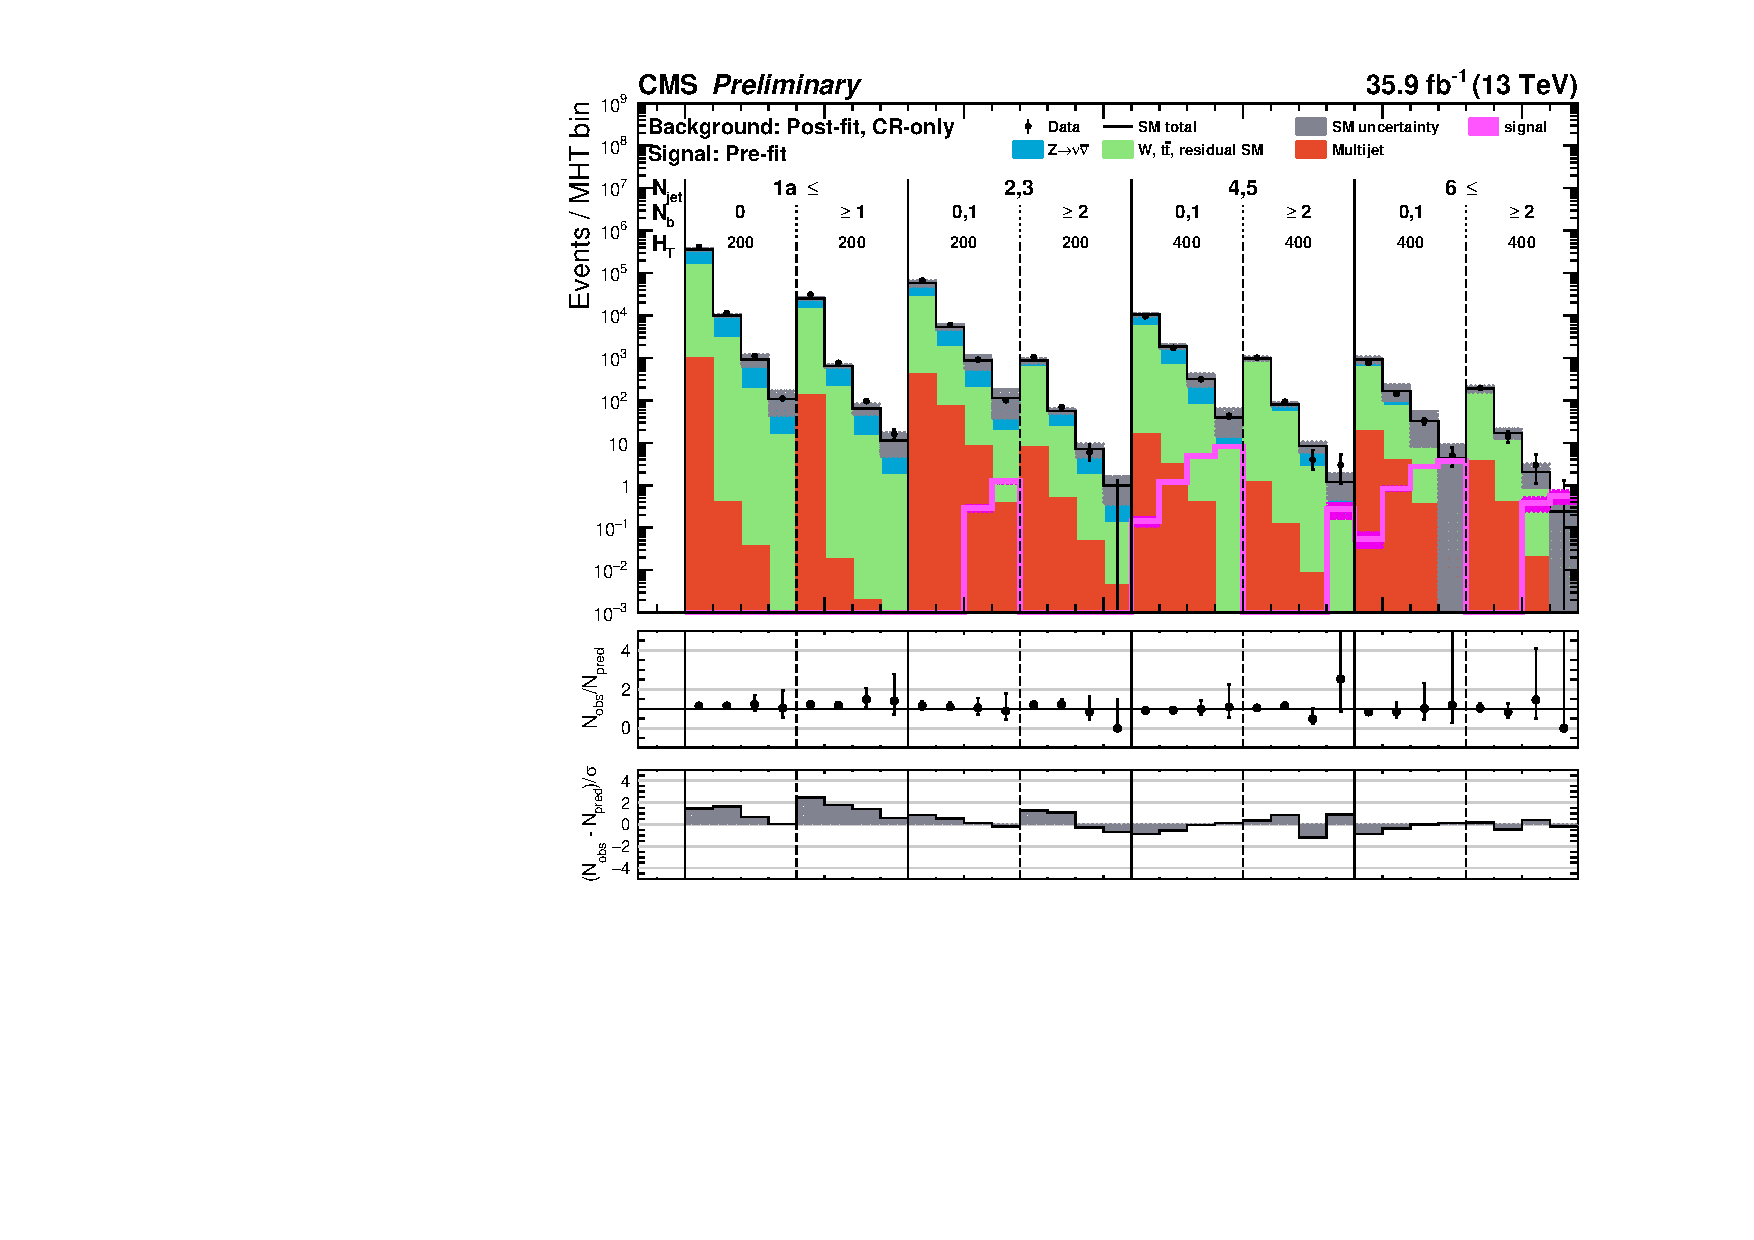
\includegraphics[width=0.49\textwidth]{figures/susyLLResults/app/T1qqqqLL_ctau_0p001_mGluino-1800_mLSP-200/all_full-fit-sig}
        \label{fig:T1qqqqLL_ctau_0p001_uncompressed_MR_simp}
    } ~~
    \subfigure[$c\tau=0.001\unit{mm}$, compressed $(1000,900)$]{
        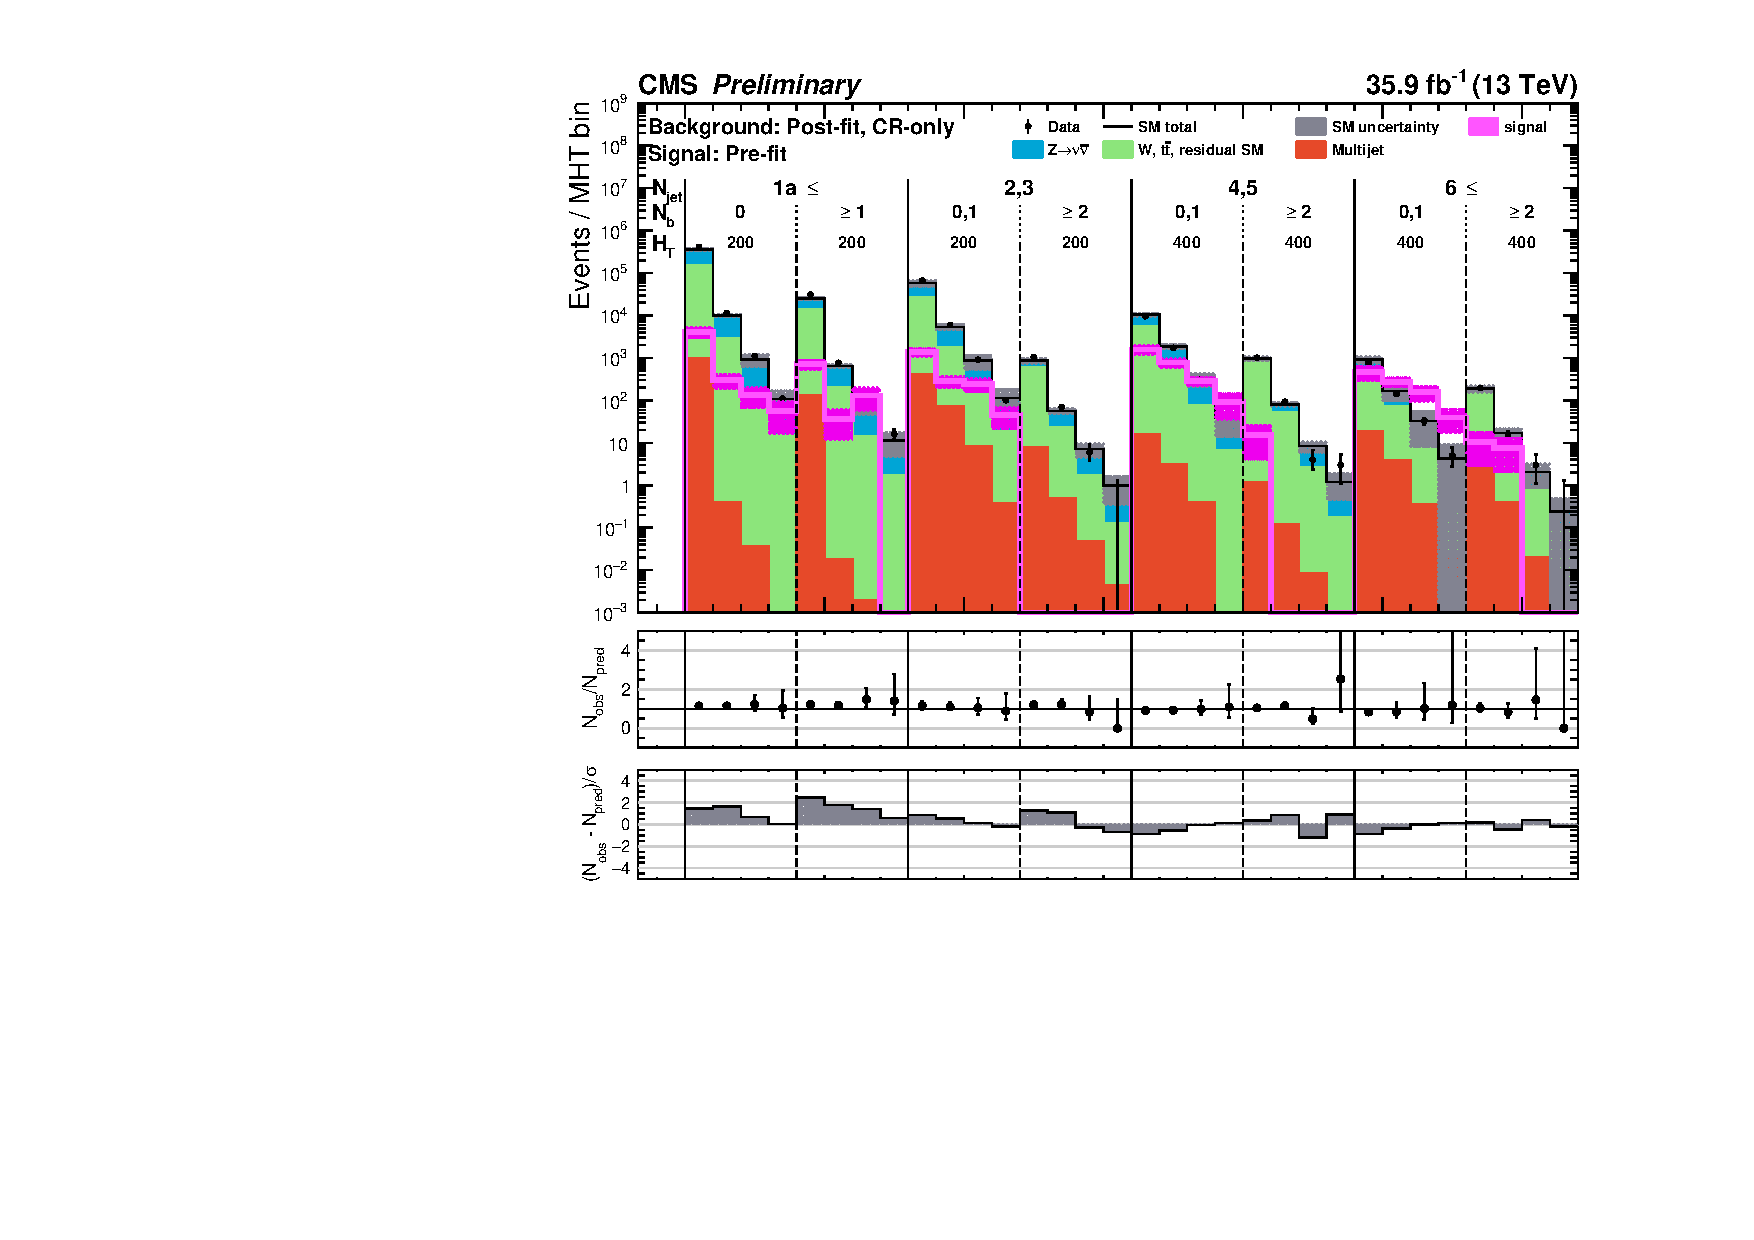
\includegraphics[width=0.49\textwidth]{figures/susyLLResults/app/T1qqqqLL_ctau_0p001_mGluino-1000_mLSP-900/all_full-fit-sig}
        \label{fig:T1qqqqLL_ctau_0p001_compressed_MR_simp}
    } \\
    \subfigure[$c\tau=1\unit{mm}$, uncompressed $(1800,200)$]{
        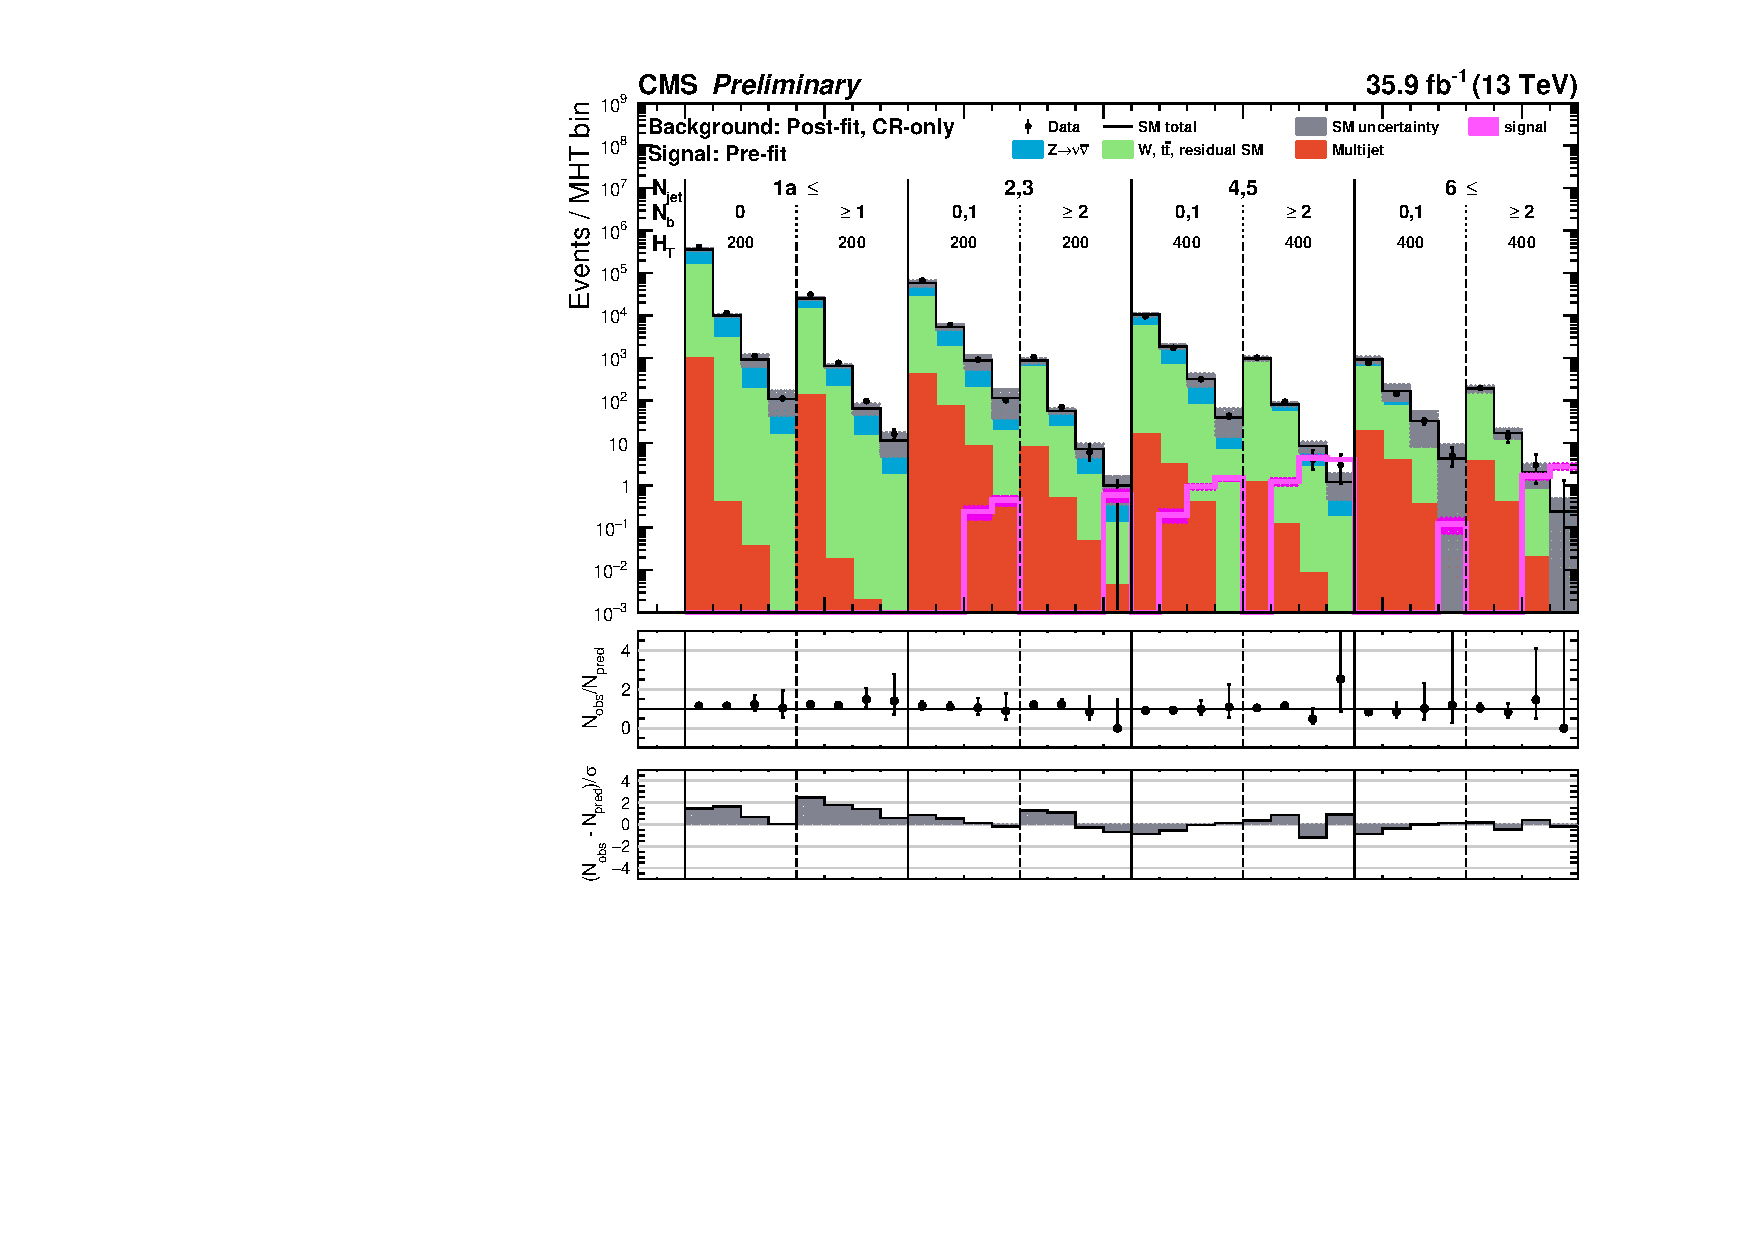
\includegraphics[width=0.49\textwidth]{figures/susyLLResults/app/T1qqqqLL_ctau_1_mGluino-1800_mLSP-200/all_full-fit-sig}
        \label{fig:T1qqqqLL_ctau_1_compressed_MR_simp}
    } ~~
    \subfigure[$c\tau=1\unit{mm}$, compressed $(1000,900)$]{
        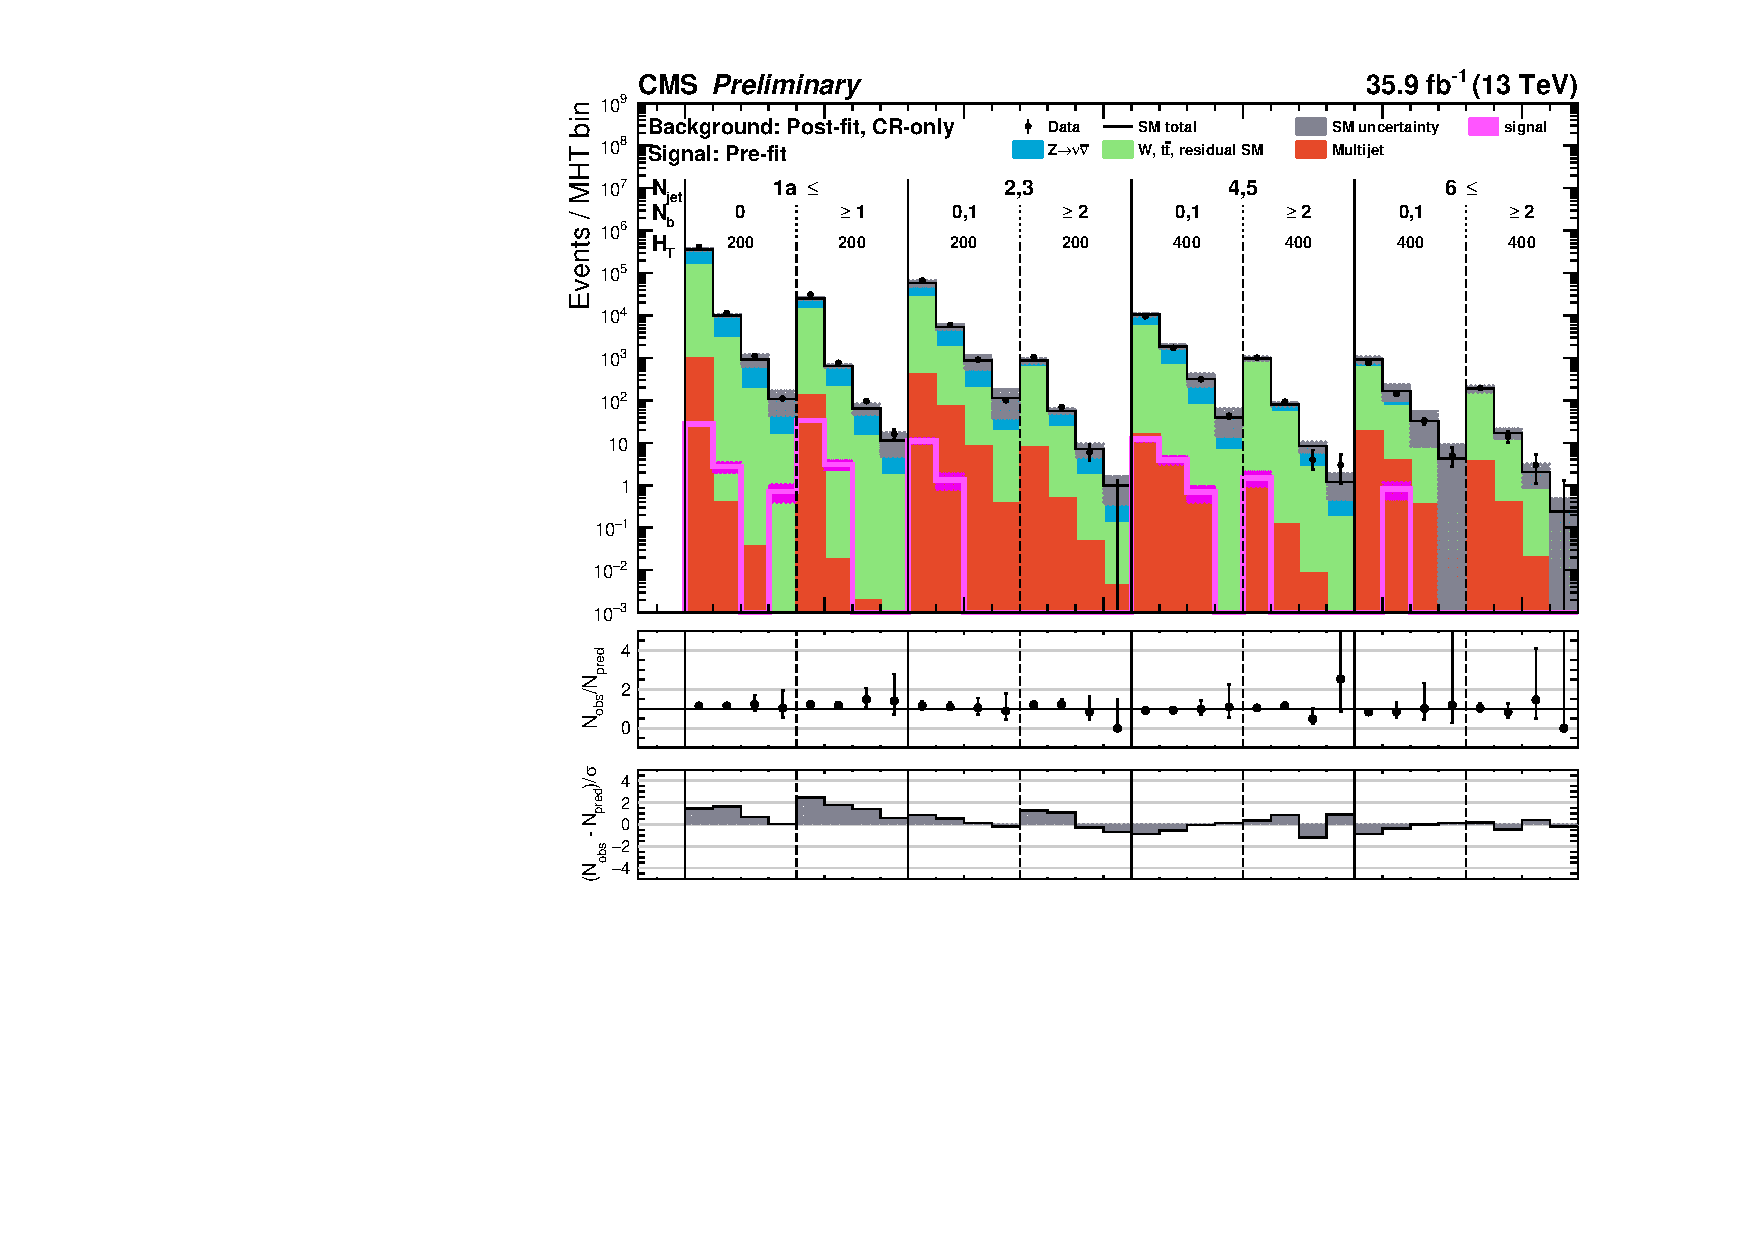
\includegraphics[width=0.49\textwidth]{figures/susyLLResults/app/T1qqqqLL_ctau_1_mGluino-1200_mLSP-1100/all_full-fit-sig}
        \label{fig:T1qqqqLL_ctau_1_uncompressed_MR_simp}
    } \\
    \subfigure[$\ctau=100000\unit{mm}$, uncompressed $(1000,200)$]{
        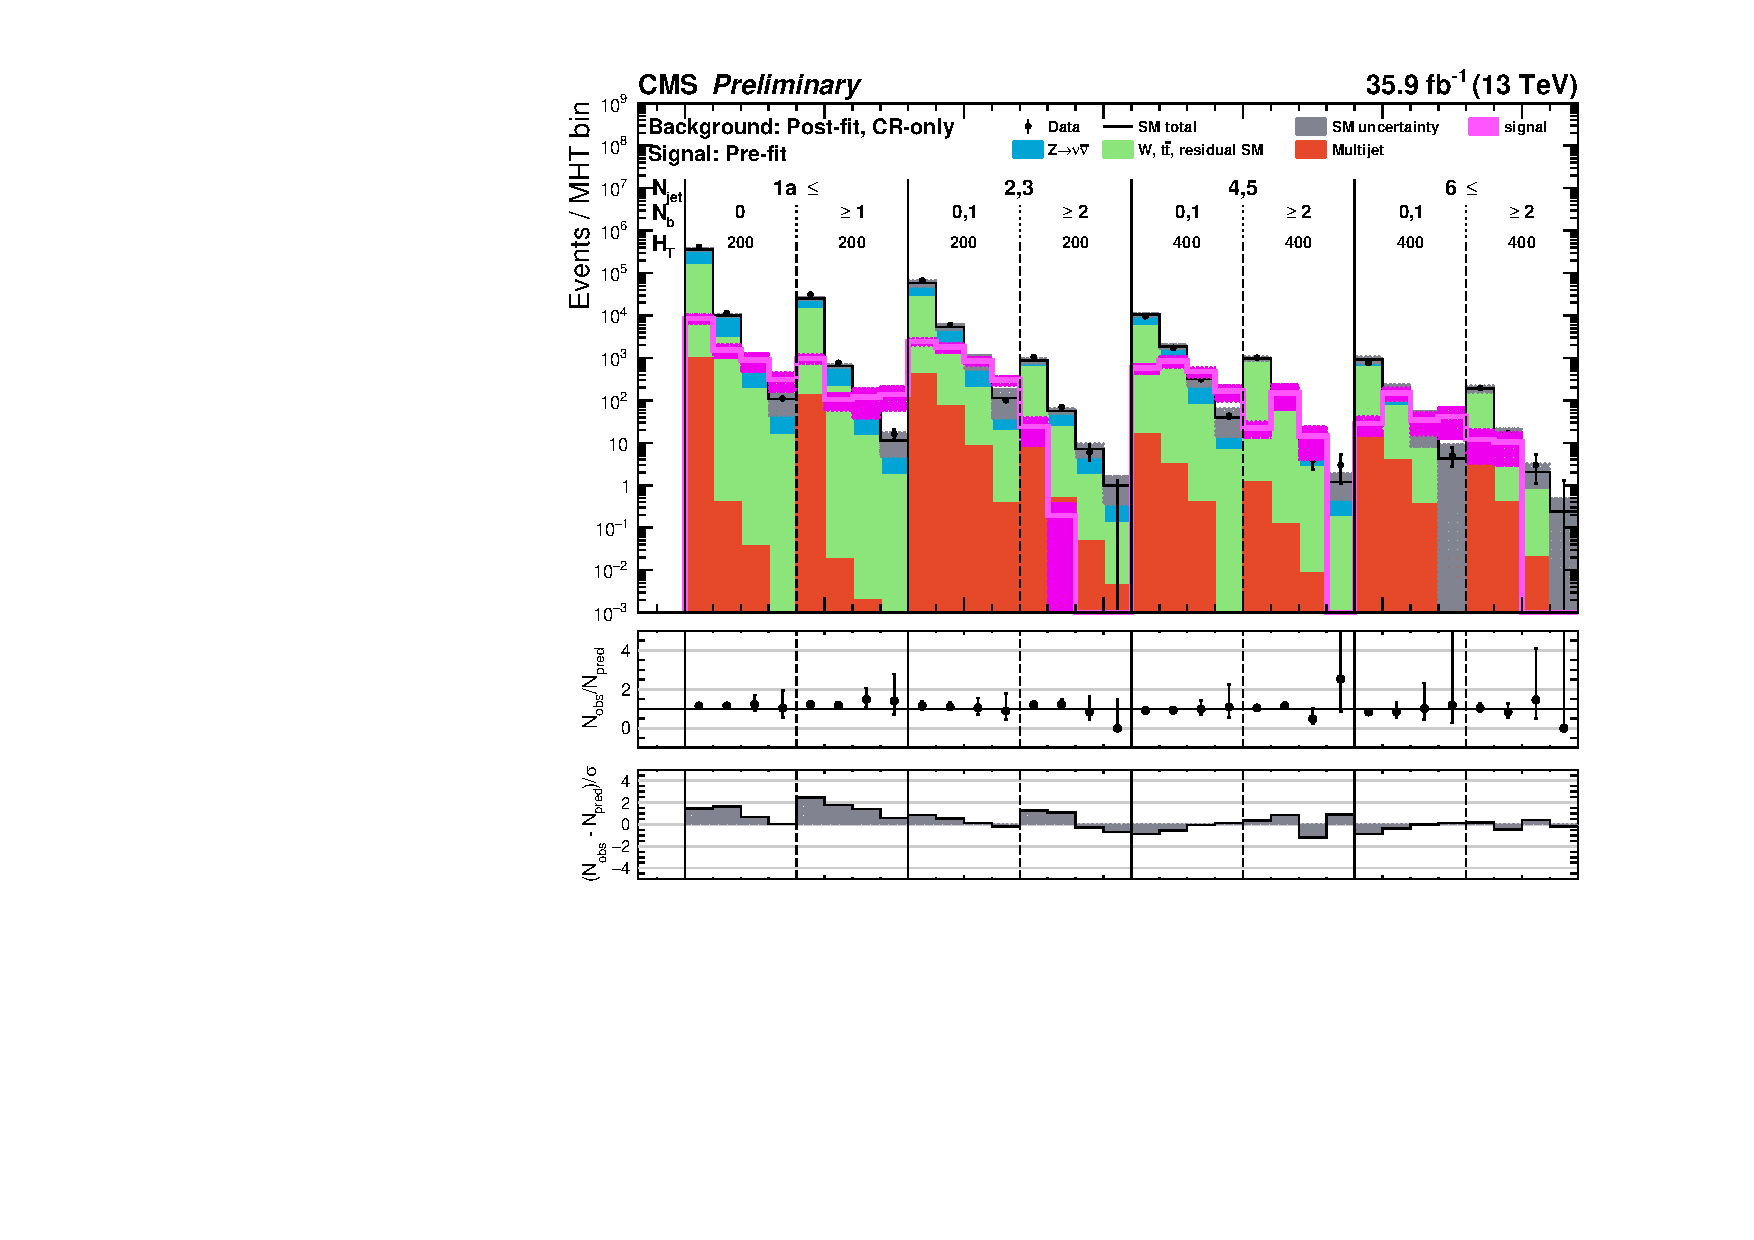
\includegraphics[width=0.49\textwidth]{figures/susyLLResults/app/T1qqqqLL_ctau_100000_mGluino-1000_mLSP-200/all_full-fit-sig}
        \label{fig:T1qqqqLL_ctau_100000_compressed_MR_simp}
    } ~~
    \subfigure[$\ctau=100000\unit{mm}$, compressed $(1000,900)$]{
        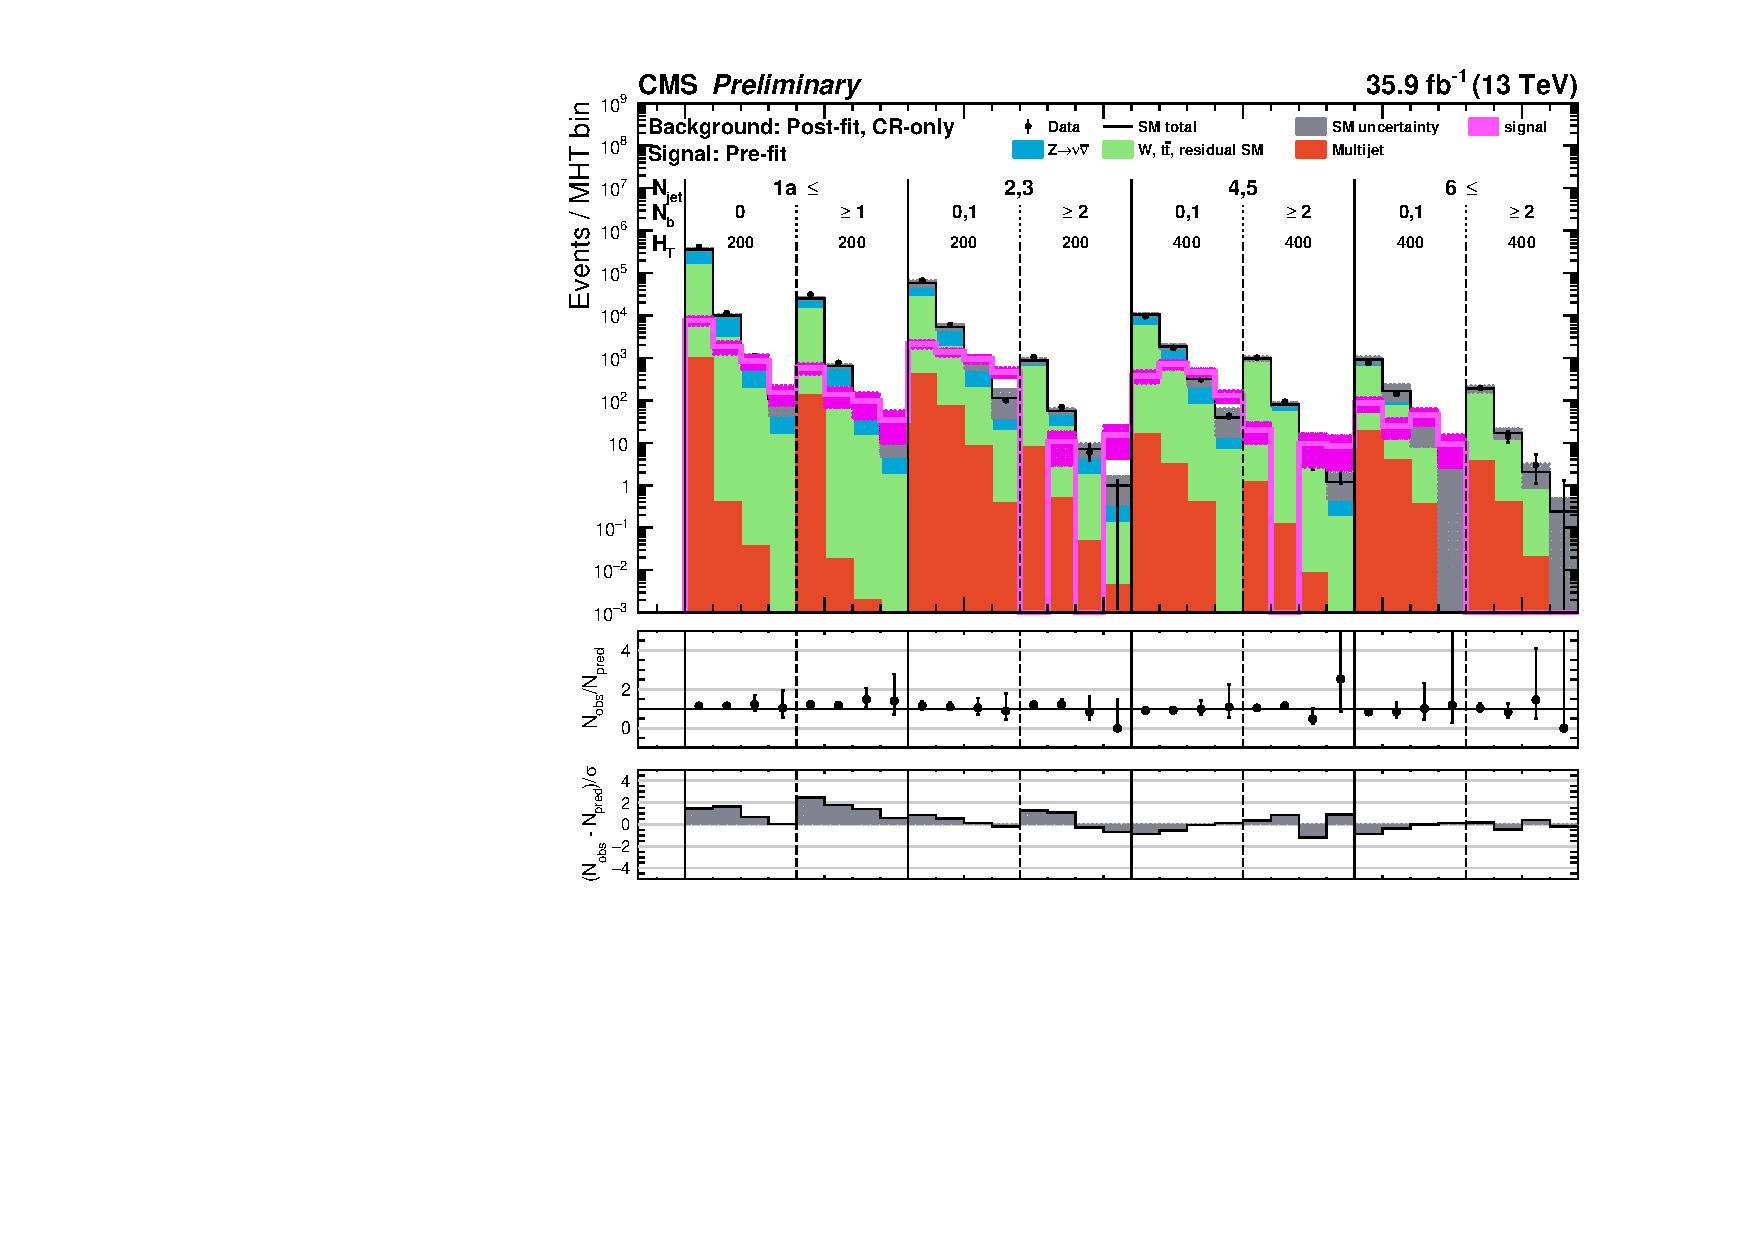
\includegraphics[width=0.49\textwidth]{figures/susyLLResults/app/T1qqqqLL_ctau_100000_mGluino-1000_mLSP-900/all_full-fit-sig}
        \label{fig:T1qqqqLL_ctau_100000_uncompressed_MR_simp}
    } \\
    \caption{ Signal shapes for the \texttt{T1qqqqLL}
      $c\tau=0.001\unit{mm}$ (upper), $c\tau=1\unit{mm}$ (middle), and
      $c\tau=100000\unit{mm}$ (lower) benchmark models with
      uncompressed (left) and compressed (right) mass spectra,
      overlaid on CR-only post-fit background predictions with the
      simplified binning schema.  }
    \label{fig:T1qqqqLL_MR_simp}
\end{figure}

\clearpage
\subsection{Signal acceptance times efficiency}
\label{sec:sig-accept-contam-LLP}

In Tab. \ref{tab:sig-eff-LLP} the signal efficiency for benchmark mass
points and lifetimes (as \ctau) is summarised.
% Signal efficiency figures across ctau vs mass plane?
%The signal efficiency across
%the whole ($m_{\mathrm{Susy}},m_{\mathrm{LSP}}$) for the simplified
%models used in the analysis is shown in
%Figs.~\ref{fig:T1qqqq_eff}-\ref{fig:T2cc_eff}.

\begin{table}[h!]
  \caption{Signal efficiency for T1qqqqLL with different \ctau values.}
  \label{tab:sig-eff-LLP}
  \centering
  \begin{tabular}{lcc}
    \hline \hline
    \ctau (mm) & ($m_{\mathrm{Susy}},m_{\mathrm{LSP}}$) & Efficiency (total) \\ 
    \hline
    \multirow{2}{*}{$0.001$}
    & (1800, 200) & 27.8\% \\
    & (1000, 900) & 6.7\% \\
    \hline
    \multirow{2}{*}{$1$}
    & (1800, 200) & 22.9\% \\
    & (1000, 900) & 5.2\% \\
    \hline
    \multirow{2}{*}{$100000$}
    & (1000, 200) & 11.2\% \\
    & (1000, 900) & 10.4\% \\
    \hline \hline
  \end{tabular}
\end{table}

% Discuss: Variation of Signal Efficiency around B-lifetime ?
% Discuss: Signal contamination of the CRs?  Generally not an issue since no leptons. Sidebands?

Tables~\ref{tab:cut_flow_ctau_0p001}--\ref{tab:cut_flow_ctau_100000}
provide a summary of the cumulative signal acceptance times
efficiency, $\mathcal{A}\,\varepsilon$ [\%], for the \text{T1qqqqLL}
benchmark models, following the application of the event selection
criteria used to define the signal region. 
%The final value in each table represents the efficiency for the
%sensitive topological (\njet, \nb) region defined in
%Table~\ref{tab:benchmark-LLP}.

\clearpage
\begin{table}[!h]
  \caption{Cut flow table for \texttt{T1qqqqLL} models with $c\tau = 0.001\unit{mm}$.} 
  \label{tab:cut_flow_ctau_0p001}
{\scriptsize%resizebox{\textwidth}{!}{
\centering
\begin{tabular}{lcc}
  \hline
  Event selection & \multicolumn{2}{c}{Benchmark model ($m_\mathrm{SUSY},\,m_\mathrm{LSP},\,c\tau$)} \\
  \cline{2-3}
   & T1qqqqLL & T1qqqqLL \\
   & (1800,\,200,\,0.001) & (1000,\,900,\,0.001) \\
  \hline
  Before selection & 100\phantom{.1} & 100\phantom{.1} \\
  Event veto for muons and electrons & \phantom{1}99\phantom{.1} & 100\phantom{.1} \\
  Event veto for single isolated tracks & \phantom{1}92\phantom{.1} & \phantom{1}89\phantom{.1}  \\
  Event veto for photons & \phantom{1}91\phantom{.1} & \phantom{1}88\phantom{.1} \\
   $n_{\mathrm{jet}} \geq 2$ & \phantom{1}91\phantom{.1} & \phantom{1}77\phantom{.1}  \\
   $p_{\mathrm{T}}^{\mathrm{j_1}} > 100\,\mathrm{GeV}$ & \phantom{1}91\phantom{.1} & \phantom{1}50\phantom{.1} \\
   $H_{\mathrm{T}} > 200\,\mathrm{GeV}$ & \phantom{1}91\phantom{.1} & \phantom{1}46\phantom{.1}  \\
  $H_{\mathrm{T}}^{\mathrm{miss}} > 200\,\mathrm{GeV}$ & \phantom{1}85\phantom{.1} & \phantom{1}24\phantom{.1}  \\
  Event veto for forward jets ($|\eta| > 2.4$) & \phantom{1}80\phantom{.1} & \phantom{1}22\phantom{.1}  \\
  $H_{\mathrm{T}}^{\mathrm{miss}} / E_{\mathrm{T}}^{\mathrm{miss}} < 1.25$ & \phantom{1}79\phantom{.1} & \phantom{1}20\phantom{.1}  \\
  $H_{\mathrm{T}}$-dependent $\alpha_{\mathrm{T}}$ requirements ($H_{\mathrm{T}} < 900\,\mathrm{GeV}$) & \phantom{1}79\phantom{.1} & \phantom{1}14\phantom{.1} \\
  $\Delta\phi^{*}_{\mathrm{min}} > 0.5$ & \phantom{1}25\phantom{.1} & \phantom{10}8.7  \\
%  \hline
%  Most sensitive simplified $n_{\mathrm{jet}}$, $n_{\mathrm{b}}$ category & \phantom{10}2.6 & \phantom{10}6.9 \\
  \hline
\end{tabular}
}
\end{table}

\begin{table}[!h]
  \caption{Cut flow table for \texttt{T1qqqqLL} models with $c\tau = 1\unit{mm}$.} 
  \label{tab:cut_flow_ctau_1}
{\scriptsize%resizebox{\textwidth}{!}{\
\centering
\begin{tabular}{lcc}
  \hline
  Event selection & \multicolumn{2}{c}{Benchmark model ($m_\mathrm{SUSY},\,m_\mathrm{LSP},\,c\tau$)} \\
  \cline{2-3}
   & T1qqqqLL & T1qqqqLL \\
    & (1800,\,200,\,1) & (1000,\,900,\,1) \\
  \hline
  Before selection  & 100\phantom{.1} & 100\phantom{.1} \\
  Event veto for muons and electrons & \phantom{1}99\phantom{.1} & \phantom{1}99\phantom{.1} \\
  Event veto for single isolated tracks & \phantom{1}84\phantom{.1} & \phantom{1}90\phantom{.1} \\
  Event veto for photons & \phantom{1}83\phantom{.1} & \phantom{1}89\phantom{.1} \\
   $n_{\mathrm{jet}} \geq 2$  & \phantom{1}83\phantom{.1} & \phantom{1}74\phantom{.1} \\
   $p_{\mathrm{T}}^{\mathrm{j_1}} > 100\,\mathrm{GeV}$ & \phantom{1}83\phantom{.1} & \phantom{1}48\phantom{.1} \\
   $H_{\mathrm{T}} > 200\,\mathrm{GeV}$  & \phantom{1}83\phantom{.1} & \phantom{1}44\phantom{.1} \\
  $H_{\mathrm{T}}^{\mathrm{miss}} > 200\,\mathrm{GeV}$  & \phantom{1}78\phantom{.1} & \phantom{1}23\phantom{.1} \\
  Event veto for forward jets ($|\eta| > 2.4$) & \phantom{1}74\phantom{.1} & \phantom{1}21\phantom{.1} \\
  $H_{\mathrm{T}}^{\mathrm{miss}} / E_{\mathrm{T}}^{\mathrm{miss}} < 1.25$ & \phantom{1}70\phantom{.1} & \phantom{1}20\phantom{.1} \\
  $H_{\mathrm{T}}$-dependent $\alpha_{\mathrm{T}}$ requirements ($H_{\mathrm{T}} < 900\,\mathrm{GeV}$)  & \phantom{1}70\phantom{.1} & \phantom{1}13\phantom{.1} \\
  $\Delta\phi^{*}_{\mathrm{min}} > 0.5$  & \phantom{1}24\phantom{.1} & \phantom{10}8.1 \\
%  \hline
%  Most sensitive simplified $n_{\mathrm{jet}}$, $n_{\mathrm{b}}$ category & \phantom{10}1.8 & \phantom{10}5.4 \\
  \hline
\end{tabular}
}
\end{table}

\begin{table}[!h]
  \caption{Cut flow table for \texttt{T1qqqqLL} models with $c\tau = 100000\unit{mm}$.} 
  \label{tab:cut_flow_ctau_100000}
{\scriptsize%\resizebox{\textwidth}{!}{
\centering
\begin{tabular}{lcc}
  \hline
  Event selection & \multicolumn{2}{c}{Benchmark model ($m_\mathrm{SUSY},\,m_\mathrm{LSP},\,c\tau$)} \\
  \cline{2-3}
   & T1qqqqLL & T1qqqqLL \\
    & (1000,\,200,\,10$^5$) & (1000,\,900,\,10$^5$) \\
  \hline
  Before selection  & 100\phantom{.1} & 100\phantom{.1} \\
  Event veto for muons and electrons & 100\phantom{.1} & 100\phantom{.1} \\
  Event veto for single isolated tracks & \phantom{1}97\phantom{.1} & \phantom{1}97\phantom{.1} \\
  Event veto for photons & \phantom{1}97\phantom{.1} & \phantom{1}97\phantom{.1} \\
   $n_{\mathrm{jet}} \geq 2$  & \phantom{1}41\phantom{.1} & \phantom{1}39\phantom{.1} \\
   $p_{\mathrm{T}}^{\mathrm{j_1}} > 100\,\mathrm{GeV}$ & \phantom{1}34\phantom{.1} & \phantom{1}30\phantom{.1} \\
   $H_{\mathrm{T}} > 200\,\mathrm{GeV}$  & \phantom{1}31\phantom{.1} & \phantom{1}27\phantom{.1} \\
  $H_{\mathrm{T}}^{\mathrm{miss}} > 200\,\mathrm{GeV}$  & \phantom{1}23\phantom{.1} & \phantom{1}19\phantom{.1} \\
  Event veto for forward jets ($|\eta| > 2.4$) & \phantom{1}21\phantom{.1} & \phantom{1}17\phantom{.1} \\
  $H_{\mathrm{T}}^{\mathrm{miss}} / E_{\mathrm{T}}^{\mathrm{miss}} < 1.25$ & \phantom{1}20\phantom{.1} & \phantom{1}17\phantom{.1} \\
  $H_{\mathrm{T}}$-dependent $\alpha_{\mathrm{T}}$ requirements ($H_{\mathrm{T}} < 900\,\mathrm{GeV}$)  &  \phantom{1}14 \phantom{.1} & \phantom{1}12\phantom{.1} \\
  $\Delta\phi^{*}_{\mathrm{min}} > 0.5$  &  \phantom{1}11\phantom{.1} & \phantom{1}10\phantom{.1} \\
%  \hline
%  Most sensitive simplified $n_{\mathrm{jet}}$, $n_{\mathrm{b}}$ category & \phantom{10}0.4 & \phantom{10}8.1 \\
  \hline
\end{tabular}
}
\end{table}

\clearpage
\subsection{Systematic uncertainties on signal efficiency times acceptance}
\label{sec:sig-syst-LLP}

The following sources of systematic uncertainty are propagated to the
signal acceptance and shape, according to the recommendations agreed
on within the collaboration. Relative effect on the yields are
presented in Tab.~\ref{tab:sig-systematics-LLP} for some benchmark
models.

\begin{itemize}
    \item Luminosity: 2.6\%, taken as correlated across all bins.
    \item Trigger: conservatively, the size of the inefficiency is taken as
        systematic variation where not in the plateau (see Sec.~\ref{sec:triggers}).
    \item MC statistics:  uncorrelated bin-by-bin uncertainty, affecting the
        shape of the signal.
    \item Pileup reweighting: 5.0\% uncertainty on the minimum bias cross section
        (see Sec.~\ref{sec:pileup-reweighting}).
    \item b-tag efficiency: uncertainty on the FullSim b-tag scale
        factor is propagated and taken as correlated across the bins.
    \item mis-tag efficiency: uncertainty on the FullSim mis-tag scale
        factor is propagated and taken as correlated across the bins.
    \item Lepton efficiency: uncertainty on the lepton scale factors is
        propagated and taken as correlated across the bins.
    \item Jet energy scale: uncertainty on the jet energy corrections is
        propagated and taken as correlated across the bins.
    \item Initial State Radiation (ISR): Reweighting of the $N_{\text{isr}}$
        distribution. The systematic is taken as half the corrections.
\end{itemize}

\begin{table}[h!]
        % TODO CHANGE THIS TABLE
    \scriptsize
    \caption{
        Representative range taken from the $16\%$ and $84\%$ percentiles of the
        uncertainty across the analysis bins for each source of signal
        systematic. Two benchmark point are chosen for each model, corresponding
        to ``compressed'' and ``uncompressed'' scenarios, i.e. with small and
        large mass splitting between the mother particle and the LSP. 
    }
    \label{tab:sig-systematics-LLP}
    \centering
    \begin{tabular}{ cccccccccc }
      \hline \hline
      $c\tau$ [mm] & ($m_{\mathrm{Susy}},m_{\mathrm{LSP}}$) 
      & Luminosity & ISR   & JECs   & PU     & b-tag & mis-tag & Trigger & MC stat.        \\ 
      \hline
      \multirow{2}{*}{0.001}
      & (1800,200) & 2.6\% & 3-5\%  & 3-6\%  & 1-3\% & 0-0\%   & 2-9\%   & 3-4\% & 8-16\%  \\
      & (1000,900) & 2.6\% & 1-12\% & 3-18\% & 1-3\% & 0-0\%   & 0-1\%   & 0-2\% & 13-24\% \\
      \hline
      \multirow{2}{*}{1}
      & (1800,200) & 2.6\% & 2-4\%  & 3-9\%  & 2-4\% & 3-16\%  & 3-14\%  & 2-4\% & 17-22\% \\
      & (1000,900) & 2.6\% & 3-9\%  & 5-18\% & 1-4\% & 4-8\%   & 8-13\%  & 0-2\% & 20-29\% \\        
      \hline
      \multirow{2}{*}{100000}
      & (1000,200) & 2.6\% & 2-17\% & 4-13\% & 1-5\% & 0-1\%   & 1-1\%   & 0-4\% & 16-30\% \\
      & (1000,900) & 2.6\% & 3-14\% & 4-11\% & 1-5\% & 0-0\%   & 1-1\%   & 0-1\% & 14-25\% \\
      \hline

        \hline \hline
    \end{tabular}
\end{table}

\clearpage
\subsection{Sensitive categories and limits}
\label{sec:LLP_results}

The 95\% CL upper limit on the ratio of the cross section to the
theoretical cross section is repeated with a similar likelihood model
used to obtain the standard limits in Sec.~\ref{sec:susy_results};
however, the combination of analysis bins is varied to understand
which bins drive the sensitivity of the benchmark signal models. The
limits are recalculated with sub-regions of the signal region at
different granularities. The finest granularity considers each \mht
bin within a sub-region defined in terms of (\njet, \nb, \scalht). The
next-finest granularity considered all (\scalht, \mht) bins within
each sub-region defined in terms of (\njet, \nb). Next, sub-regions
defined in terms of only \njet are consdiered, and finally the full
signal region is considered. Figure~\ref{fig:T1qqqqLL_limitsPerBin}
summarises this information, which allows to understand which bins
drive the sensitivity to a particular benchmark model. This procedure
is intended to be illustrative only, as it involves breaking the
assumptions/correlations between the analysis bins.

\begin{figure}[!h]
  \centering
  \subfigure[$c\tau = 0.001\unit{mm}$, uncompressed $(1800,200)$]{
    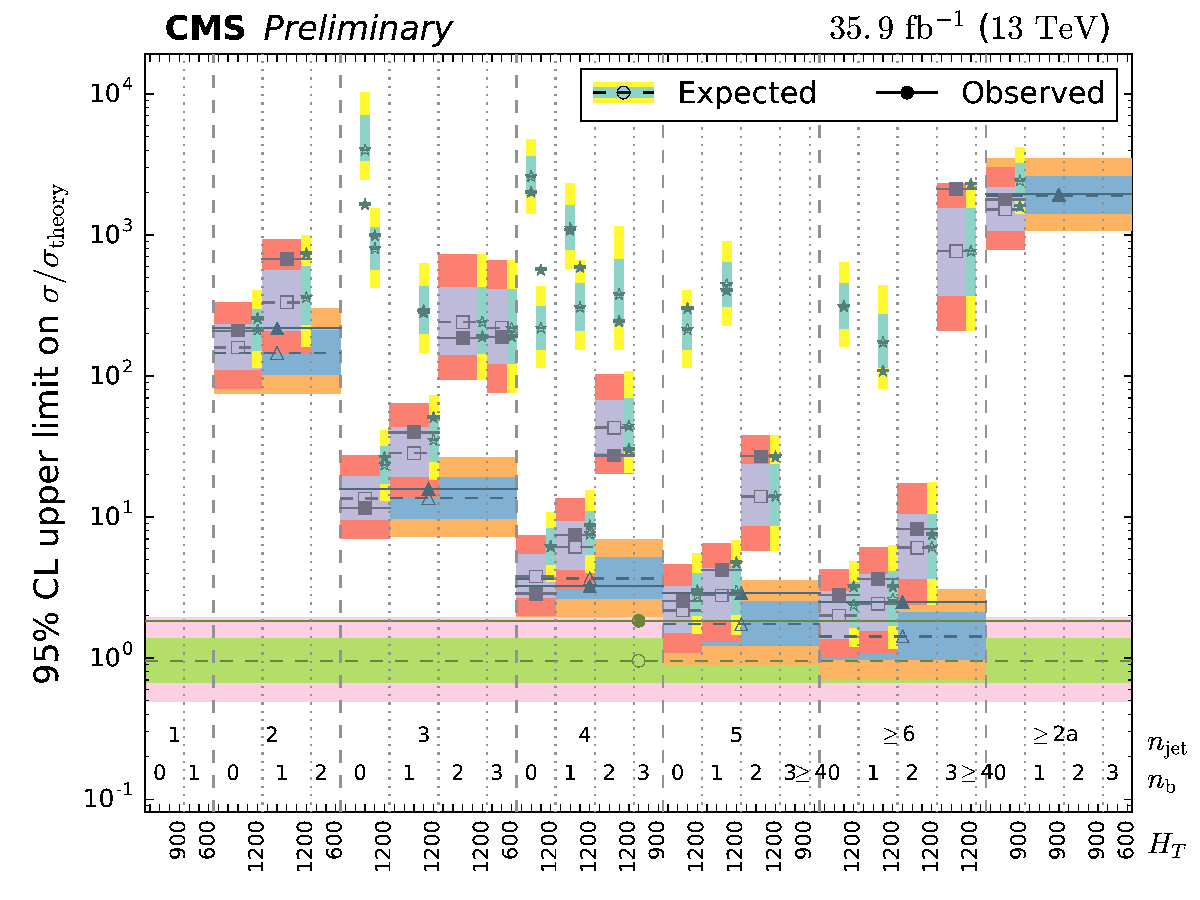
\includegraphics[width=0.49\textwidth]{figures/susyLLResults/app/T1qqqqLL_ctau_0p001_mGluino-1800_mLSP-200/limits_per_bin}
    \label{fig:T1qqqqLL_ctau_0p001_uncompressed_limitsPerBin}
  } ~~
  \subfigure[$c\tau = 0.001\unit{mm}$, compressed $(1000,900)$]{
    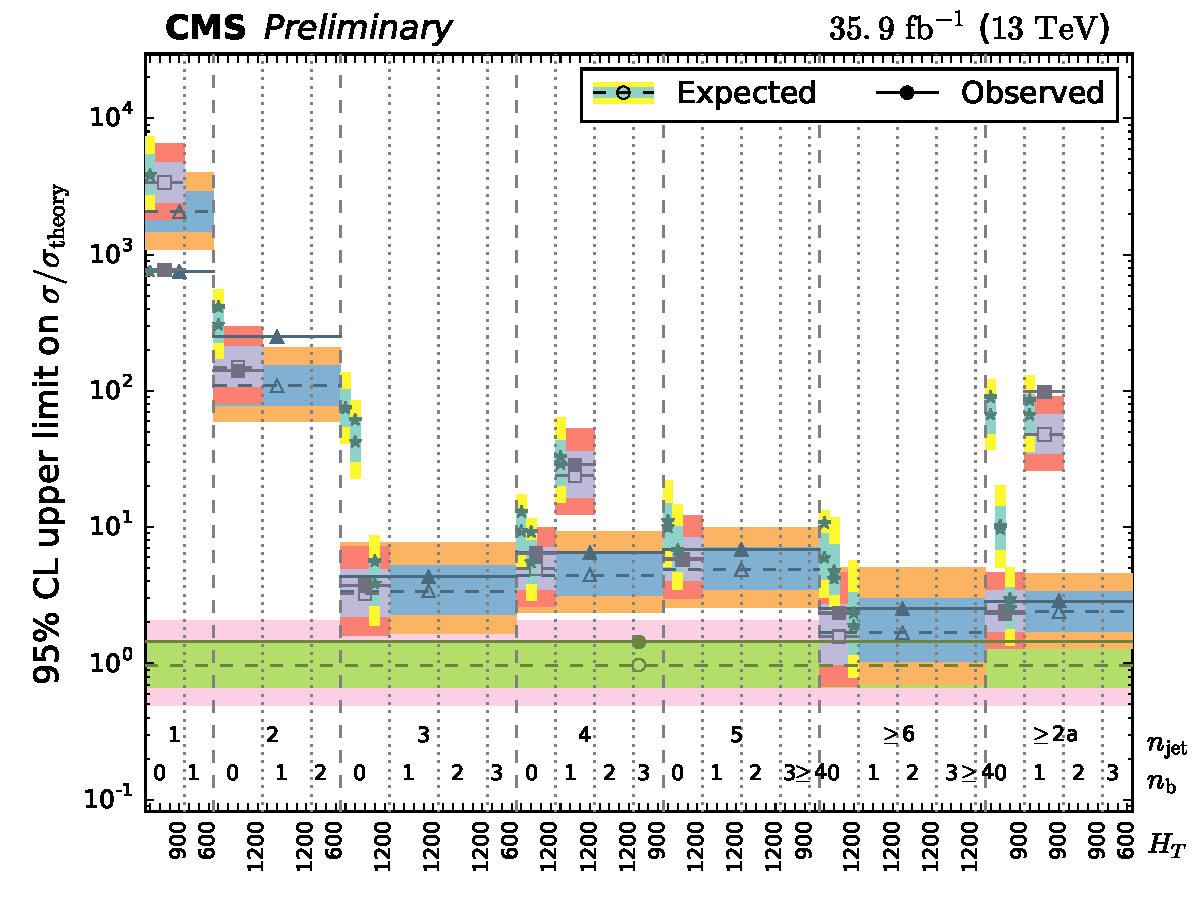
\includegraphics[width=0.49\textwidth]{figures/susyLLResults/app/T1qqqqLL_ctau_0p001_mGluino-1000_mLSP-900/limits_per_bin}
    \label{fig:T1qqqqLL_ctau_0p001_compressed_limitsPerBin}
  } \\
  \subfigure[$c\tau = 1\unit{mm}$, uncompressed $(1800,200)$]{
    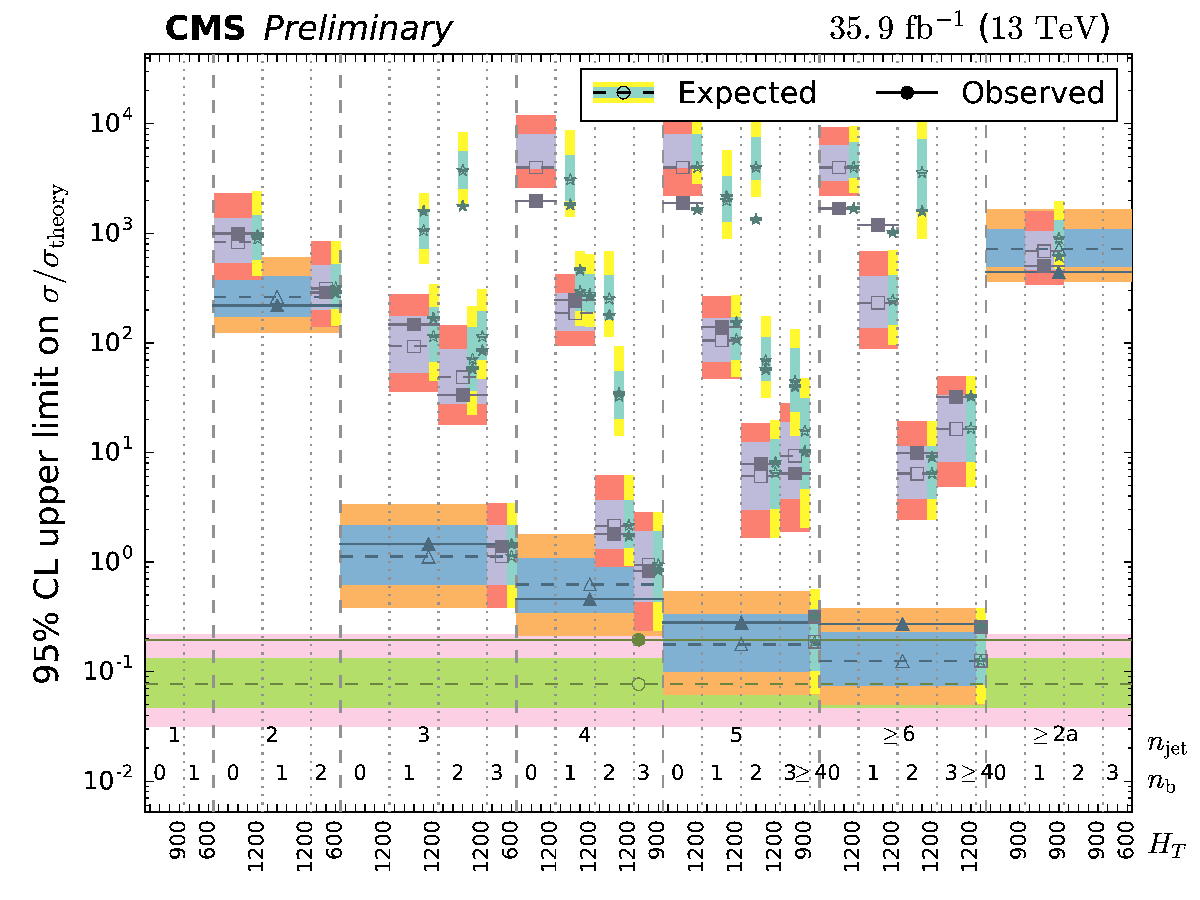
\includegraphics[width=0.49\textwidth]{figures/susyLLResults/app/T1qqqqLL_ctau_1_mGluino-1800_mLSP-200/limits_per_bin}
    \label{fig:T1qqqqLL_ctau_1_uncompressed_limitsPerBin}
  } ~~
  \subfigure[$c\tau = 1\unit{mm}$, compressed $(1000,900)$]{
    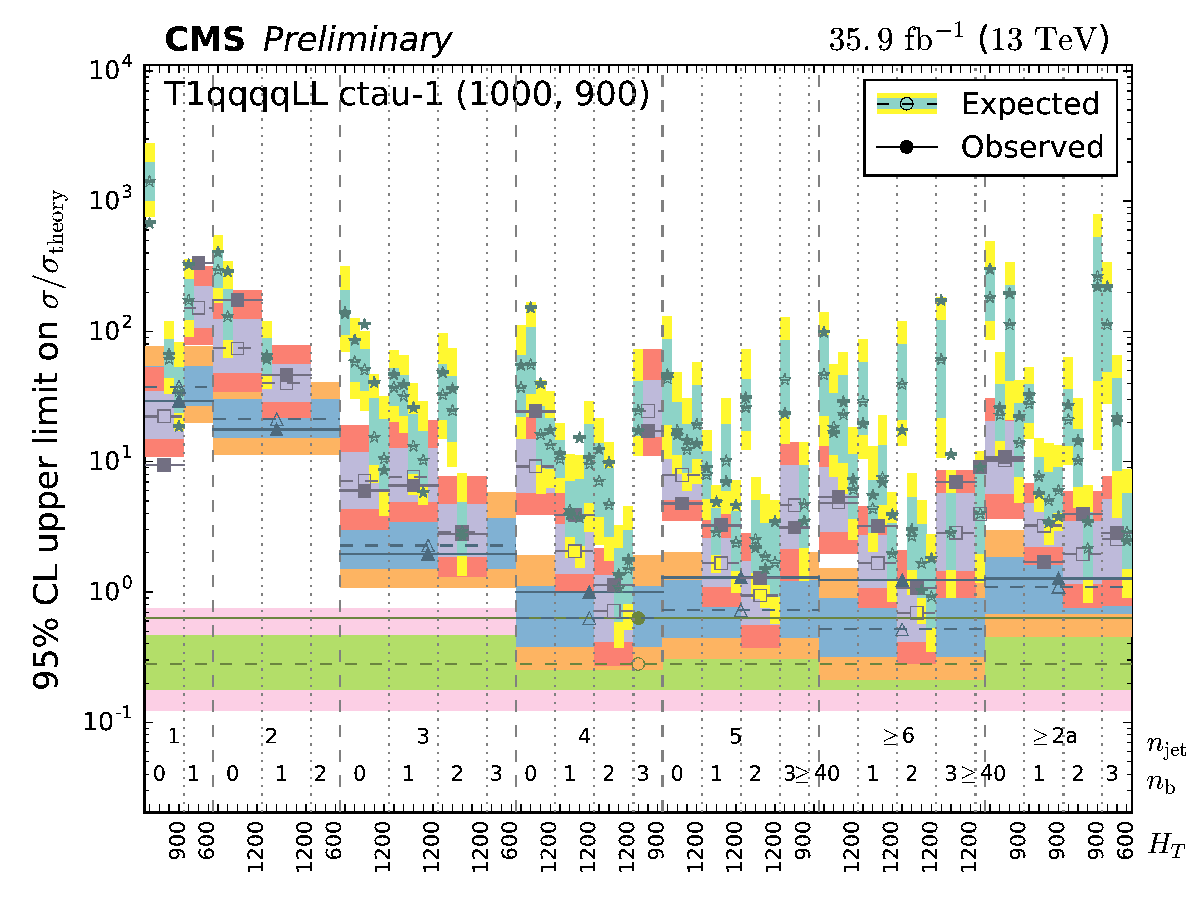
\includegraphics[width=0.49\textwidth]{figures/susyLLResults/app/T1qqqqLL_ctau_1_mGluino-1000_mLSP-900/limits_per_bin}
    \label{fig:T1qqqqLL_ctau_1_compressed_limitsPerBin}
  } \\
  \subfigure[$c\tau = 100000\unit{mm}$, uncompressed $(1000,200)$]{
    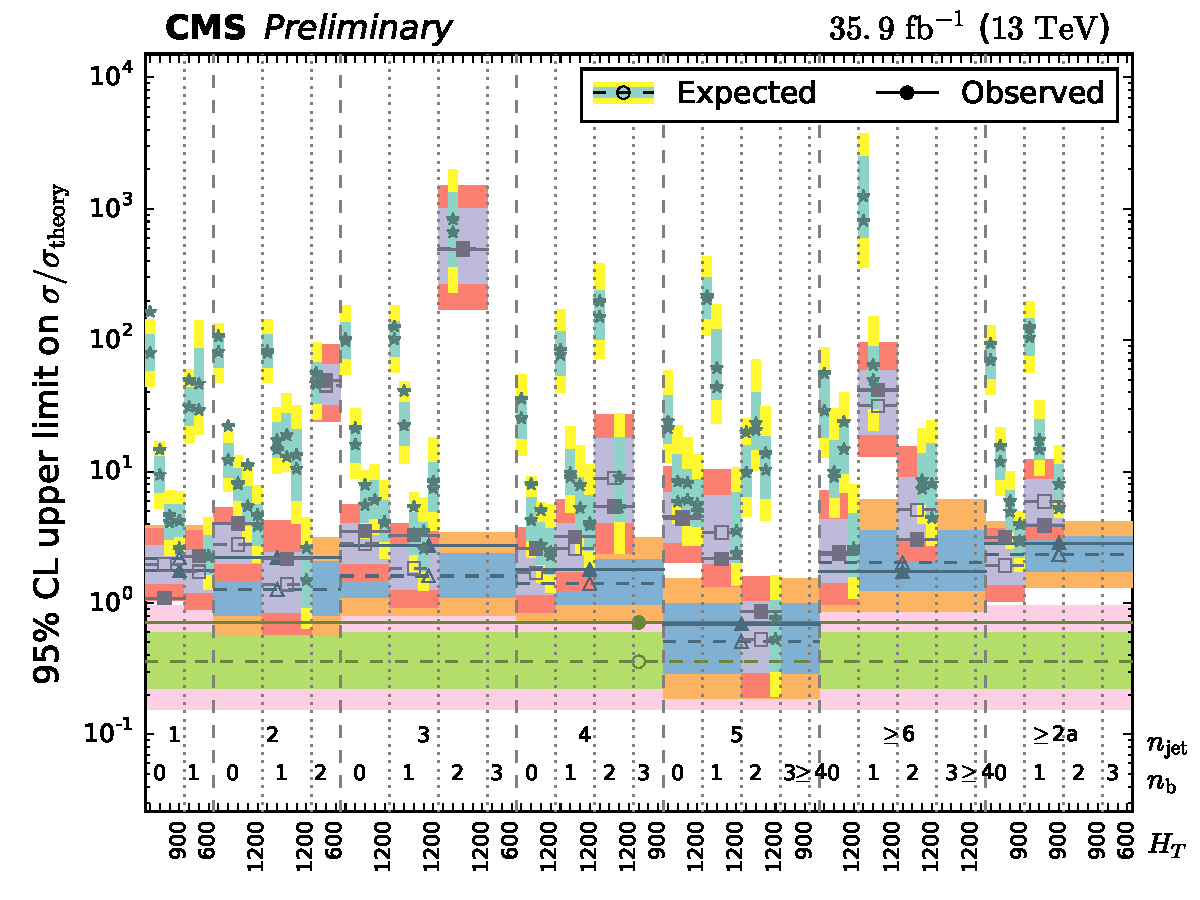
\includegraphics[width=0.49\textwidth]{figures/susyLLResults/app/T1qqqqLL_ctau_100000_mGluino-1000_mLSP-200/limits_per_bin}
    \label{fig:T1qqqqLL_ctau_100000_uncompressed_limitsPerBin}
  } ~~
  \subfigure[$c\tau = 100000\unit{mm}$, compressed $(1000,900)$]{
    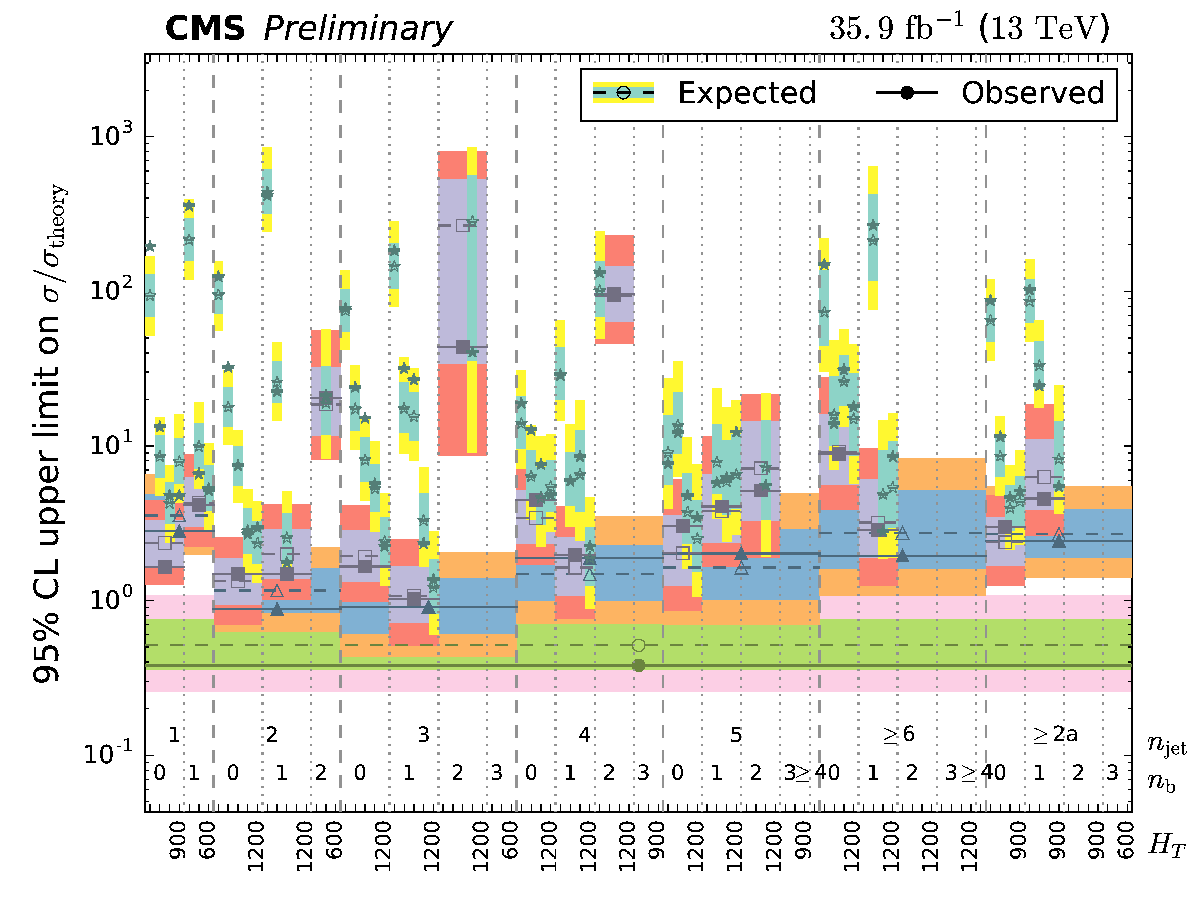
\includegraphics[width=0.49\textwidth]{figures/susyLLResults/app/T1qqqqLL_ctau_100000_mGluino-1000_mLSP-900/limits_per_bin}
    \label{fig:T1qqqqLL_ctau_100000_compressed_limitsPerBin}
  } \\
  \caption{ 95\% CL upper limits on $\sigma/\sigma_{\mathrm{theory}}$
    for the \texttt{T1qqqqLL} benchmark models with
    $c\tau=0.001\unit{mm}$ (upper), $c\tau=1\unit{mm}$ (middle),
    $c\tau=100000\unit{mm}$ (lower) and uncompressed (left) and
    compressed (right) mass spectra. Limits are shown for four
    different granularities of sub-regions: individual (\njet, \nb,
    \scalht) bins, (\njet, \nb) regions, \njet regions; and finally
    the full signal region, all overlaid in ascending order. The
    expected limit, along with the $\pm 1\sigma$ and $\pm 2\sigma$
    bands, and the observed limit are displayed for each bin
    combination. Individual (\njet, \nb, \scalht) bins for which no
    limits is shown are either not included in the search or provide
    negligible sensitivity to the model in question.}
  \label{fig:T1qqqqLL_limitsPerBin}
\end{figure}

Table~\ref{tab:susyLL_aggr_limits} summarises the expected and
observed limits determined for each benchmark model using the nominal
and simplified binning schemas.

\begin{table*}[!h]
  \topcaption{Expected ($\mu_{\text{exp}}$) and observed 
    ($\mu_{\text{obs}}$) upper limits on the production cross section, 
    expressed in terms of the signal strength parameter, obtained using
    both the nominal and simplified binning schemas. 
  }
  \label{tab:susyLL_aggr_limits}
  \centering
  \begin{tabular}{ llccccc }
    \hline
    \multicolumn{2}{c}{Benchmark models} & \multicolumn{2}{c}{Nominal}
                                         & 
                                         & \multicolumn{2}{c}{Simplified}             \\ [0.3ex]
    \cline{3-4}
    \cline{6-7}
   %\multicolumn{2}{c}{$(m_{\text{SUSY}}, m_{\mathrm{LSP}})$ [\GeVns{}]} 
    \ctau [mm] 
                                         & $(m_{\text{SUSY}}, m_{\mathrm{LSP}})$ [\GeVns{}]
                                         & $\mu_{\text{exp}}$
                                         & $\mu_{\text{obs}}$
                                         & 
                                         & $\mu_{\text{exp}}$
                                         & $\mu_{\text{obs}}$                         \\ [0.3ex]
    \hline
    \multirow{2}{*}{0.001}               & (1800, 200) & 0.81 & 1.58 &  & 1.22 & 1.53 \\
                                         & (1000, 900) & 0.95 & 1.21 &  & 2.23 & 2.28 \\ [0.5ex]
    \multirow{2}{*}{1}                   & (1800, 200) & 0.36 & 0.66 &  & 0.47 & 0.44 \\
                                         & (1000, 900) & 1.98 & 2.00 &  & 3.22 & 4.61 \\ [0.5ex]
    \multirow{2}{*}{100000}              & (1000, 200) & 0.95 & 1.33 &  & 1.88 & 2.32 \\
                                         & (1000, 900) & 0.95 & 0.73 &  & 1.90 & 1.47 \\ 
    \hline
  \end{tabular}
\end{table*}

\subsection{Limits in the mass planes}

In Figs.~\ref{fig:T1qqqqLL:ctau-0p001}-\ref{fig:T1qqqqLL:ctau-100000}
the top sub-figure shows the 95\% C.L. upper limits on the cross
section are shown in the $(m_{\mathrm{Susy}},m_{\mathrm{LSP}})$ plane
for the models considered in this interpretation. These results
correspond to 35.9~\ifb of integrated luminosity. The exclusion
contour is also shown together with $\pm1\sigma$ (and $\pm2\sigma$ for
the expected exclusion) uncertainty.  The band around the expected
exclusion reflects the experimental uncertainty, while the band around
the observed exclusion correspond to the theoretical uncertainty on
the signal cross section. The left sub-figure shows the signal
acceptance for each mass point in the SMS scan. In the right
sub-figure, each mass point is labelled with a group of (\njet, \nb)
topologies in descending order of sensitivity. 

\begin{figure}[h!]
    \begin{center}
        \subfigure[T1qqqqLL ($\ctau = 0.001\unit{mm}$): Upper limit on the cross section in the mass plane]{
            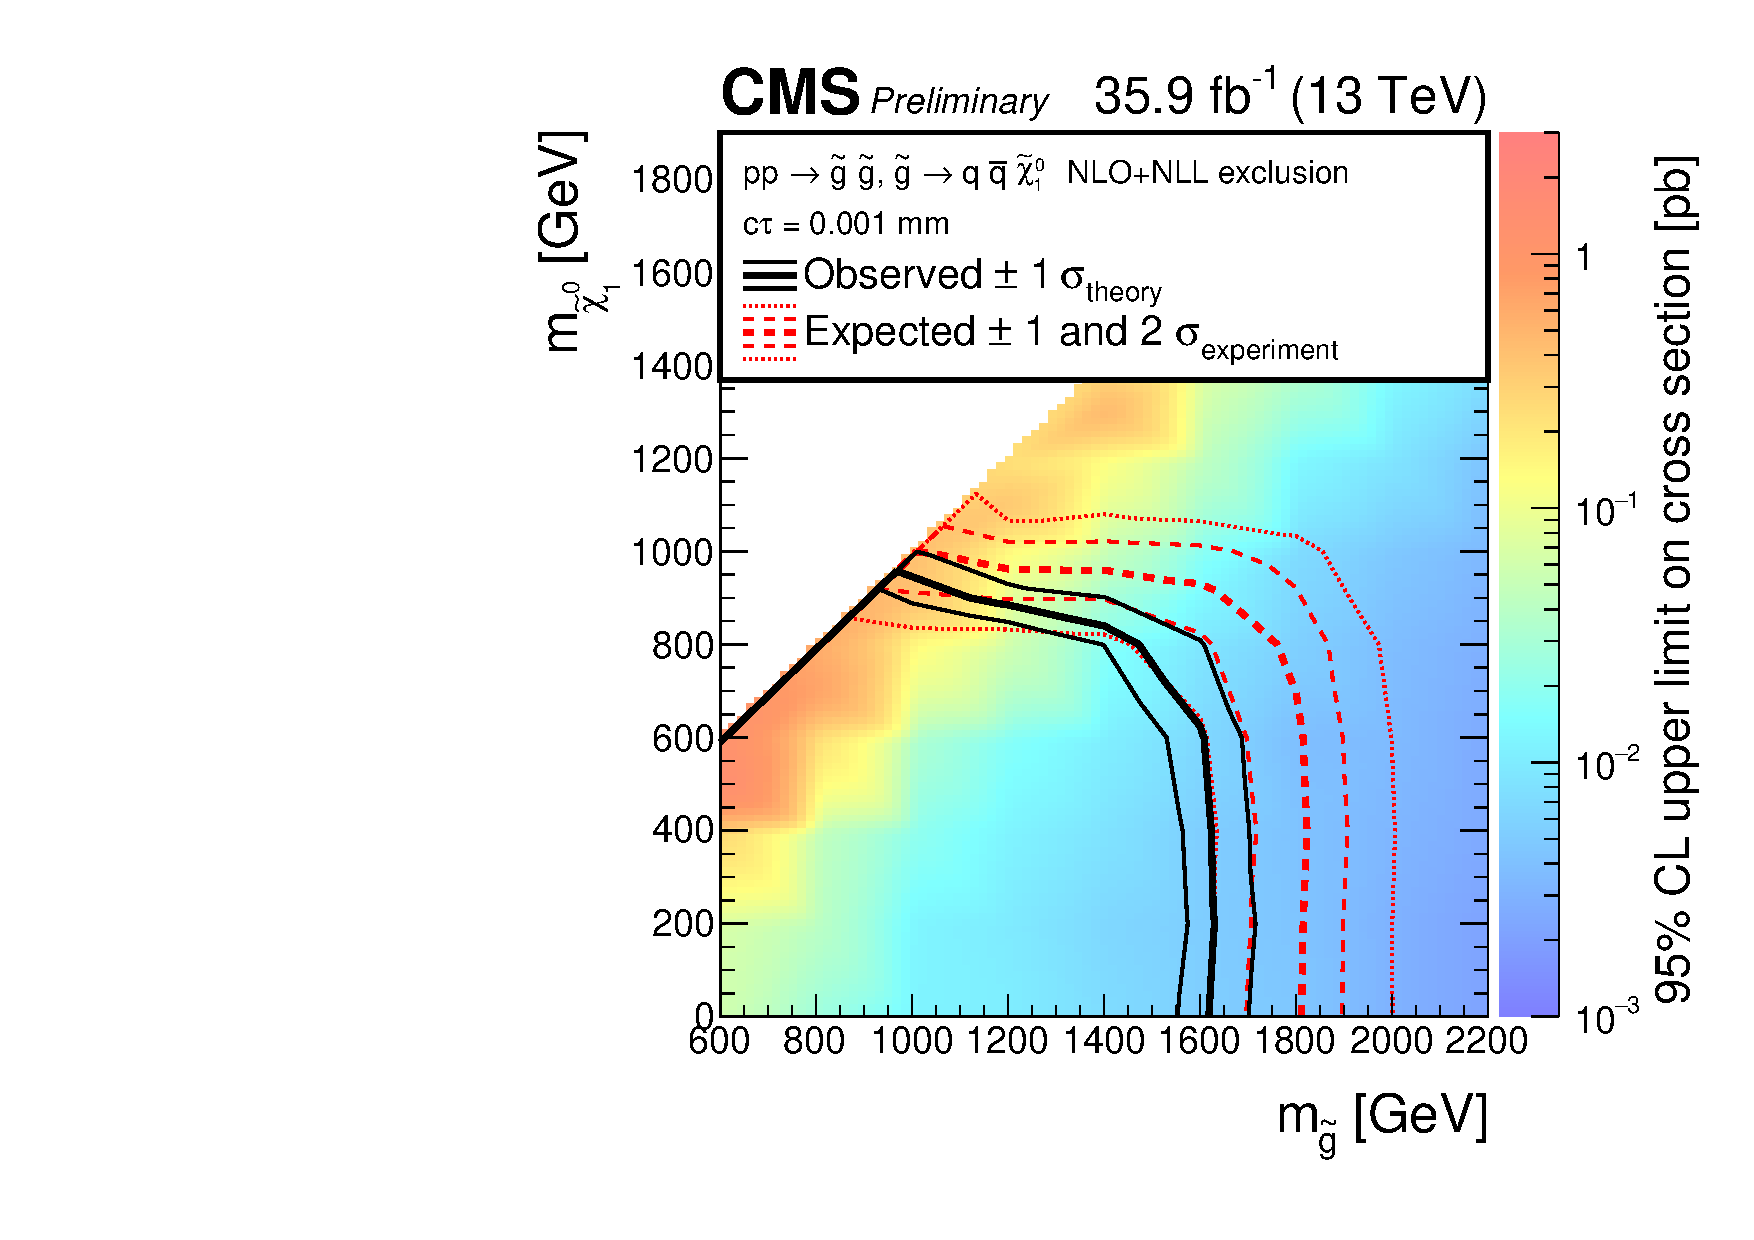
\includegraphics[width=0.6\textwidth]{figures/LLPResults/T1qqqqLL_ctau-0p001_XSEC}
            \label{fig:T1qqqqLL_excl_ctau-0p001}
        } \\
        \subfigure[T1qqqqLL ($\ctau = 0.001\unit{mm}$): $\epsilon_{sig}$]{
            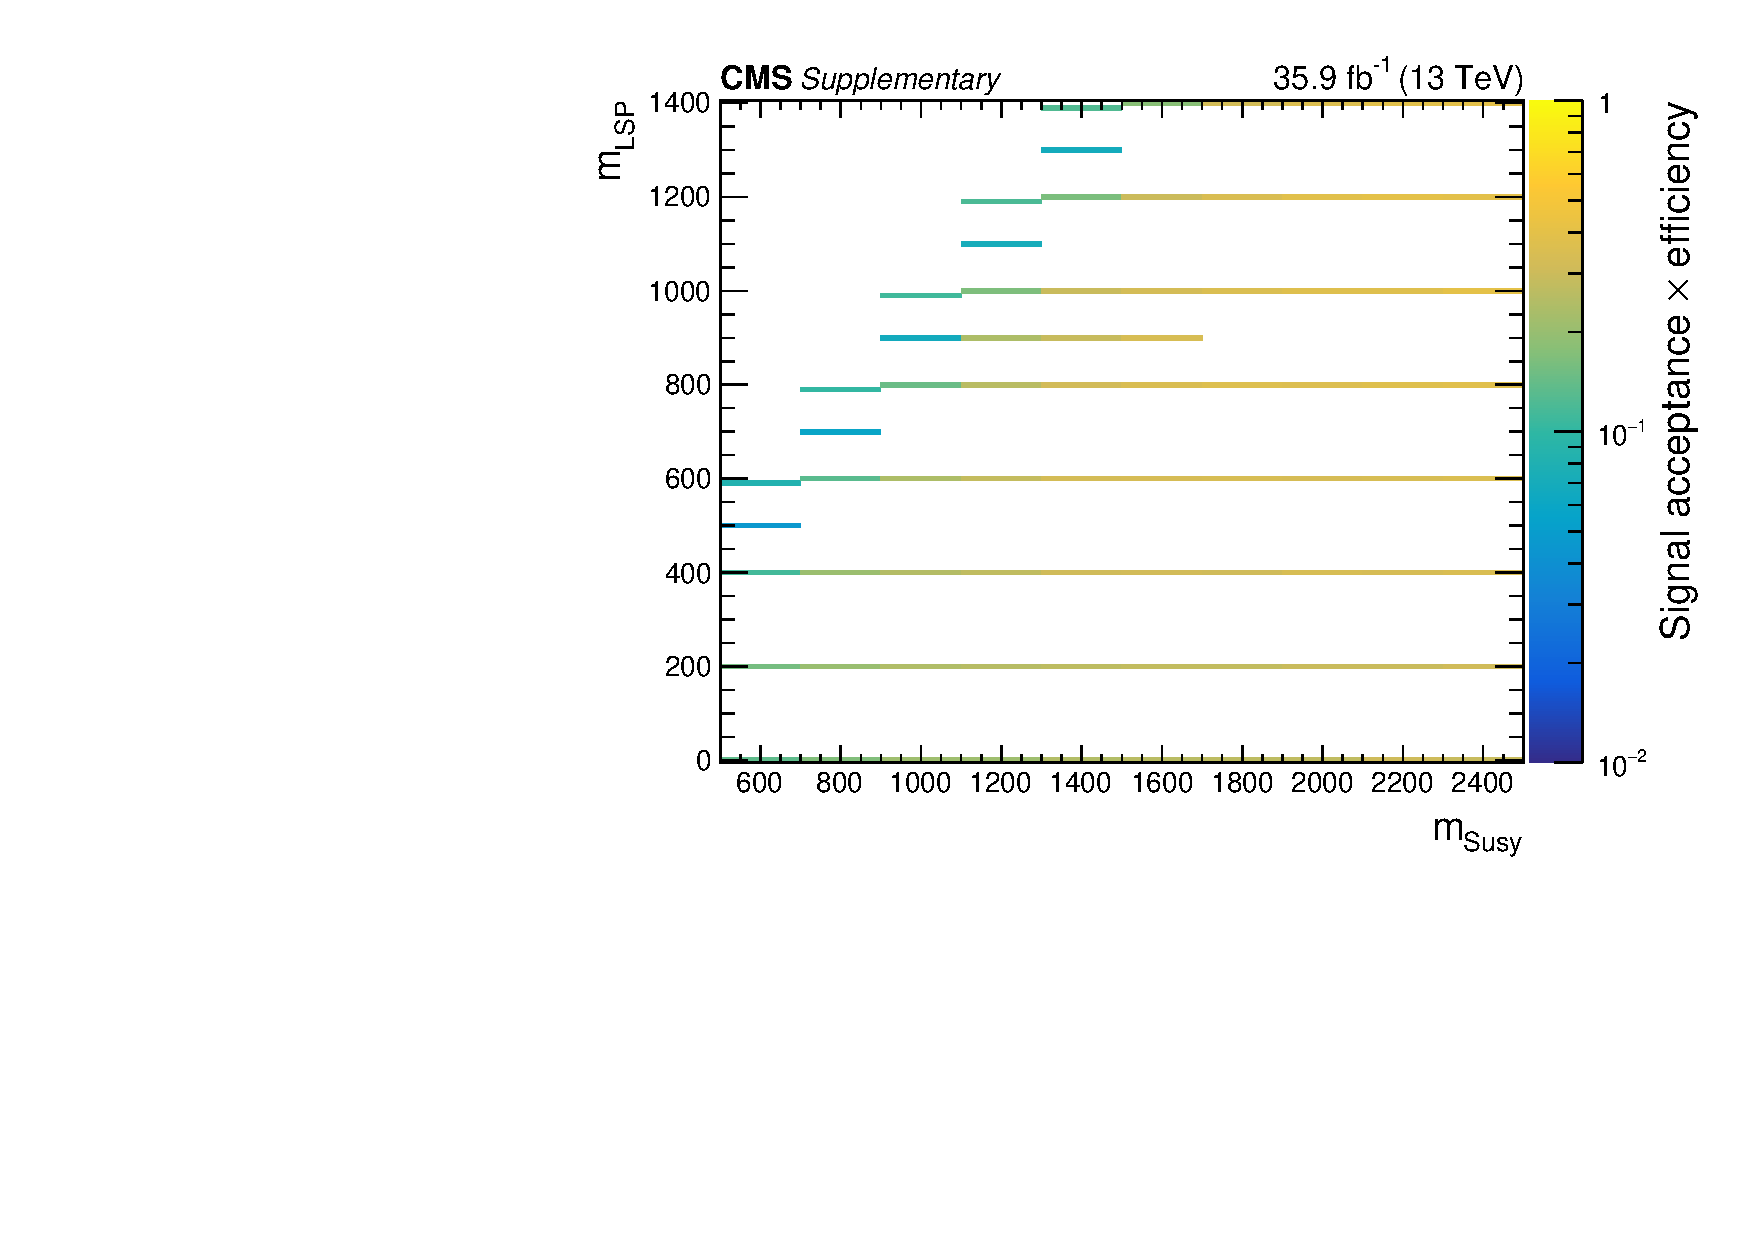
\includegraphics[width=0.45\textwidth]{figures/LLPResults/T1qqqqLL_ctau-0p001_effs}
            \label{fig:T1qqqqLL_eff_ctau-0p001}
        } ~~
        \subfigure[T1qqqqLL ($\ctau = 0.001\unit{mm}$): Most sensitive categories]{
            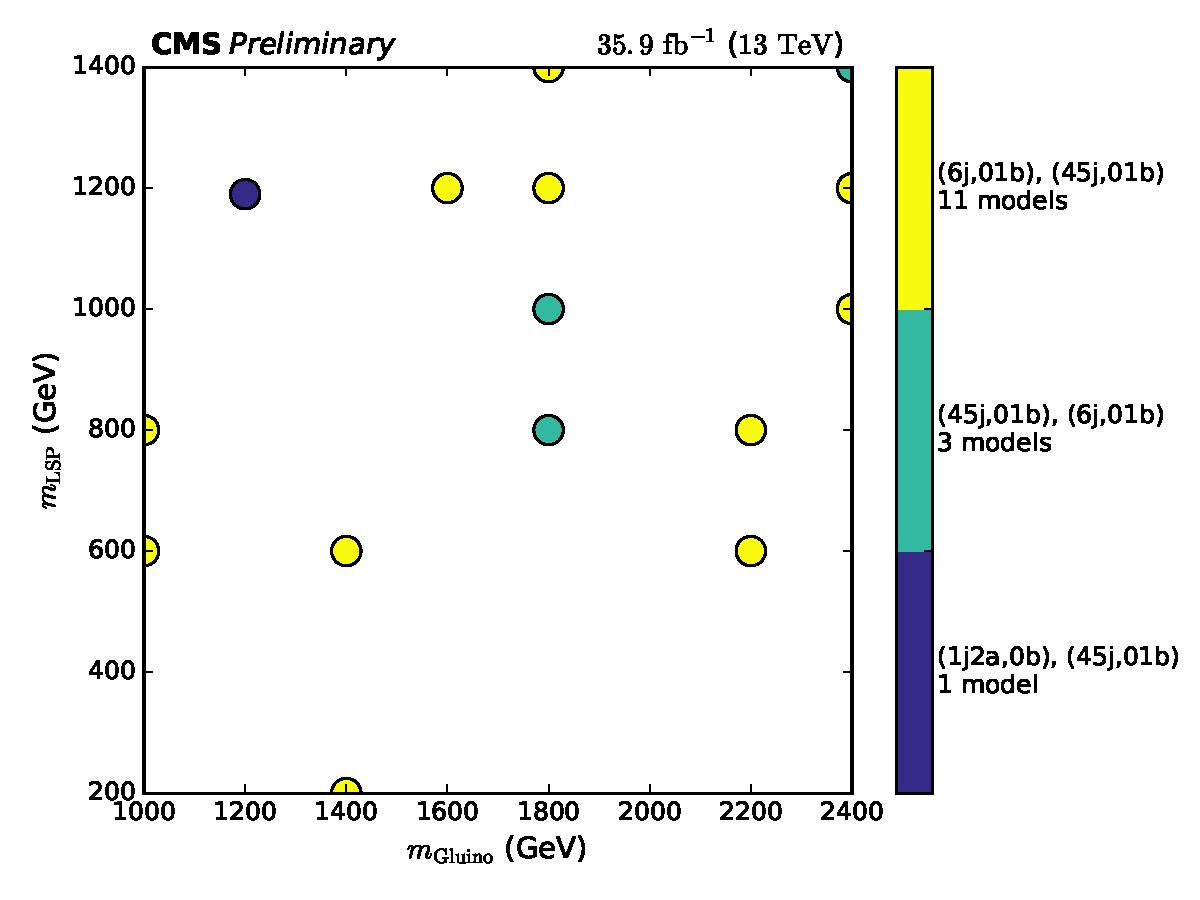
\includegraphics[width=0.45\textwidth]{figures/LLPResults/T1qqqqLL_ctau-0p001_bitMap}
            \label{fig:T1qqqqLL_bitMap_ctau-0p001}
        } \\
        %\subfigure[T1qqqqLL (\ctau = 1~mm): Significance scan]{
        %    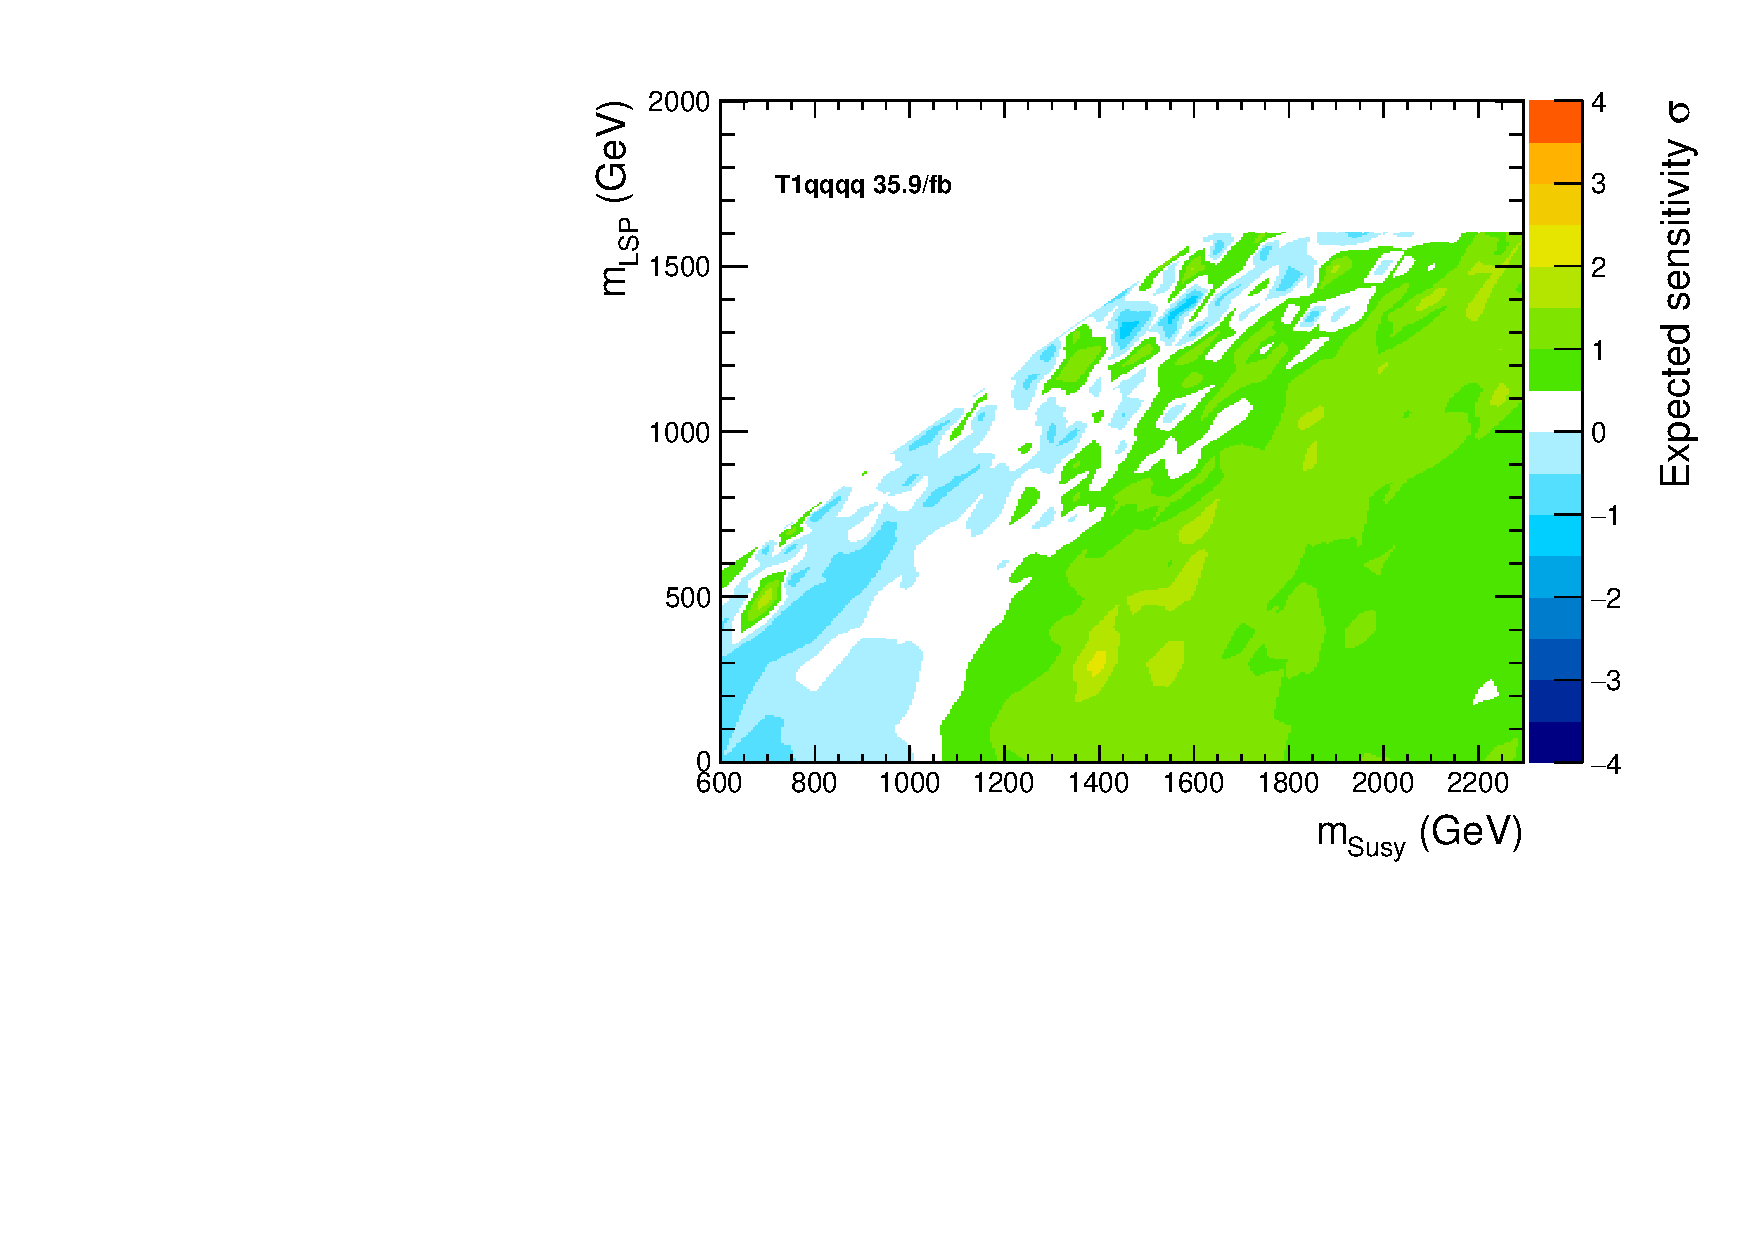
\includegraphics[width=0.45\linewidth]{figures/LLPResults/T1qqqqLL_ctau-1_signif}
        %    \label{fig:T1qqqqLL_signif}
        %} ~~
        \caption{Top: the 95\% C.L. observed upper limit on the cross section
            (histogram), with the expected (solid black line) observed
            (solid red line) exclusion contours. Left: signal acceptance
            including all jet categories. Right: graph showing the most 
            sensitive event topologies for each mass point.
            %Bottom: local observed significance scan.
        }
        \label{fig:T1qqqqLL:ctau-0p001}
    \end{center}
\end{figure}

\newpage
\begin{figure}[h!]
    \begin{center}
        \subfigure[T1qqqqLL ($\ctau = 0.01\unit{mm}$): Upper limit on the cross section in the mass plane]{
            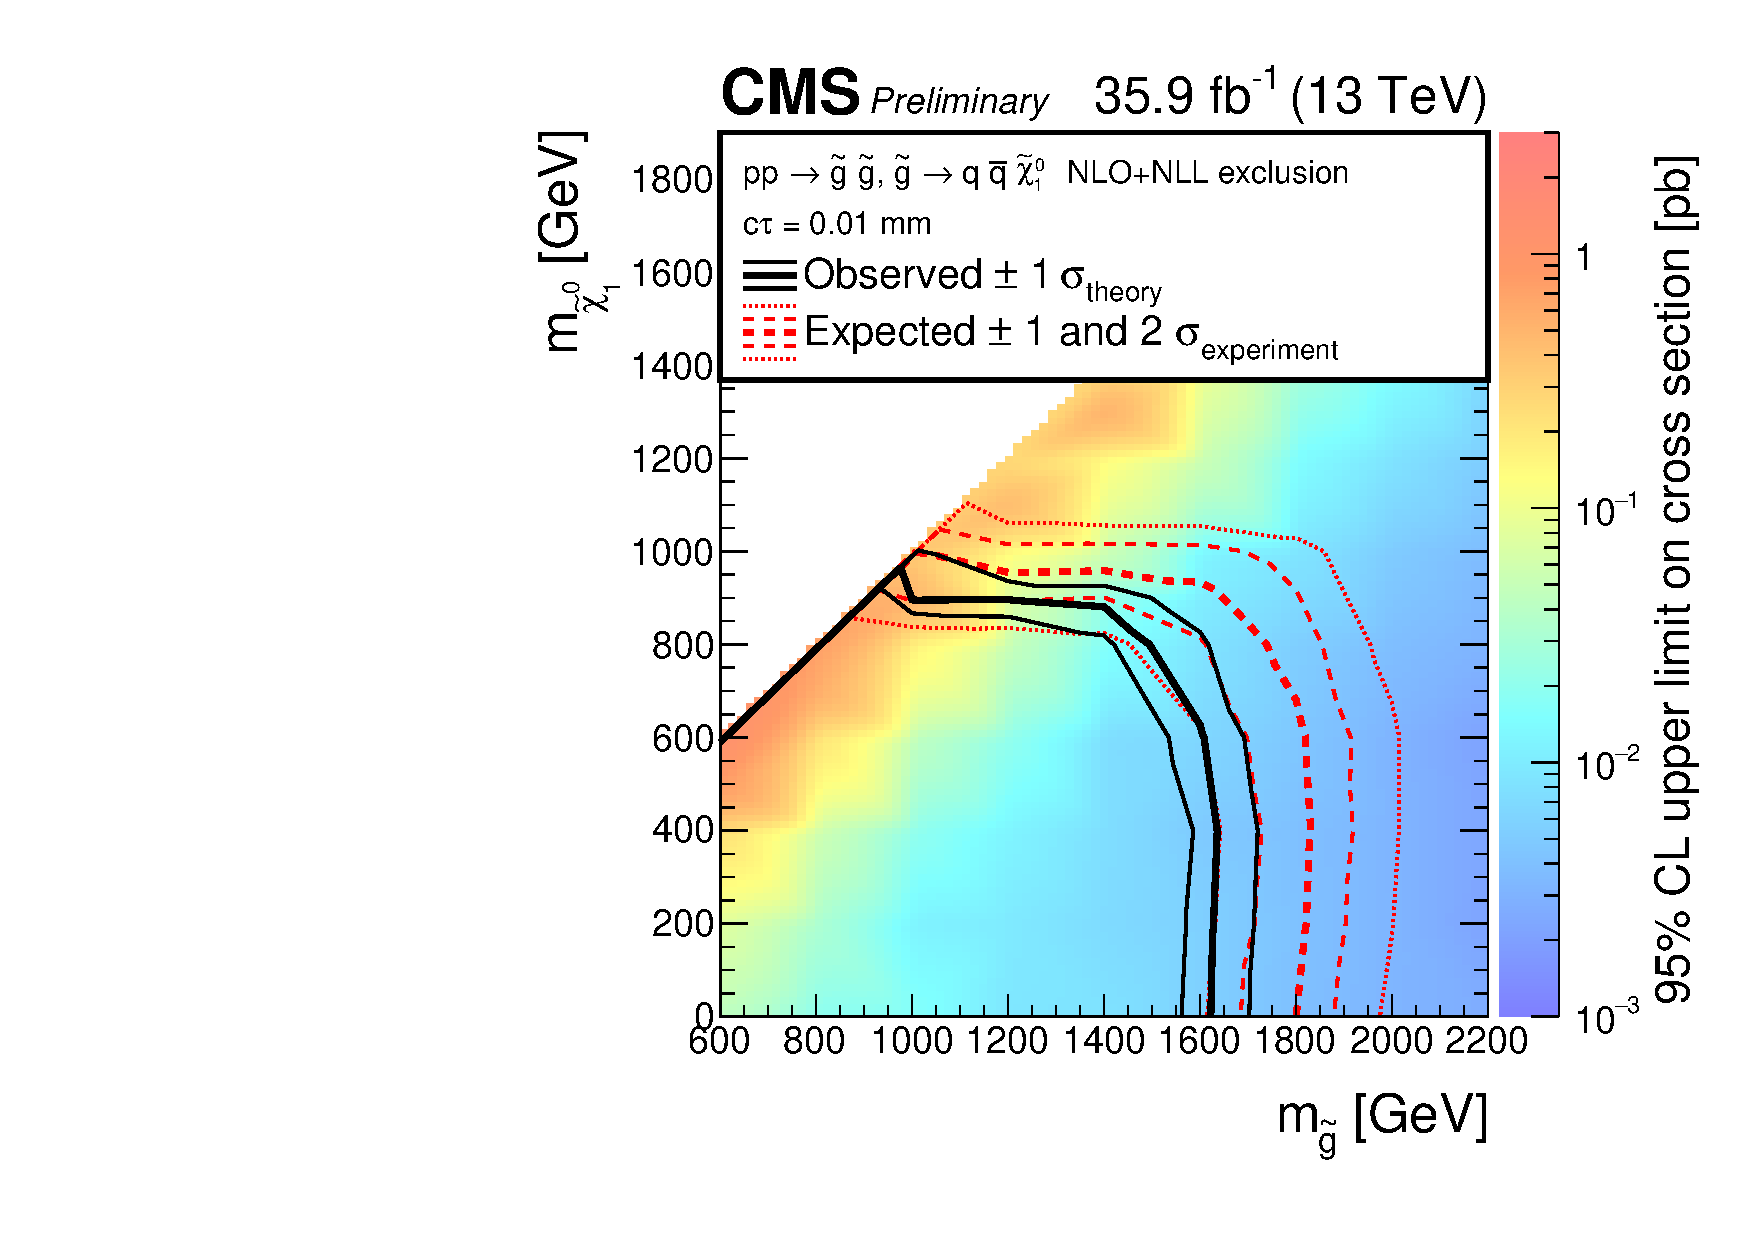
\includegraphics[width=0.6\textwidth]{figures/LLPResults/T1qqqqLL_ctau-0p01_XSEC}
            \label{fig:T1qqqqLL_excl_ctau-0p01}
        } \\
        \subfigure[T1qqqqLL ($\ctau = 0.01\unit{mm}$): $\epsilon_{sig}$]{
            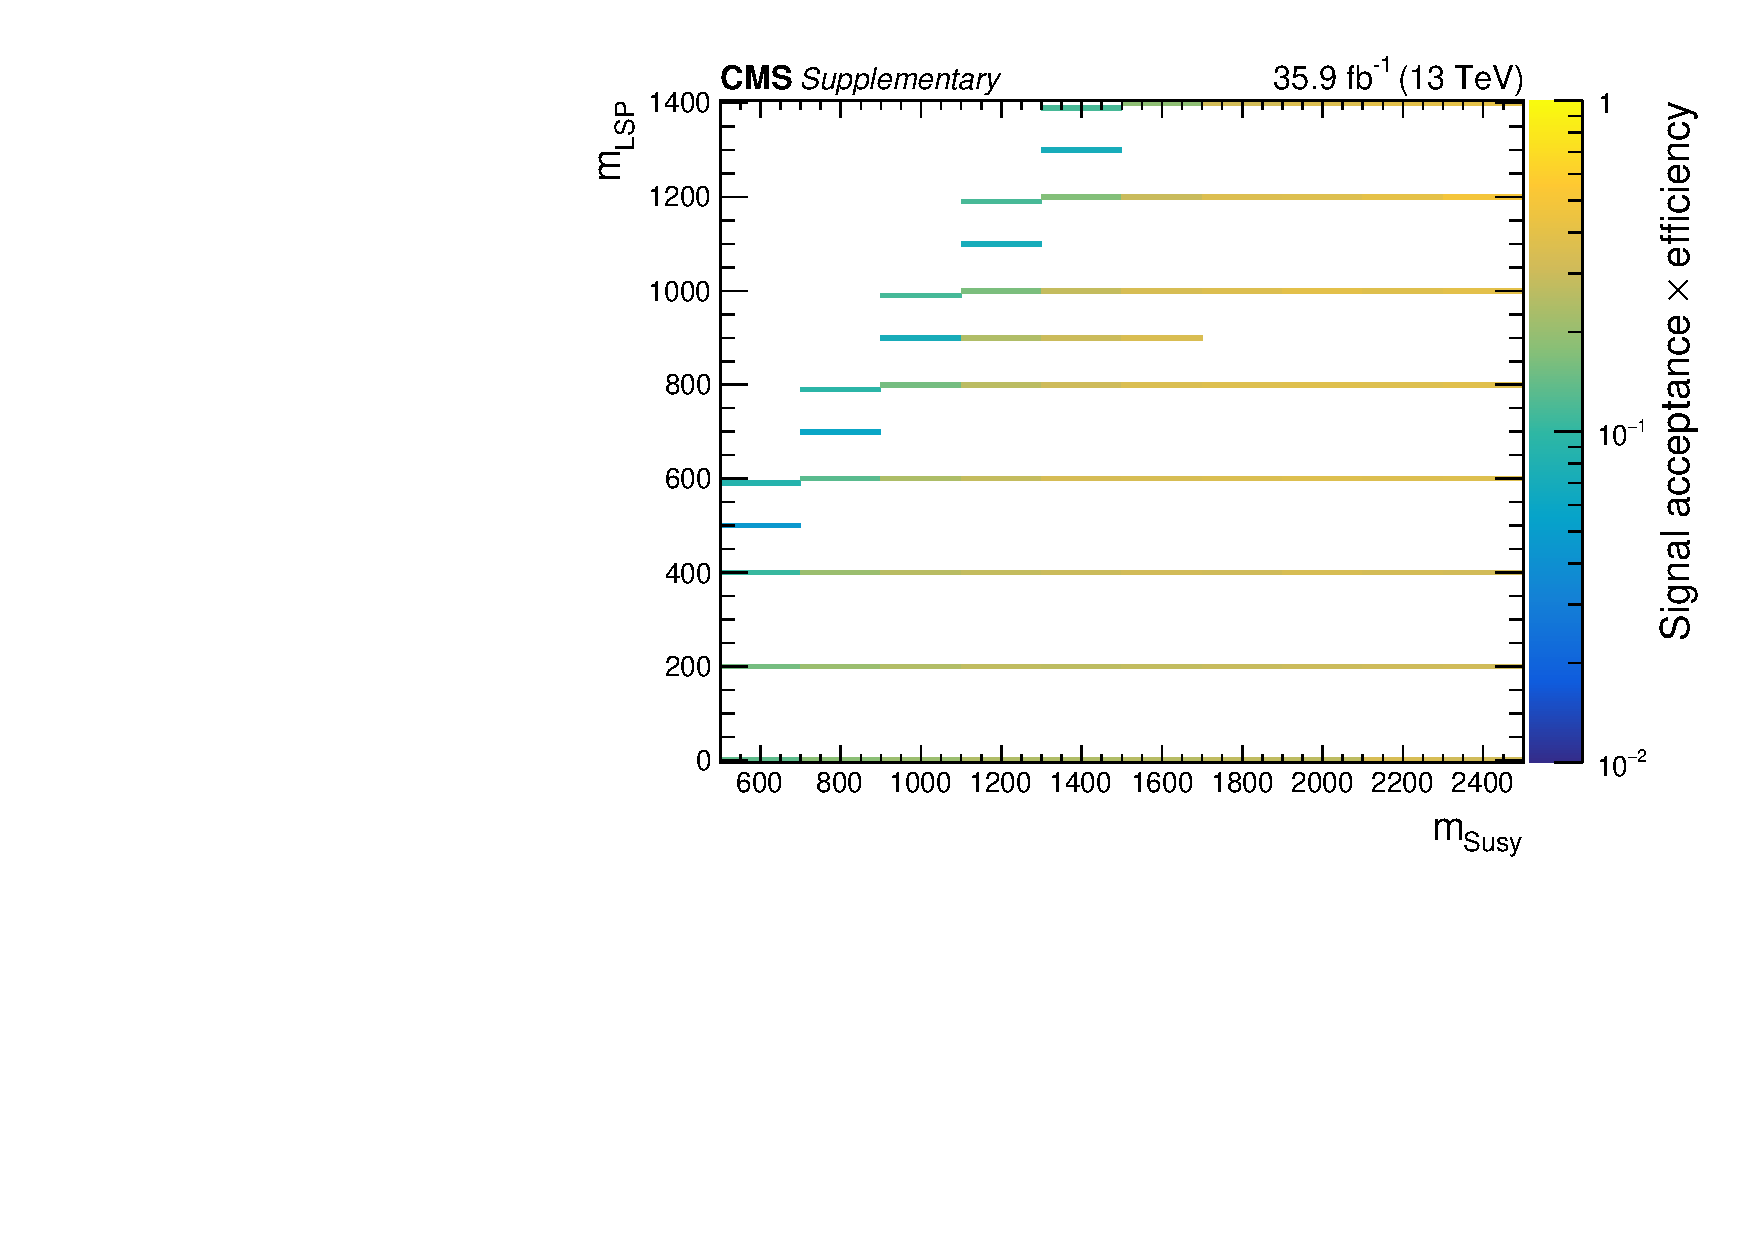
\includegraphics[width=0.45\textwidth]{figures/LLPResults/T1qqqqLL_ctau-0p01_effs}
            \label{fig:T1qqqqLL_eff_ctau-0p01}
        } ~~
        \subfigure[T1qqqqLL ($\ctau = 0.01\unit{mm}$): Most sensitive categories]{
            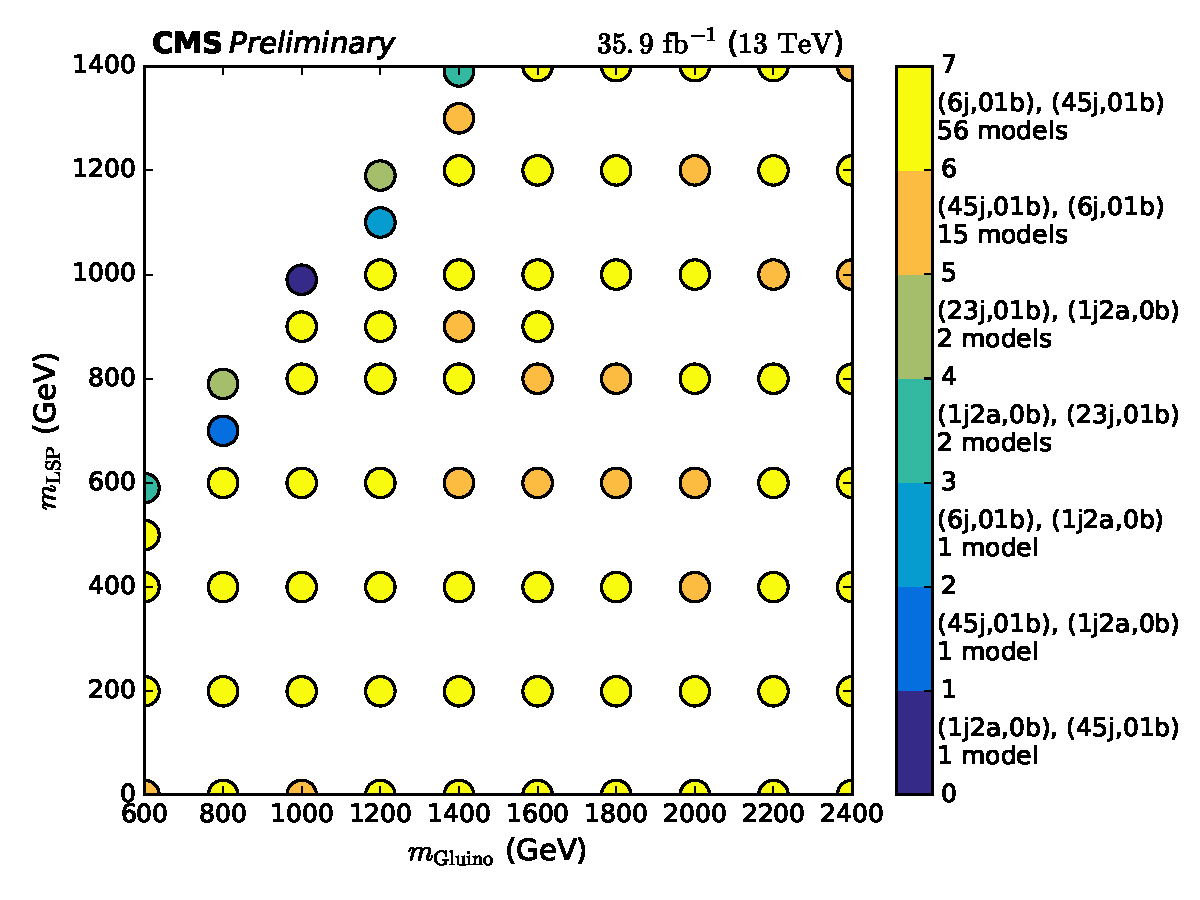
\includegraphics[width=0.45\textwidth]{figures/LLPResults/T1qqqqLL_ctau-0p01_bitMap}
            \label{fig:T1qqqqLL_bitMap_ctau-0p01}
        } \\
        %\subfigure[T1qqqqLL (\ctau = 1~mm): Significance scan]{
        %    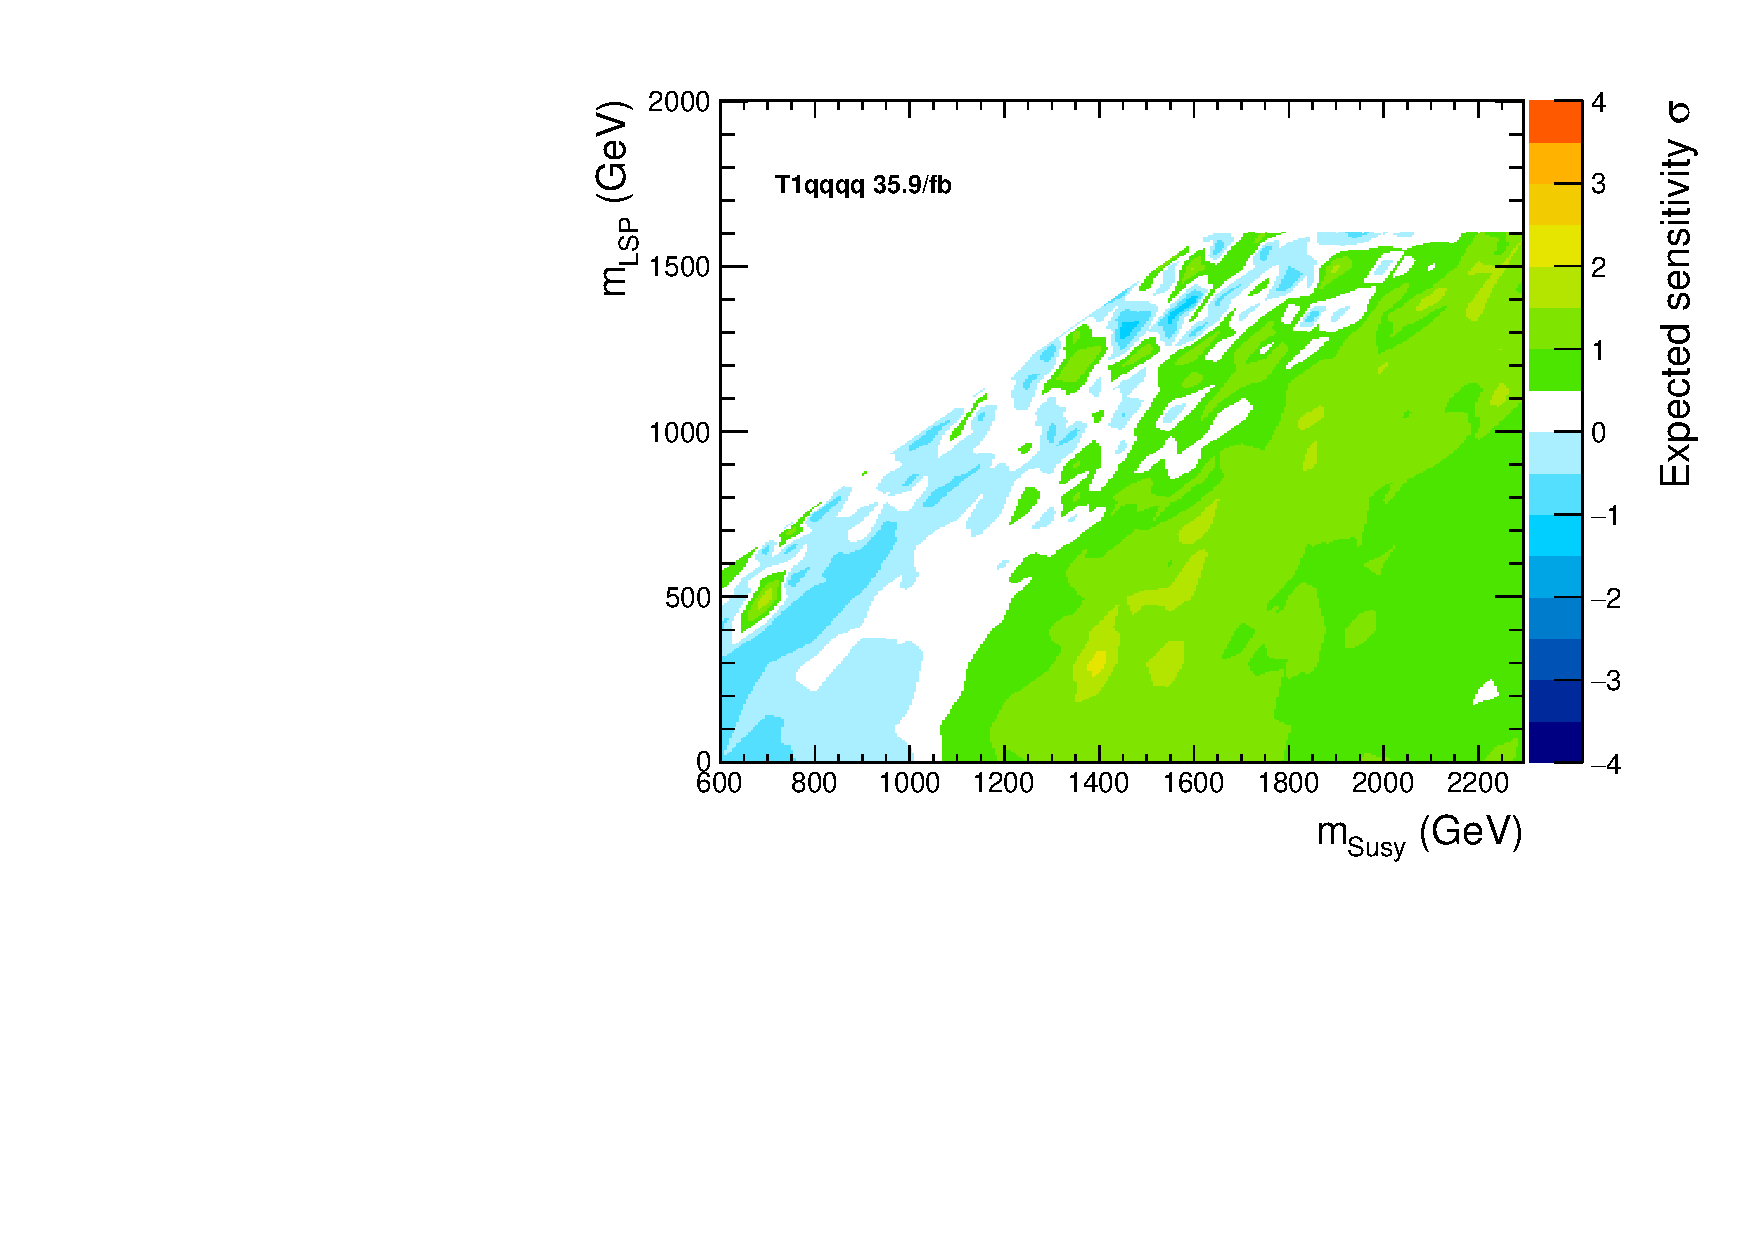
\includegraphics[width=0.45\linewidth]{figures/LLPResults/T1qqqqLL_ctau-1_signif}
        %    \label{fig:T1qqqqLL_signif}
        %} ~~
        \caption{Top: the 95\% C.L. observed upper limit on the cross section
            (histogram), with the expected (solid black line) observed
            (solid red line) exclusion contours. Left: signal acceptance
            including all jet categories. Right: graph showing the most 
            sensitive event topologies for each mass point.
            %Bottom: local observed significance scan.
        }
        \label{fig:T1qqqqLL:ctau-0p01}
    \end{center}
\end{figure}

\newpage
\begin{figure}[h!]
    \begin{center}
        \subfigure[T1qqqqLL ($\ctau = 0.1\unit{mm}$): Upper limit on the cross section in the mass plane]{
            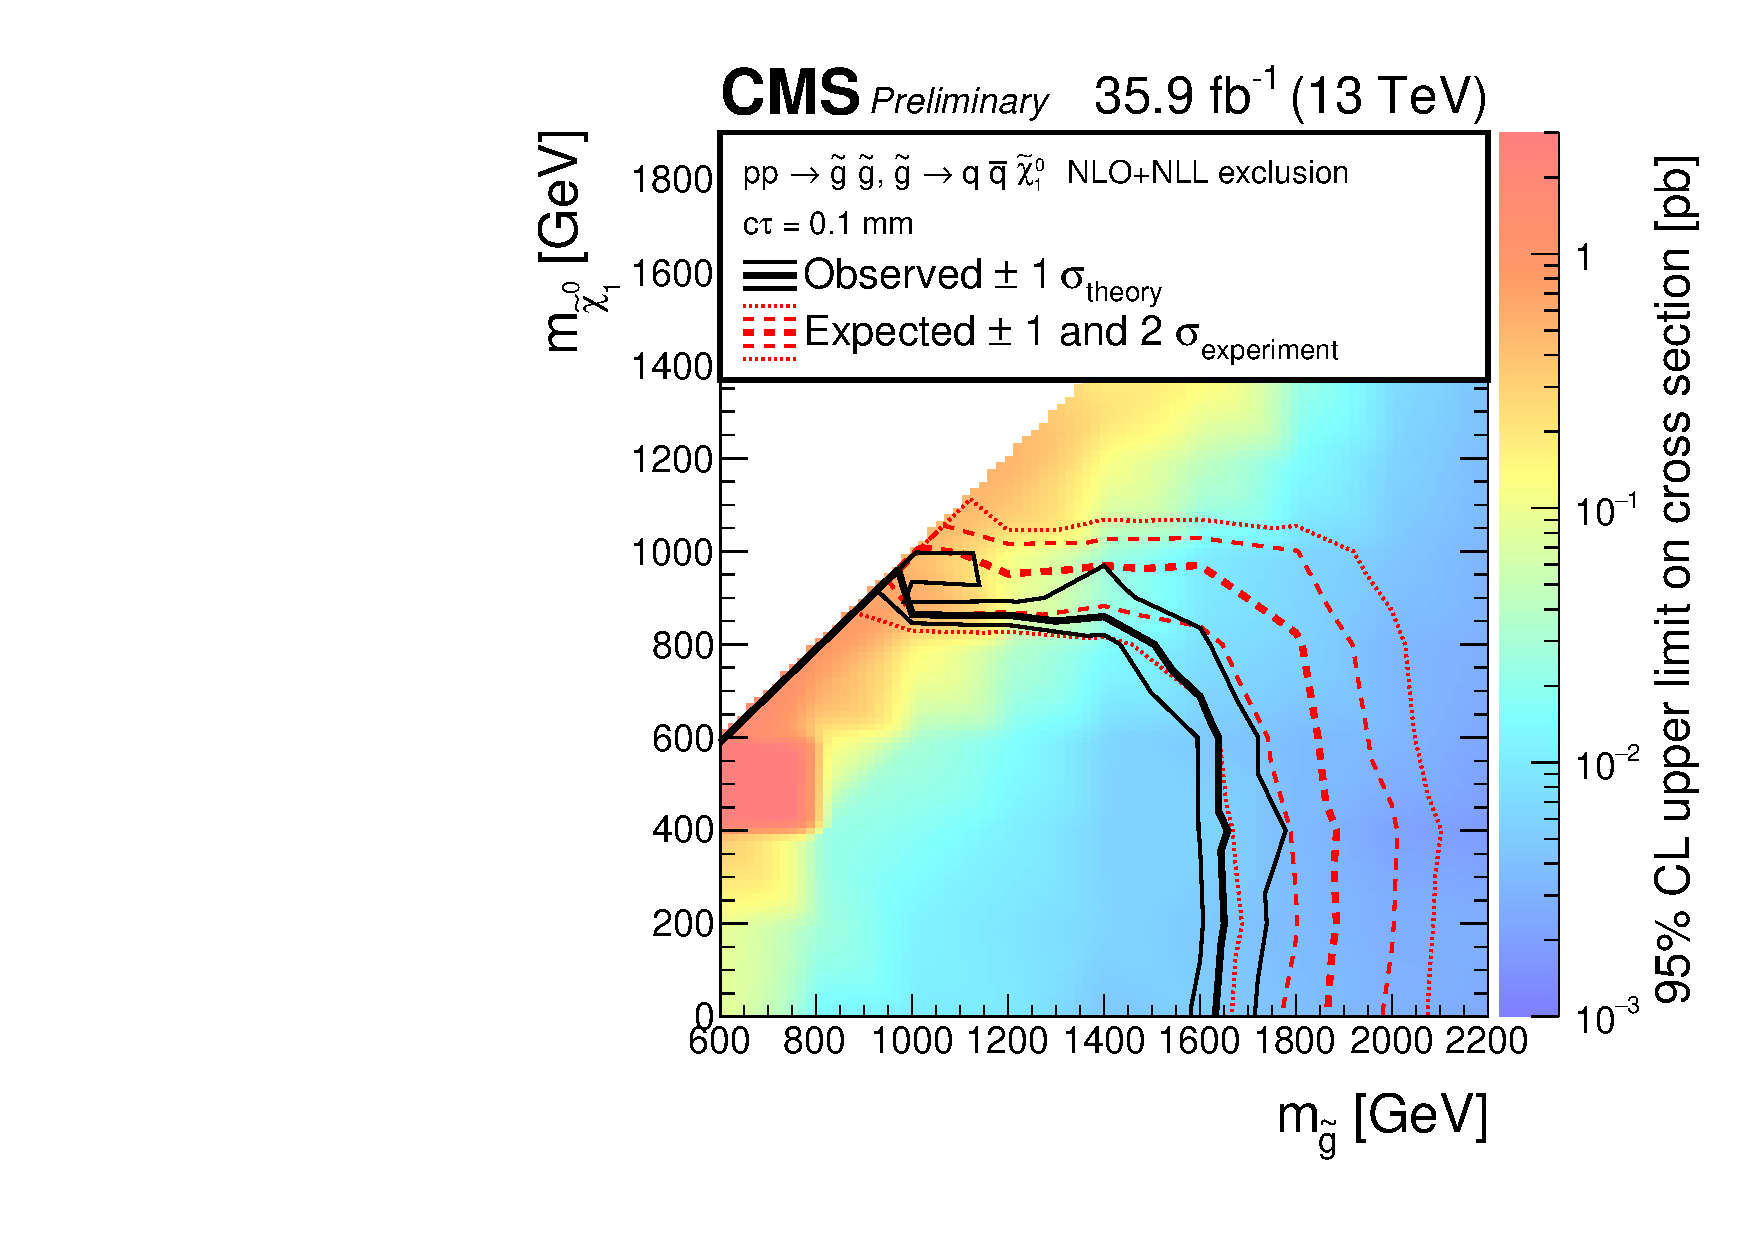
\includegraphics[width=0.6\textwidth]{figures/LLPResults/T1qqqqLL_ctau-0p1_XSEC}
            \label{fig:T1qqqqLL_excl_ctau-0p1}
        } \\
        \subfigure[T1qqqqLL ($\ctau = 0.1\unit{mm}$): $\epsilon_{sig}$]{
            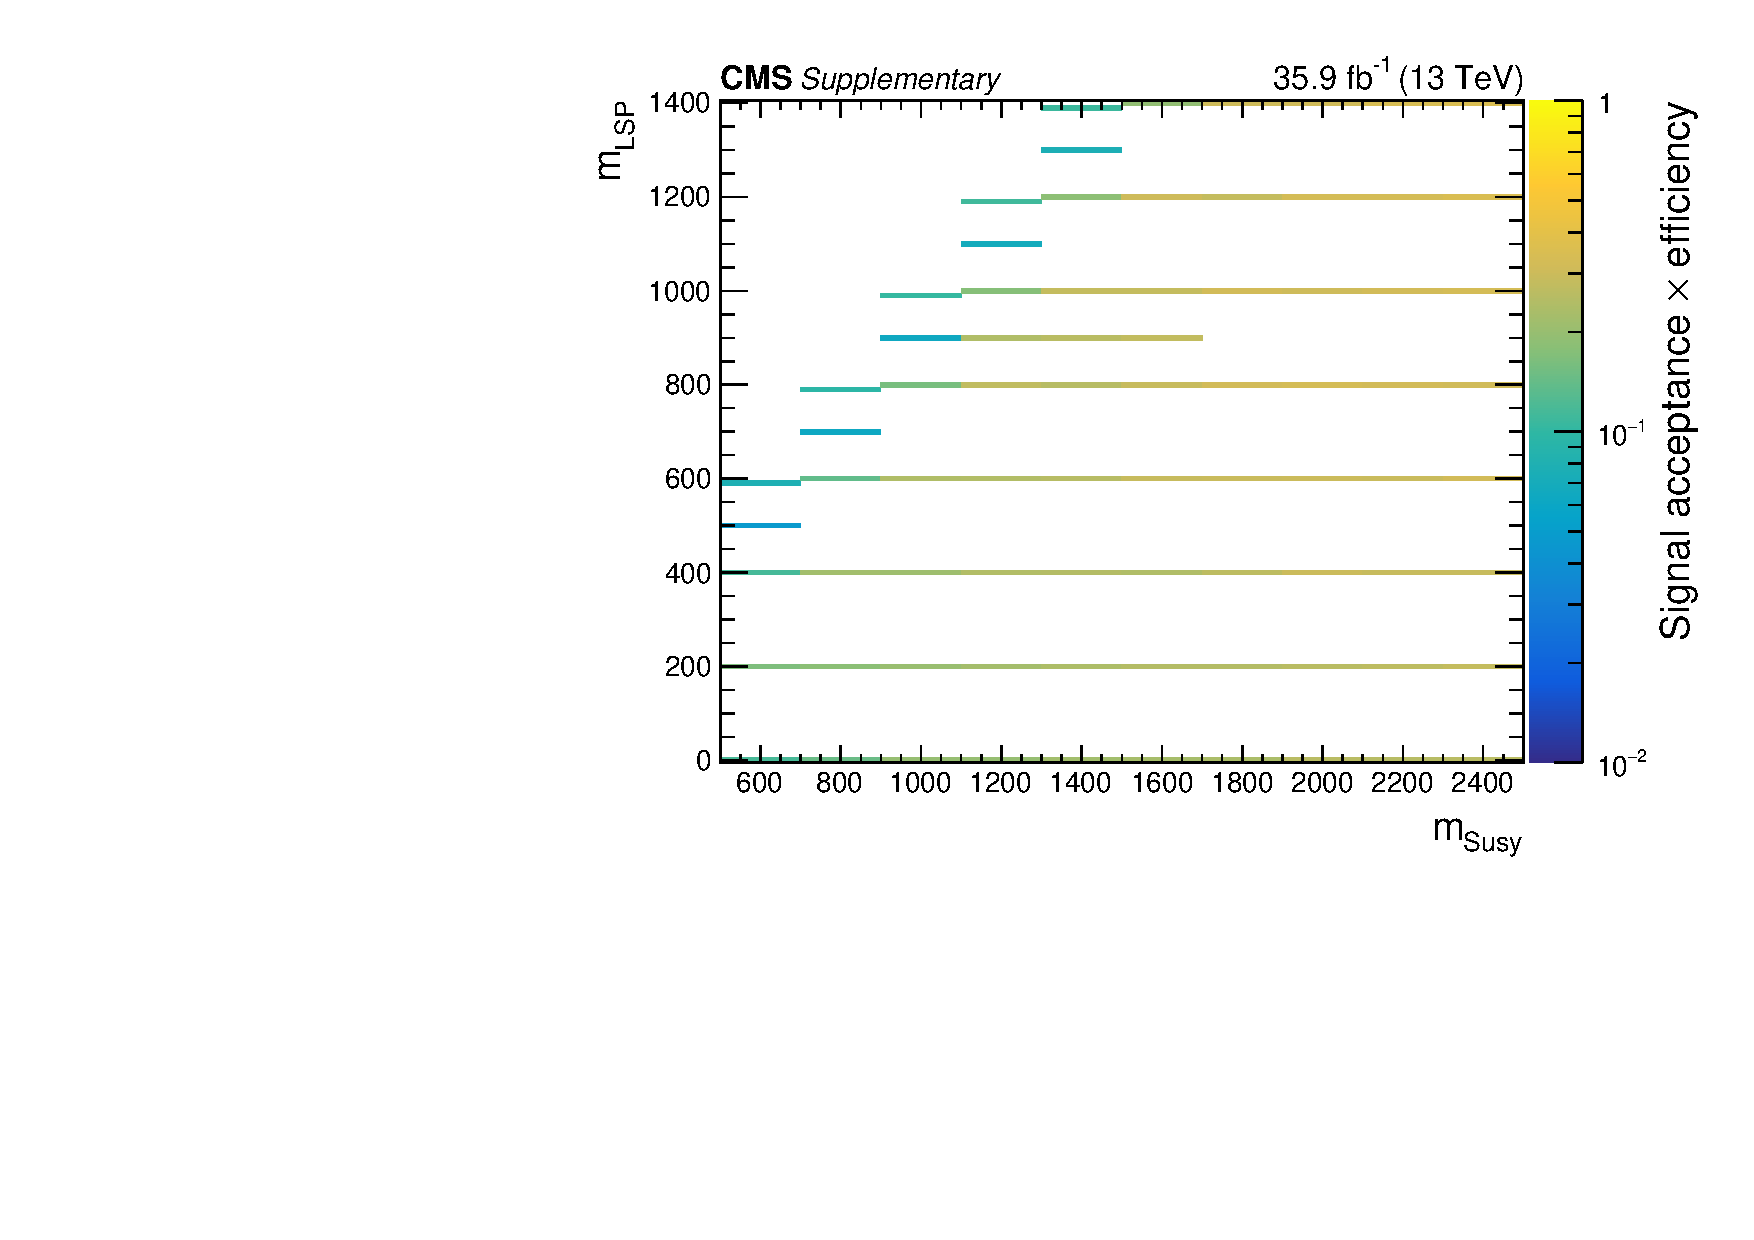
\includegraphics[width=0.45\textwidth]{figures/LLPResults/T1qqqqLL_ctau-0p1_effs}
            \label{fig:T1qqqqLL_eff_ctau-0p1}
        } ~~
        \subfigure[T1qqqqLL ($\ctau = 0.1\unit{mm}$): Most sensitive categories]{
            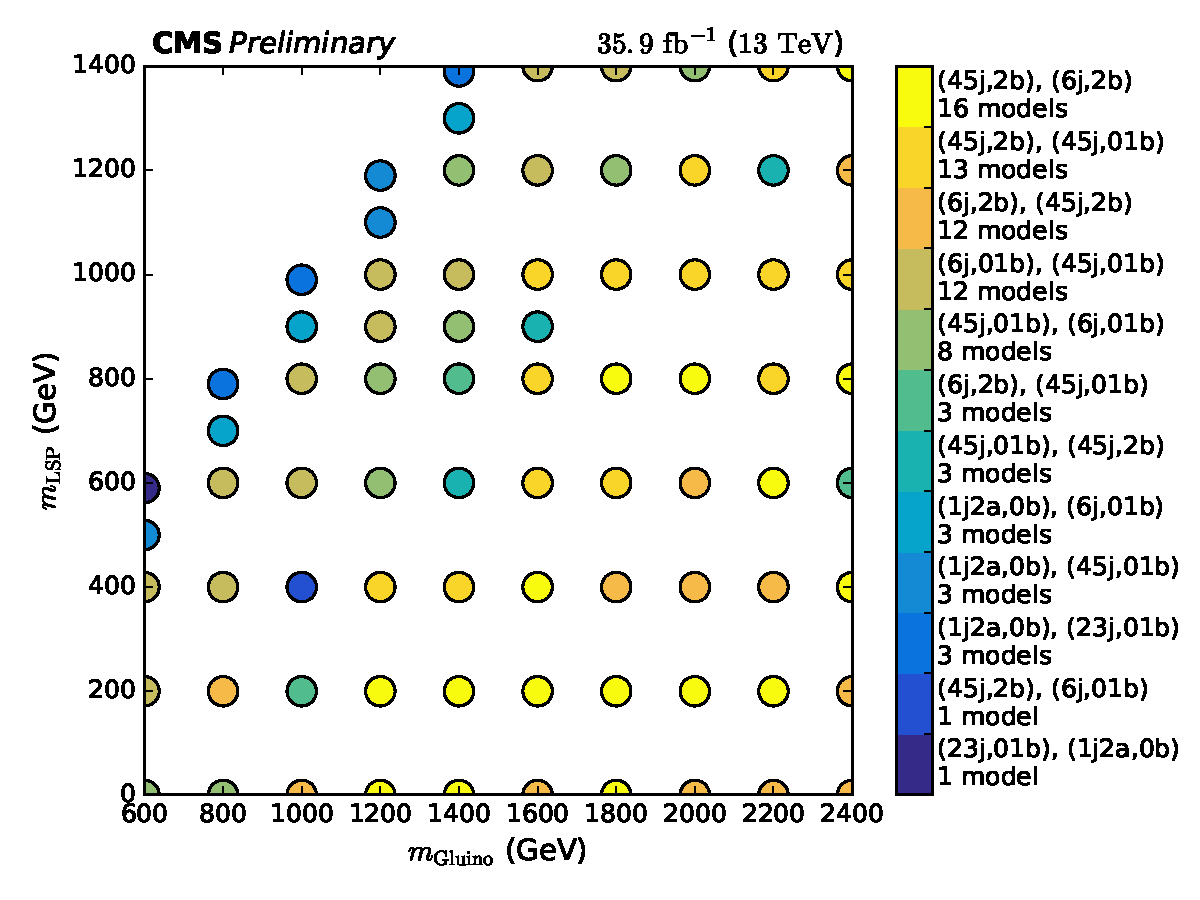
\includegraphics[width=0.45\textwidth]{figures/LLPResults/T1qqqqLL_ctau-0p1_bitMap}
            \label{fig:T1qqqqLL_bitMap_ctau-0p1}
        } \\
        %\subfigure[T1qqqqLL ($\ctau = 1\unit{mm}$): Significance scan]{
        %    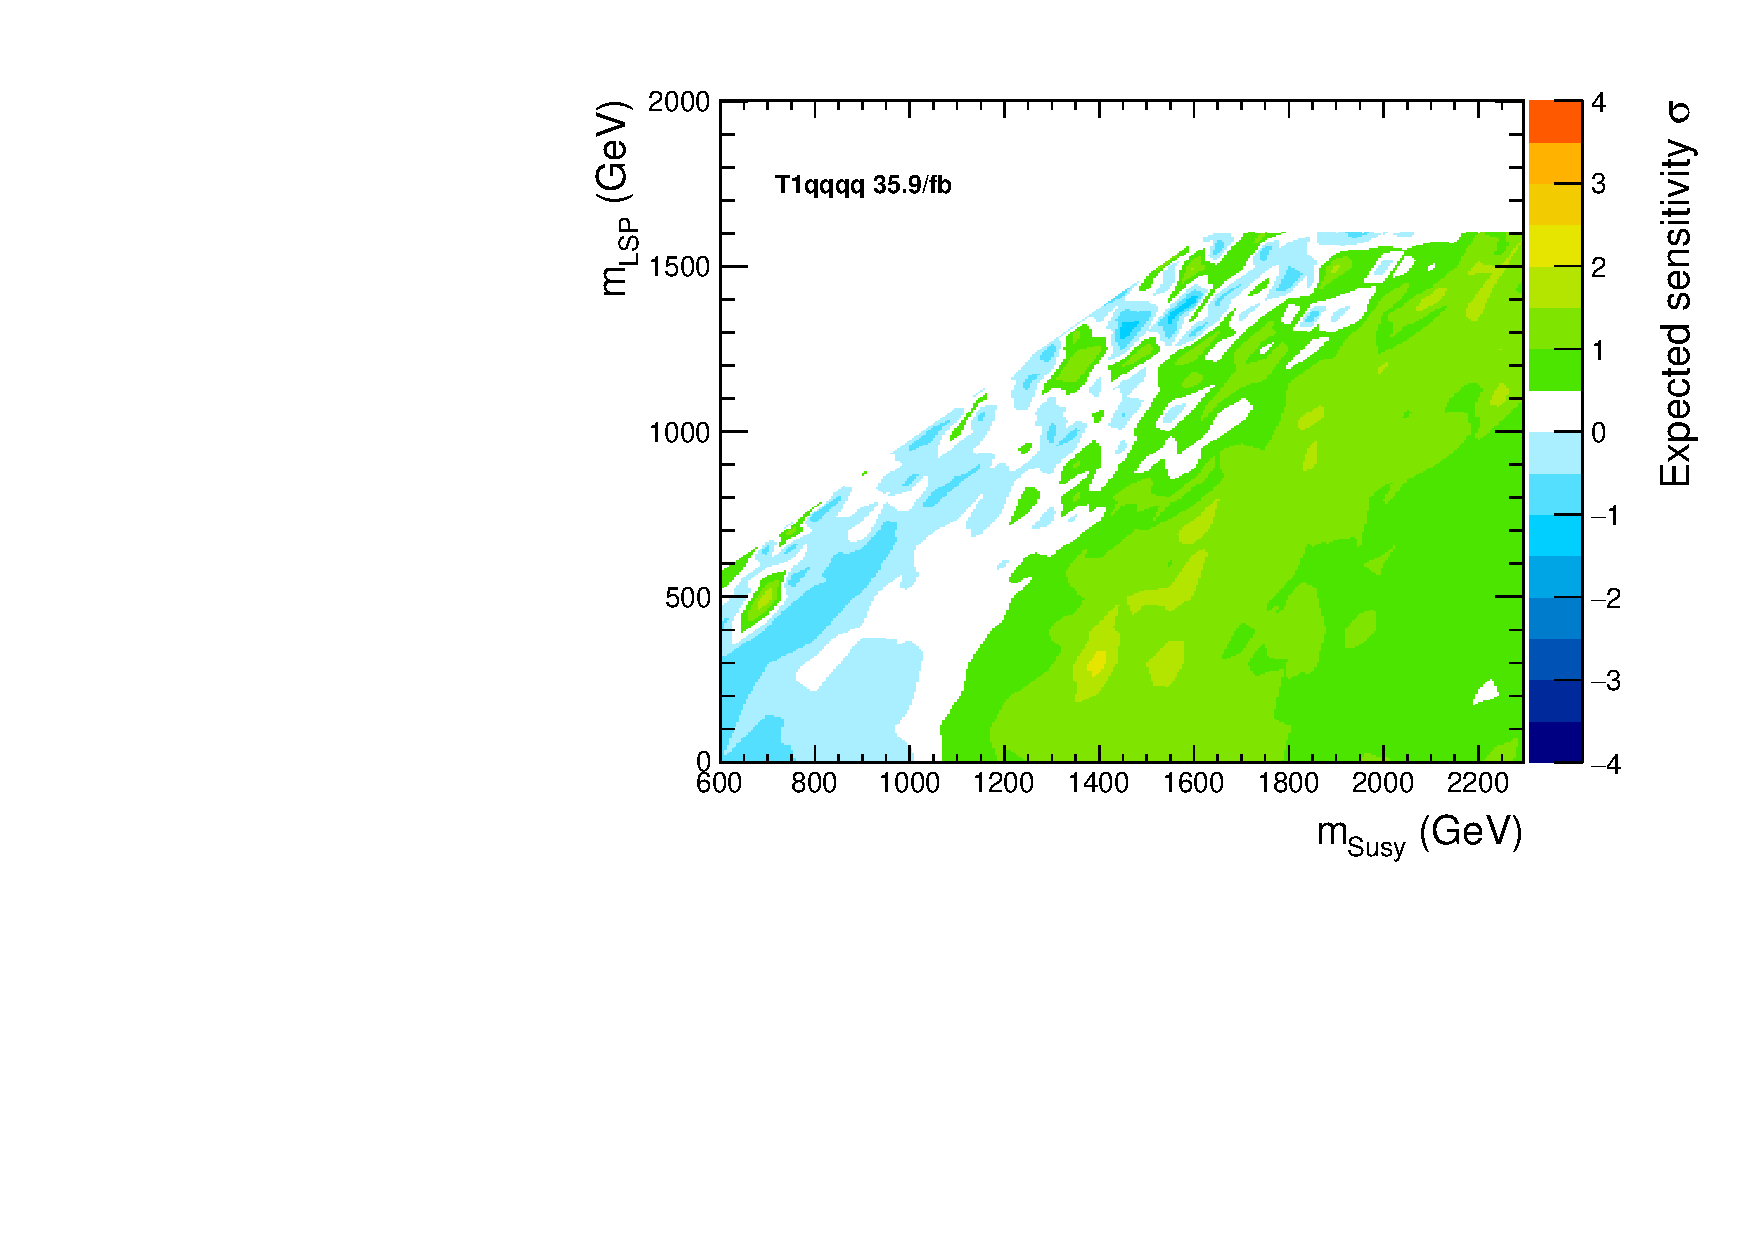
\includegraphics[width=0.45\linewidth]{figures/LLPResults/T1qqqqLL_ctau-1_signif}
        %    \label{fig:T1qqqqLL_signif_ctau-0p1}
        %} ~~
        \caption{Top: the 95\% C.L. observed upper limit on the cross section
            (histogram), with the expected (solid black line) observed
            (solid red line) exclusion contours. Left: signal acceptance
            including all jet categories. Right: graph showing the most 
            sensitive event topologies for each mass point.
            %Bottom: local observed significance scan.
        }
        \label{fig:T1qqqqLL:ctau-0p1}
    \end{center}
\end{figure}

\newpage
\begin{figure}[h!]
    \begin{center}
        \subfigure[T1qqqqLL ($\ctau = 1\unit{mm}$): Upper limit on the cross section in the mass plane]{
            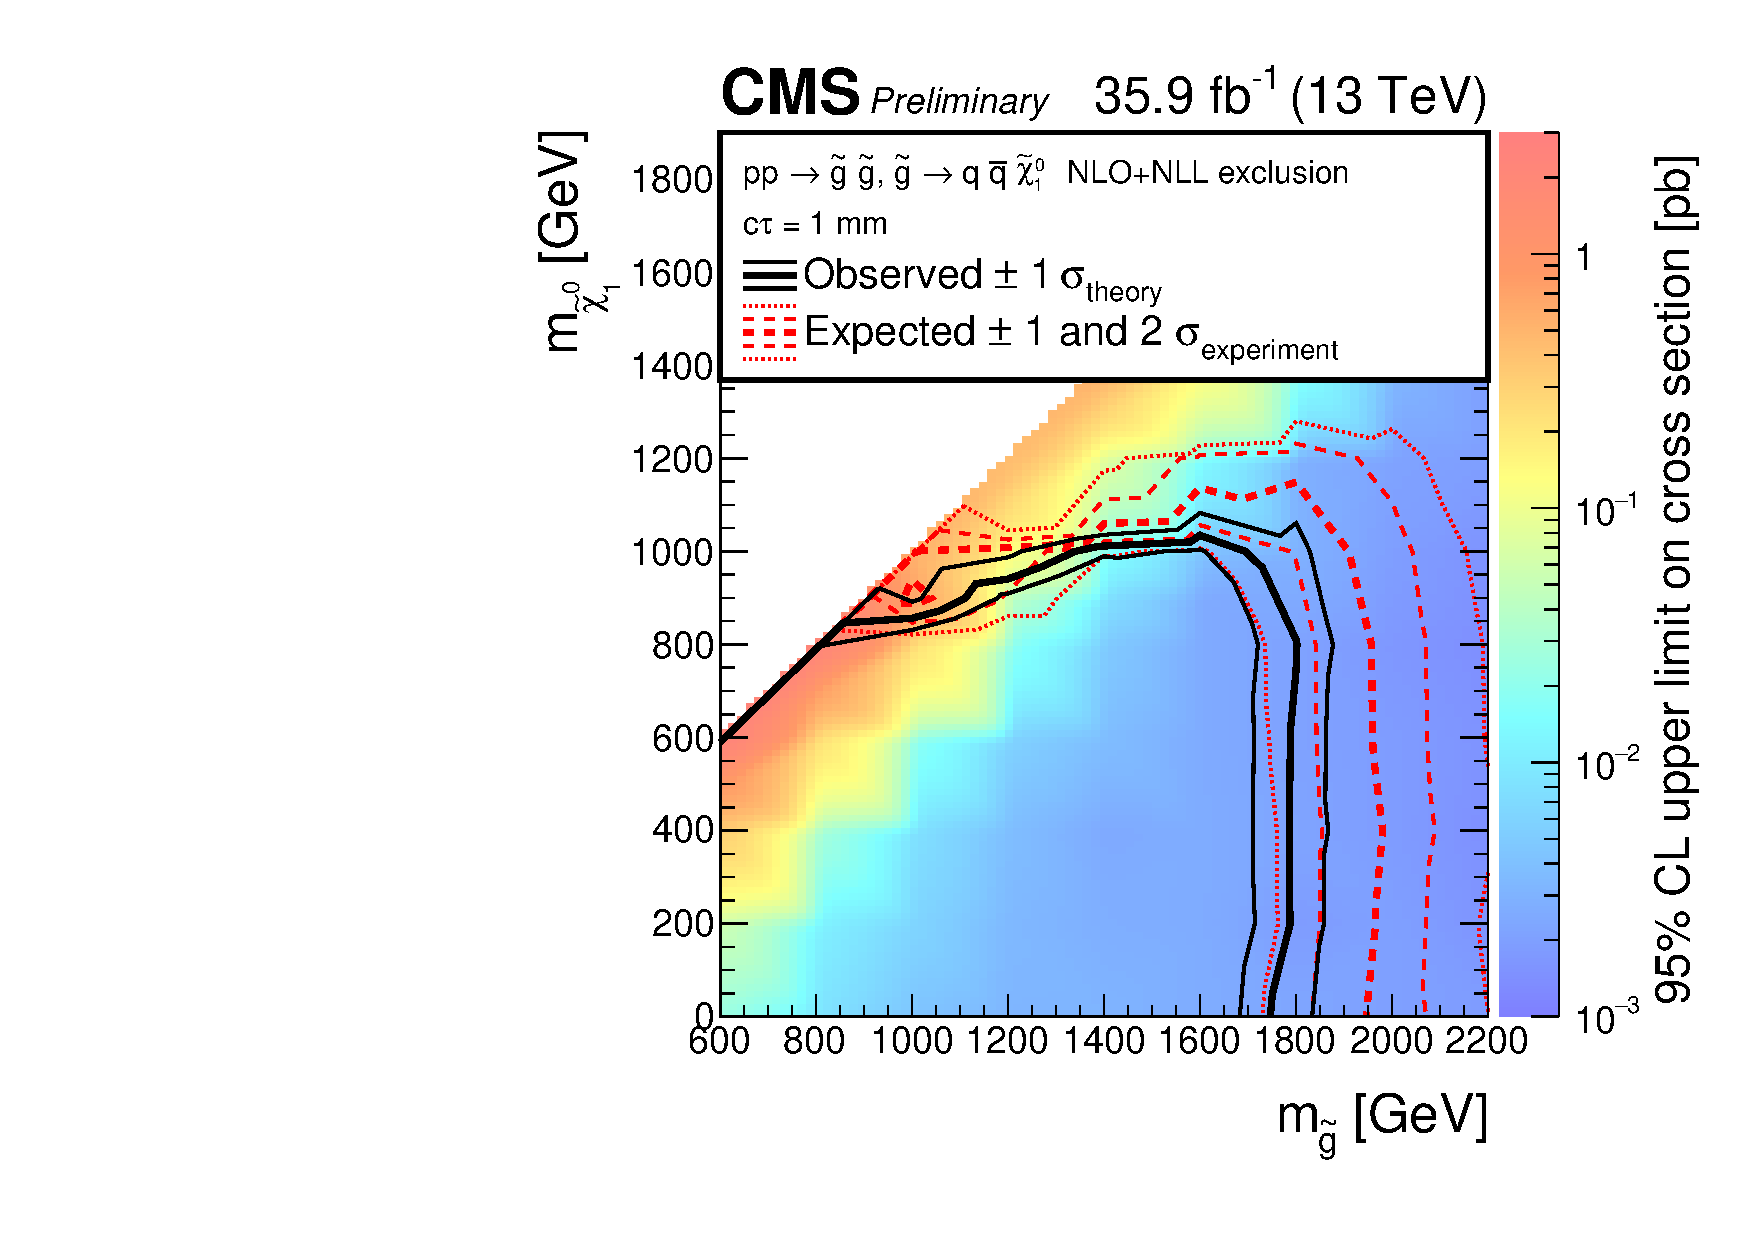
\includegraphics[width=0.6\textwidth]{figures/LLPResults/T1qqqqLL_ctau-1_XSEC}
            \label{fig:T1qqqqLL_excl_ctau-1}
        } \\
        \subfigure[T1qqqqLL ($\ctau = 1\unit{mm}$): $\epsilon_{sig}$]{
            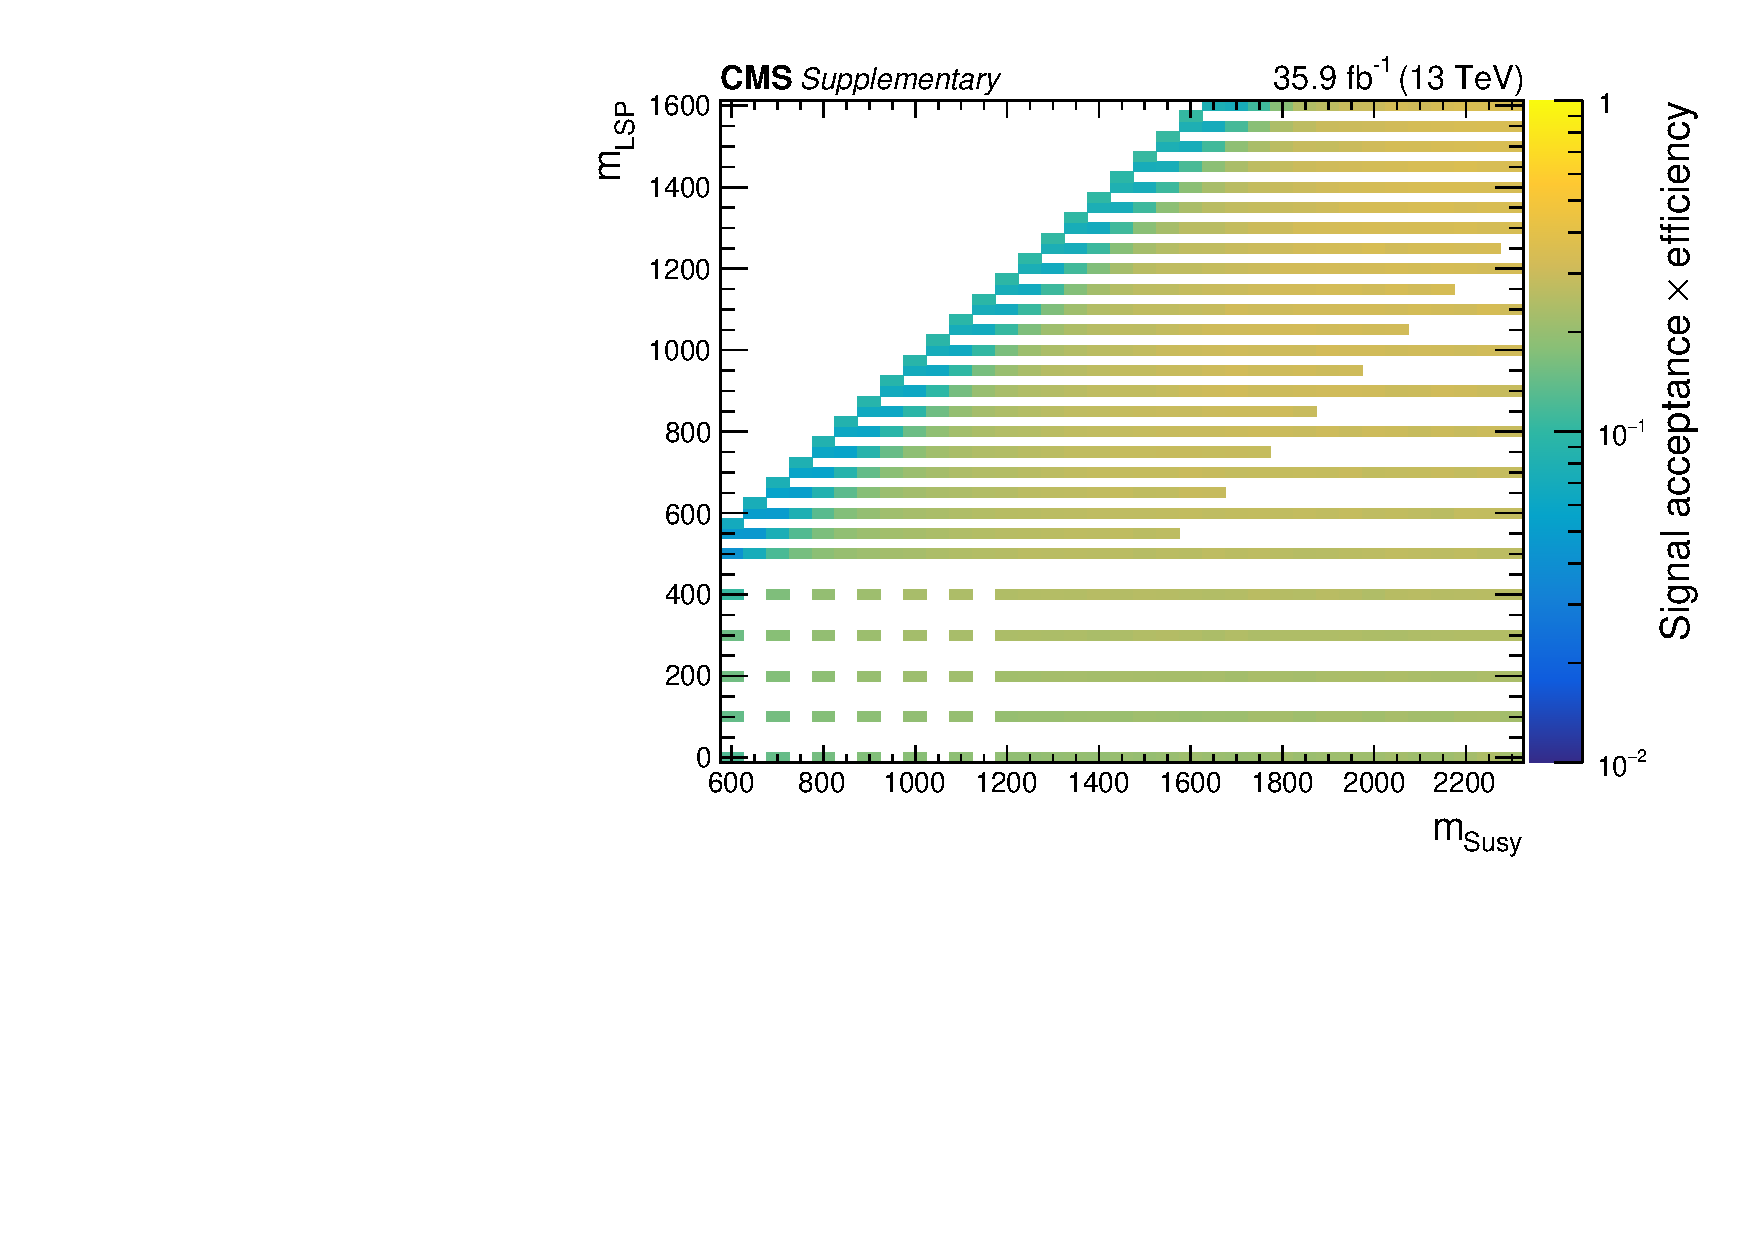
\includegraphics[width=0.45\textwidth]{figures/LLPResults/T1qqqqLL_ctau-1_effs}
            \label{fig:T1qqqqLL_eff_ctau-1}
        } ~~
        \subfigure[T1qqqqLL ($\ctau = 1\unit{mm}$): Most sensitive categories]{
            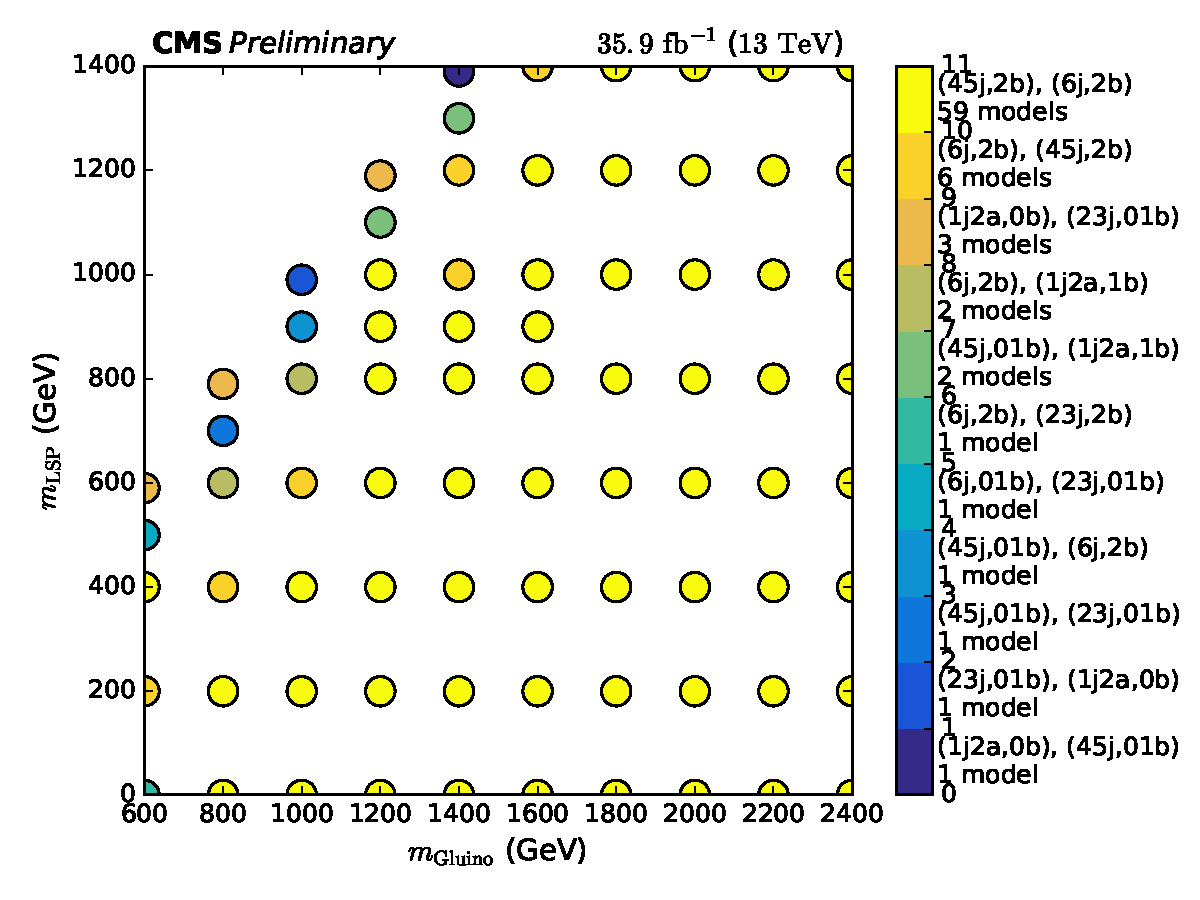
\includegraphics[width=0.45\textwidth]{figures/LLPResults/T1qqqqLL_ctau-1_bitMap}
            \label{fig:T1qqqqLL_bitMap_ctau-1}
        } \\
        %\subfigure[T1qqqqLL ($\ctau = 1\unit{mm}$): Significance scan]{
        %    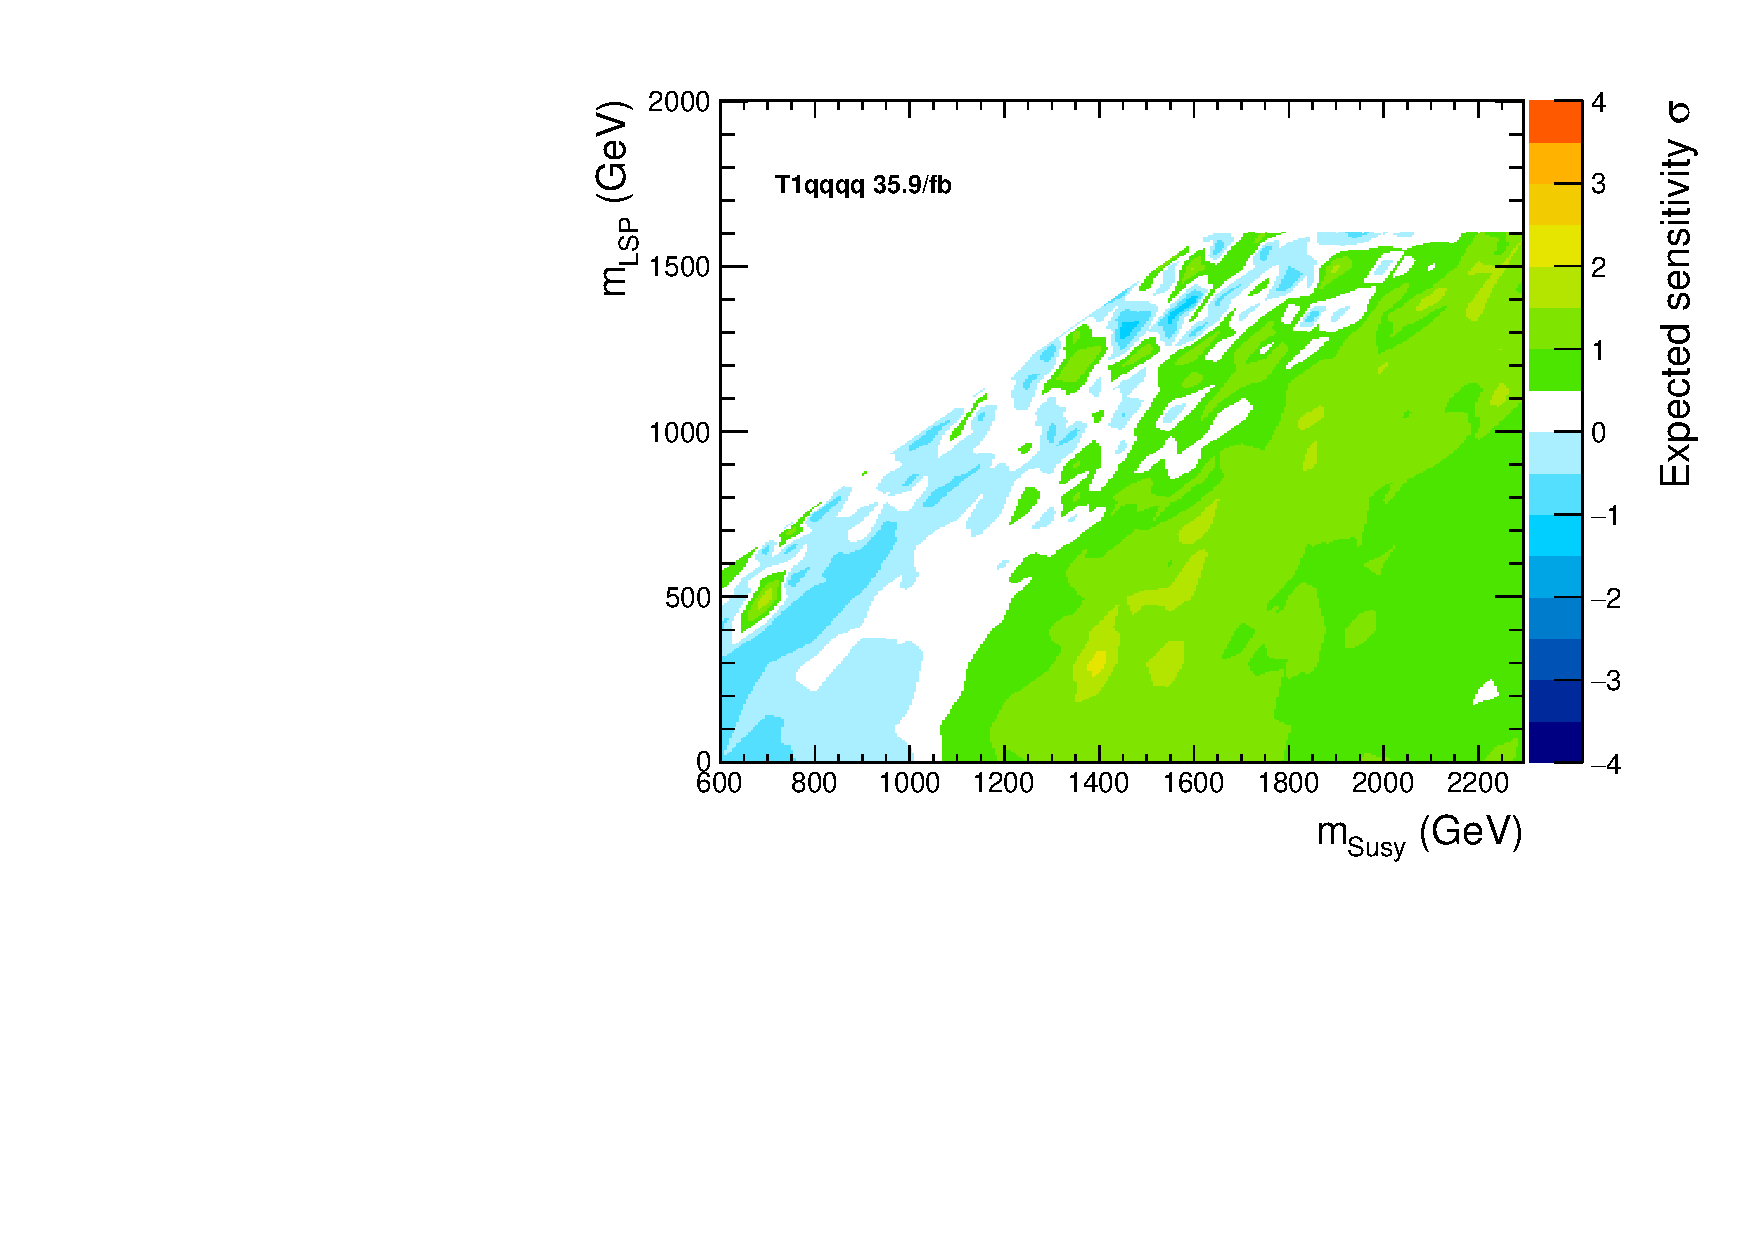
\includegraphics[width=0.45\linewidth]{figures/LLPResults/T1qqqqLL_ctau-1_signif}
        %    \label{fig:T1qqqqLL_signif_ctau-1}
        %} ~~
        \caption{Top: the 95\% C.L. observed upper limit on the cross section
            (histogram), with the expected (solid black line) observed
            (solid red line) exclusion contours. Left: signal acceptance
            including all jet categories. Right: graph showing the most 
            sensitive event topologies for each mass point.
            %Bottom: local observed significance scan.
        }
        \label{fig:T1qqqqLL:ctau-1}
    \end{center}
\end{figure}

\newpage
\begin{figure}[h!]
    \begin{center}
        \subfigure[T1qqqqLL ($\ctau = 10\unit{mm}$): Upper limit on the cross section in the mass plane]{
            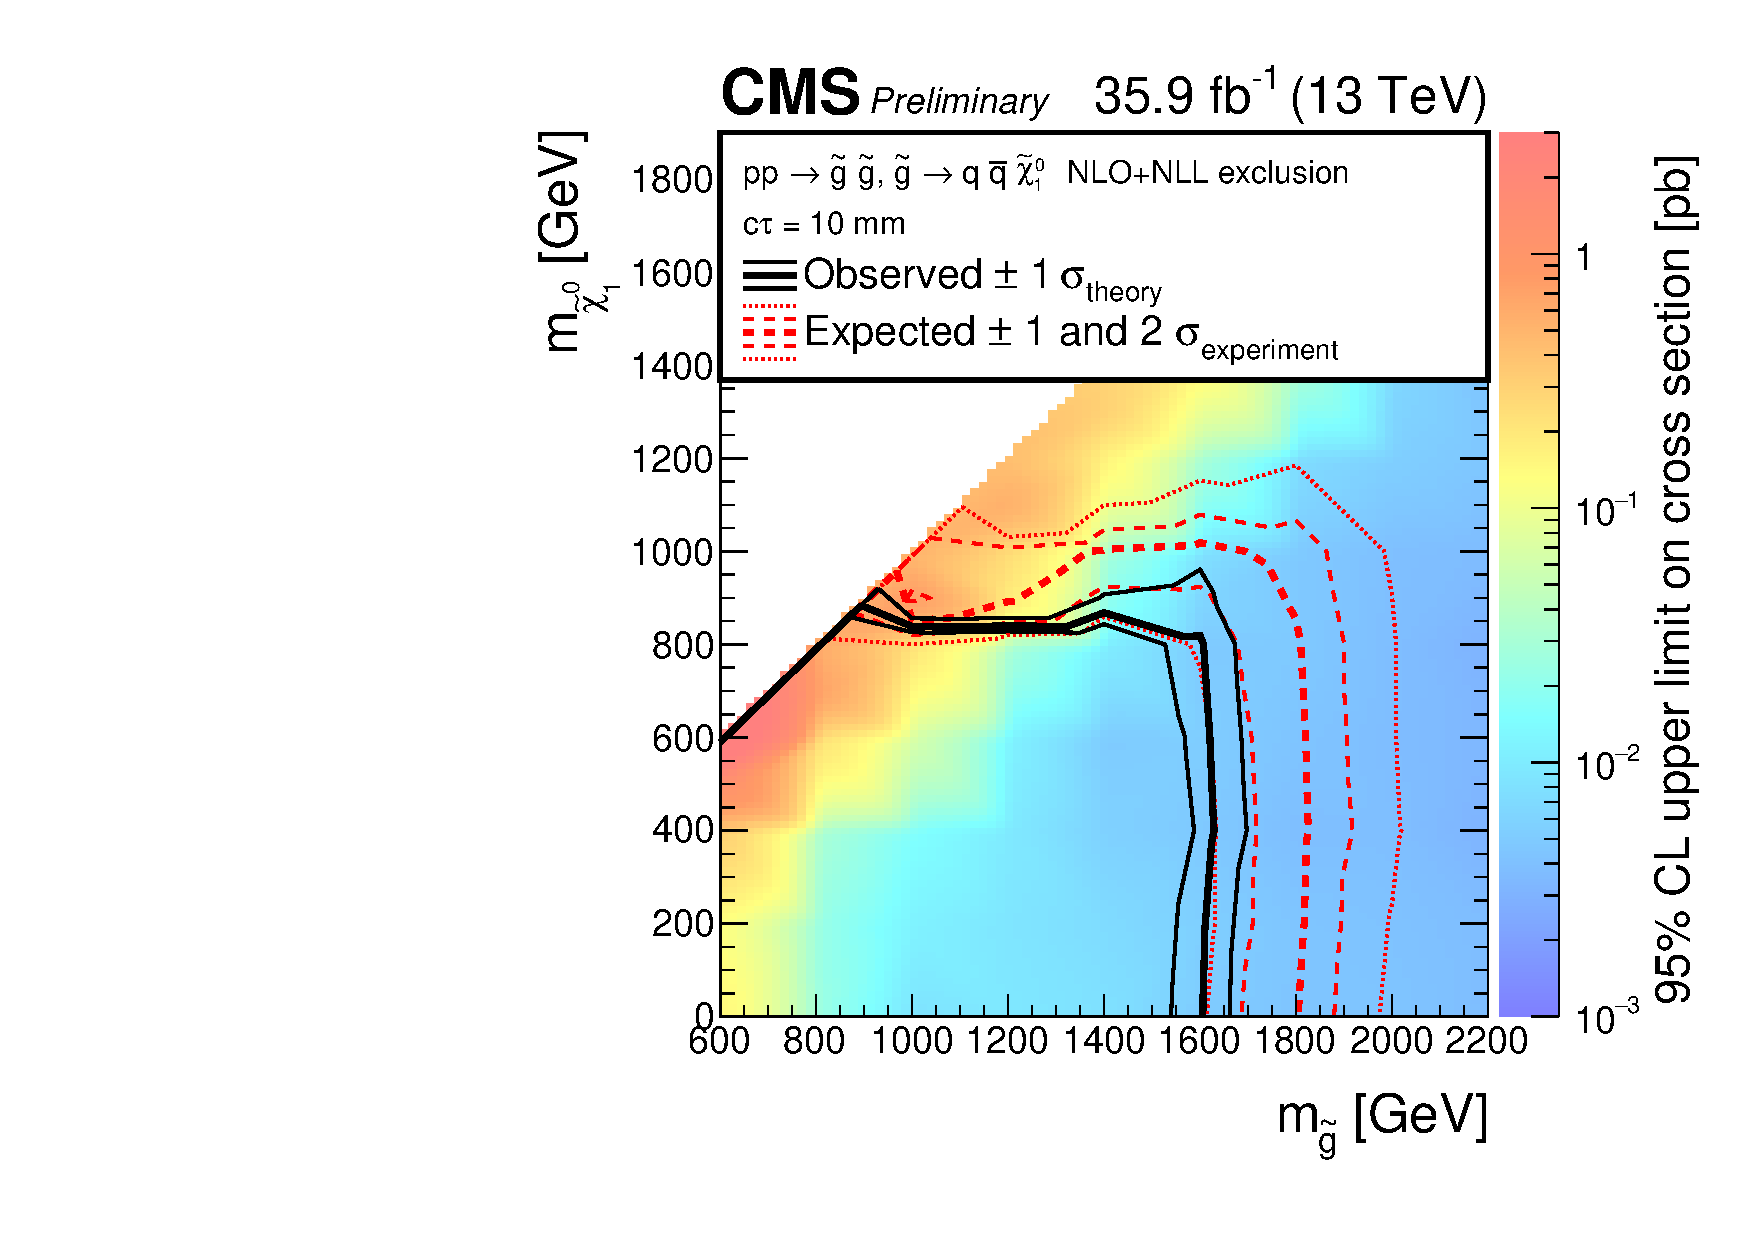
\includegraphics[width=0.6\textwidth]{figures/LLPResults/T1qqqqLL_ctau-10_XSEC}
            \label{fig:T1qqqqLL_excl_ctau-10}
        } \\
        \subfigure[T1qqqqLL ($\ctau = 10\unit{mm}$): $\epsilon_{sig}$]{
            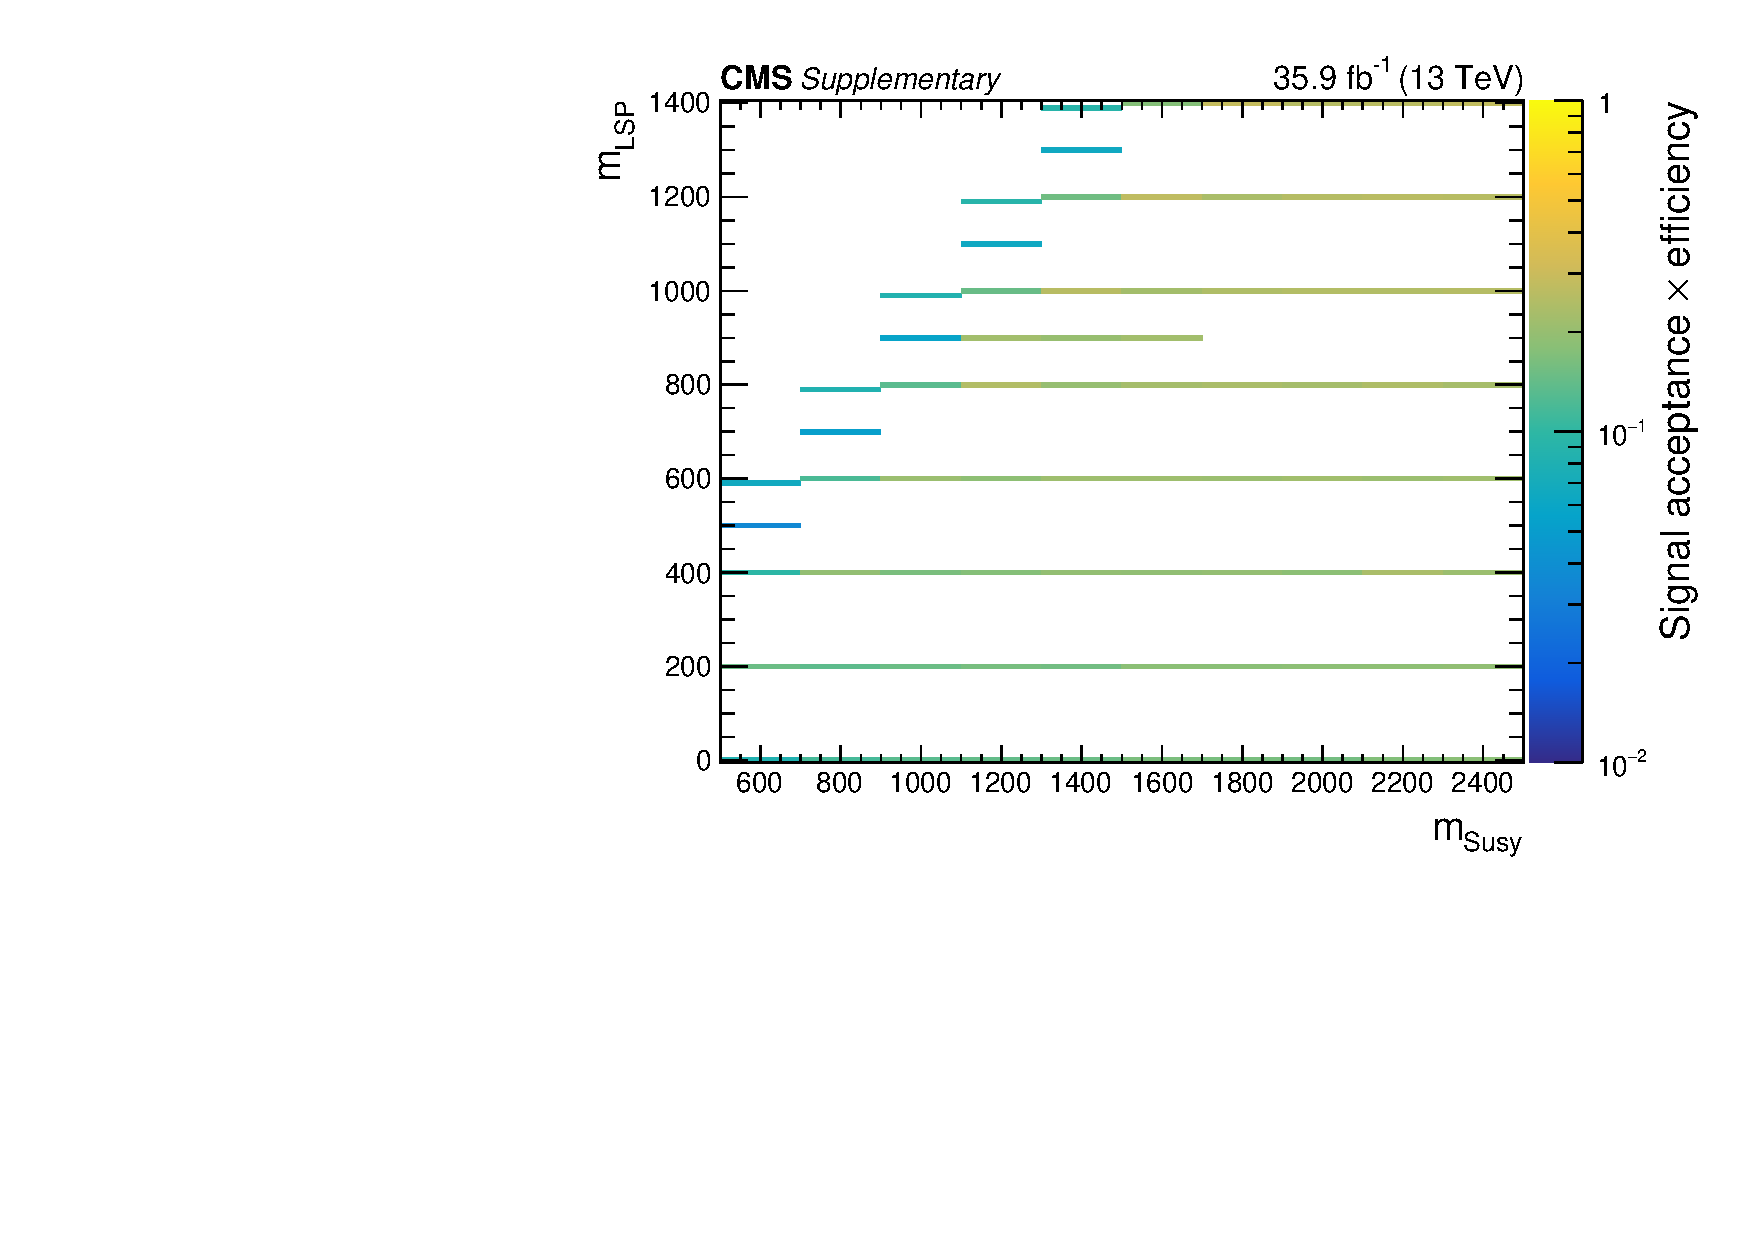
\includegraphics[width=0.45\textwidth]{figures/LLPResults/T1qqqqLL_ctau-10_effs}
            \label{fig:T1qqqqLL_eff_ctau-10}
        } ~~
        \subfigure[T1qqqqLL ($\ctau = 10\unit{mm}$): Most sensitive categories]{
            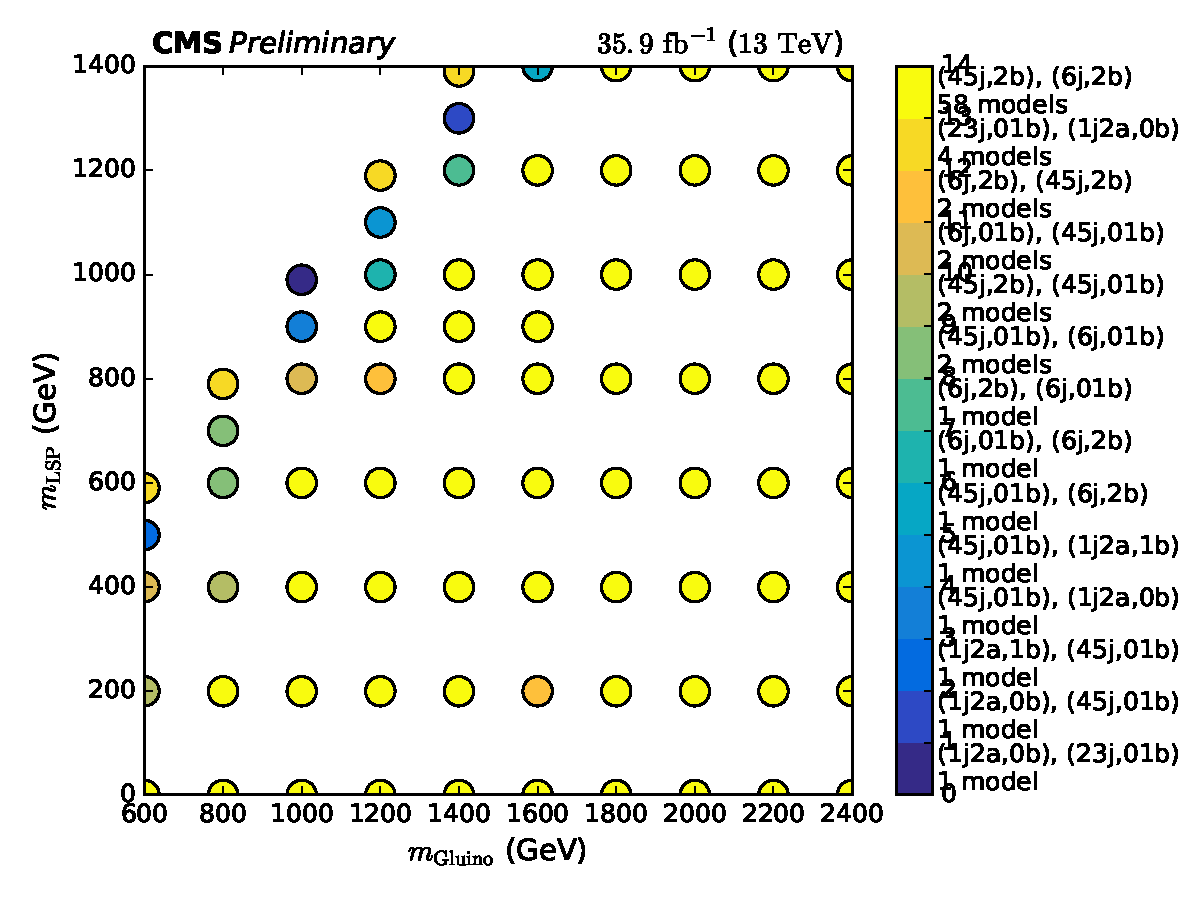
\includegraphics[width=0.45\textwidth]{figures/LLPResults/T1qqqqLL_ctau-10_bitMap}
            \label{fig:T1qqqqLL_bitMap_ctau-10}
        } \\
        %\subfigure[T1qqqqLL ($\ctau = 1\unit{mm}$): Significance scan]{
        %    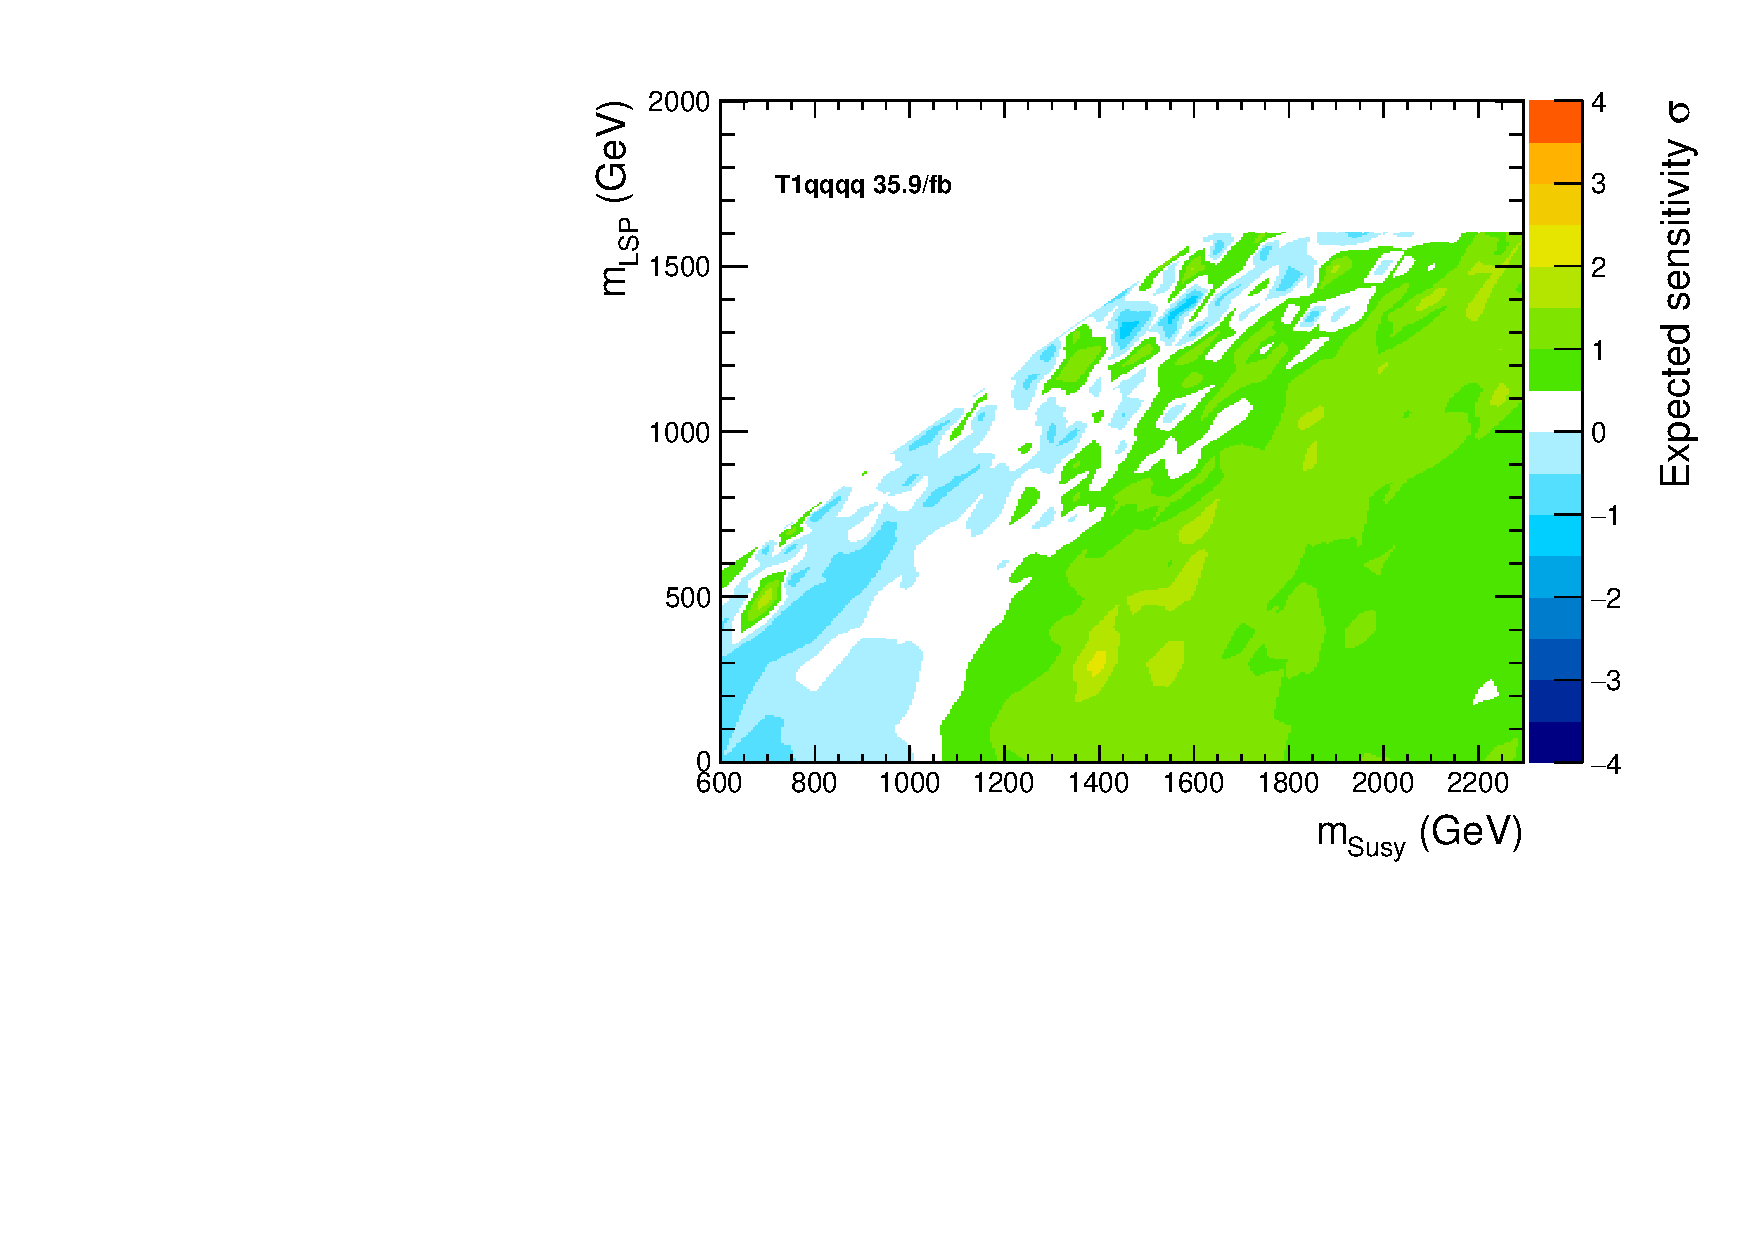
\includegraphics[width=0.45\linewidth]{figures/LLPResults/T1qqqqLL_ctau-1_signif}
        %    \label{fig:T1qqqqLL_signif_ctau-10}
        %} ~~
        \caption{Top: the 95\% C.L. observed upper limit on the cross section
            (histogram), with the expected (solid black line) observed
            (solid red line) exclusion contours. Left: signal acceptance
            including all jet categories. Right: graph showing the most 
            sensitive event topologies for each mass point.
            %Bottom: local observed significance scan.
        }
        \label{fig:T1qqqqLL:ctau-10}
    \end{center}
\end{figure}

\newpage
\begin{figure}[h!]
    \begin{center}
        \subfigure[T1qqqqLL ($\ctau = 100\unit{mm}$): Upper limit on the cross section in the mass plane]{
            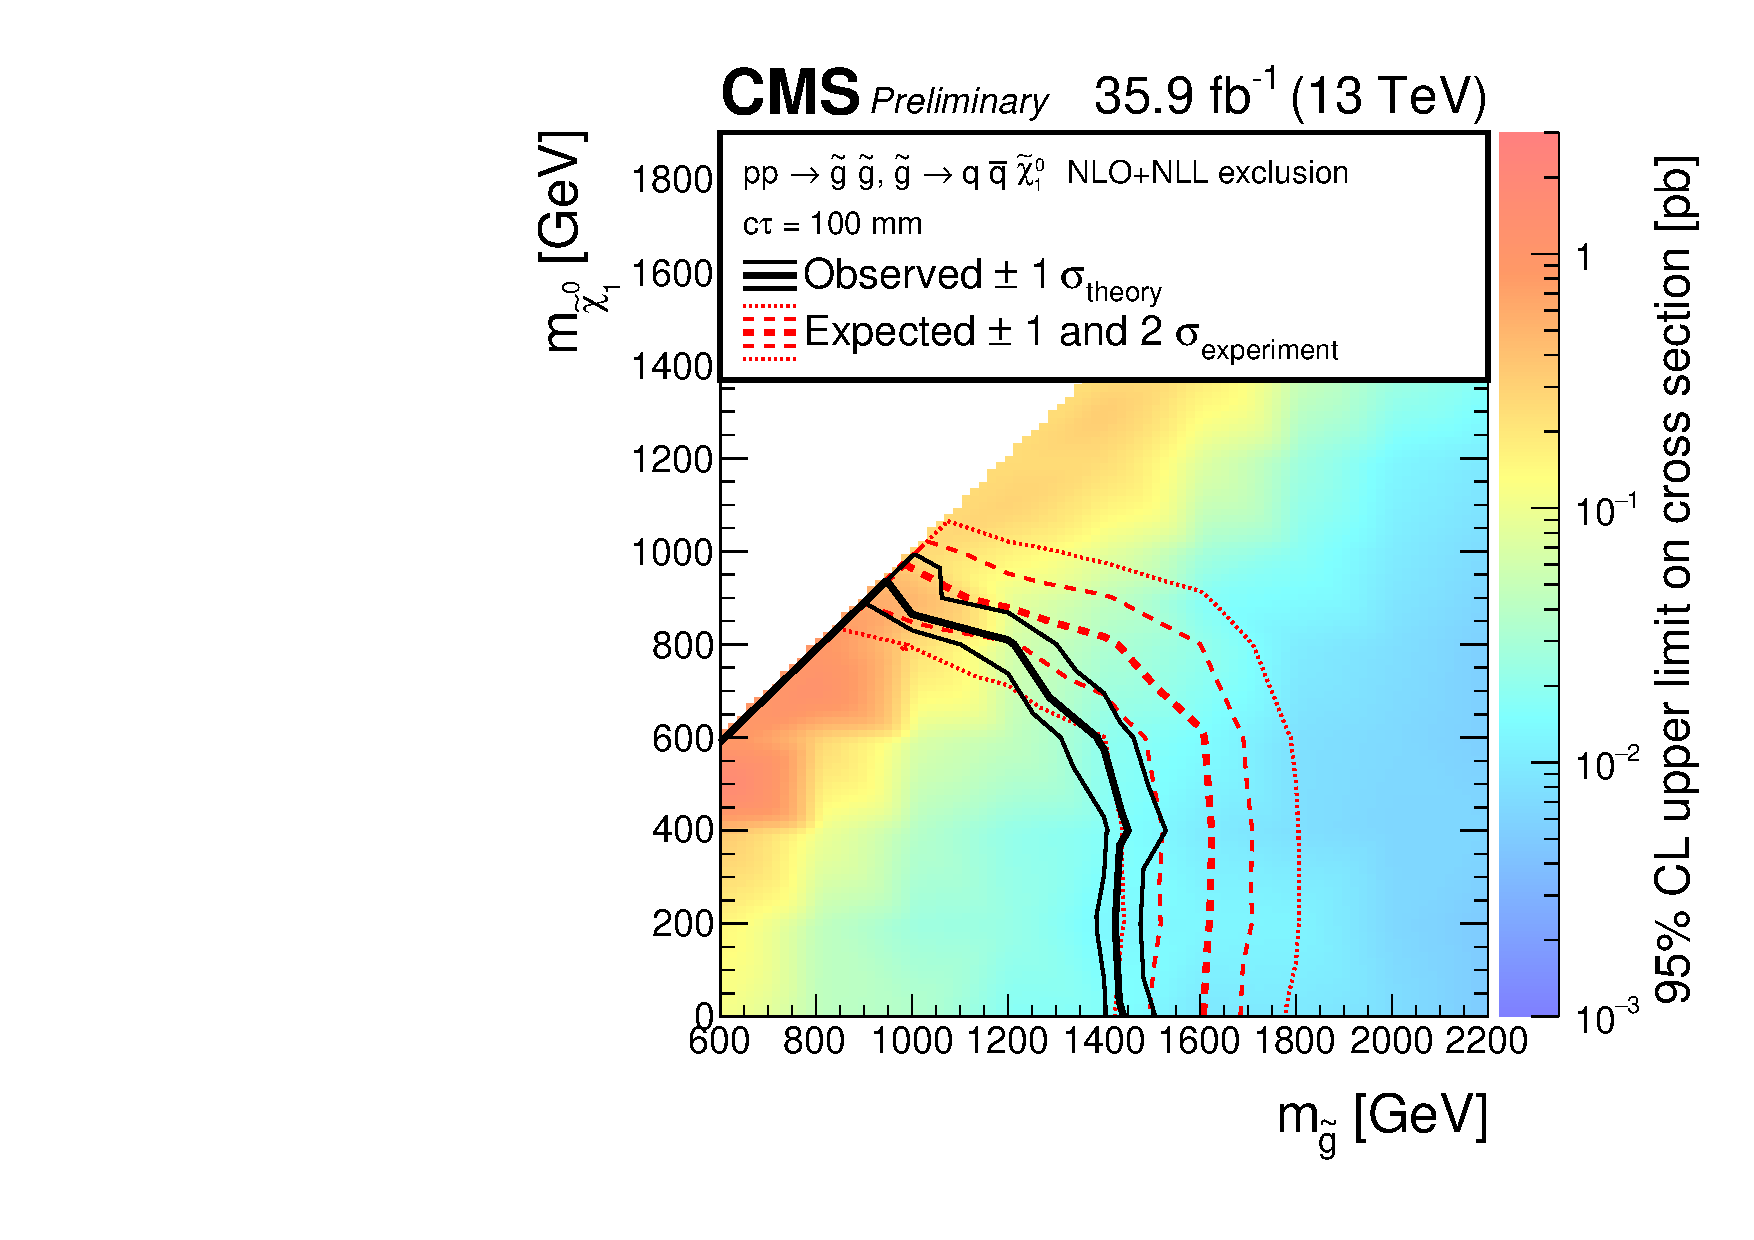
\includegraphics[width=0.6\textwidth]{figures/LLPResults/T1qqqqLL_ctau-100_XSEC}
            \label{fig:T1qqqqLL_excl_ctau-100}
        } \\
        \subfigure[T1qqqqLL ($\ctau = 100\unit{mm}$): $\epsilon_{sig}$]{
            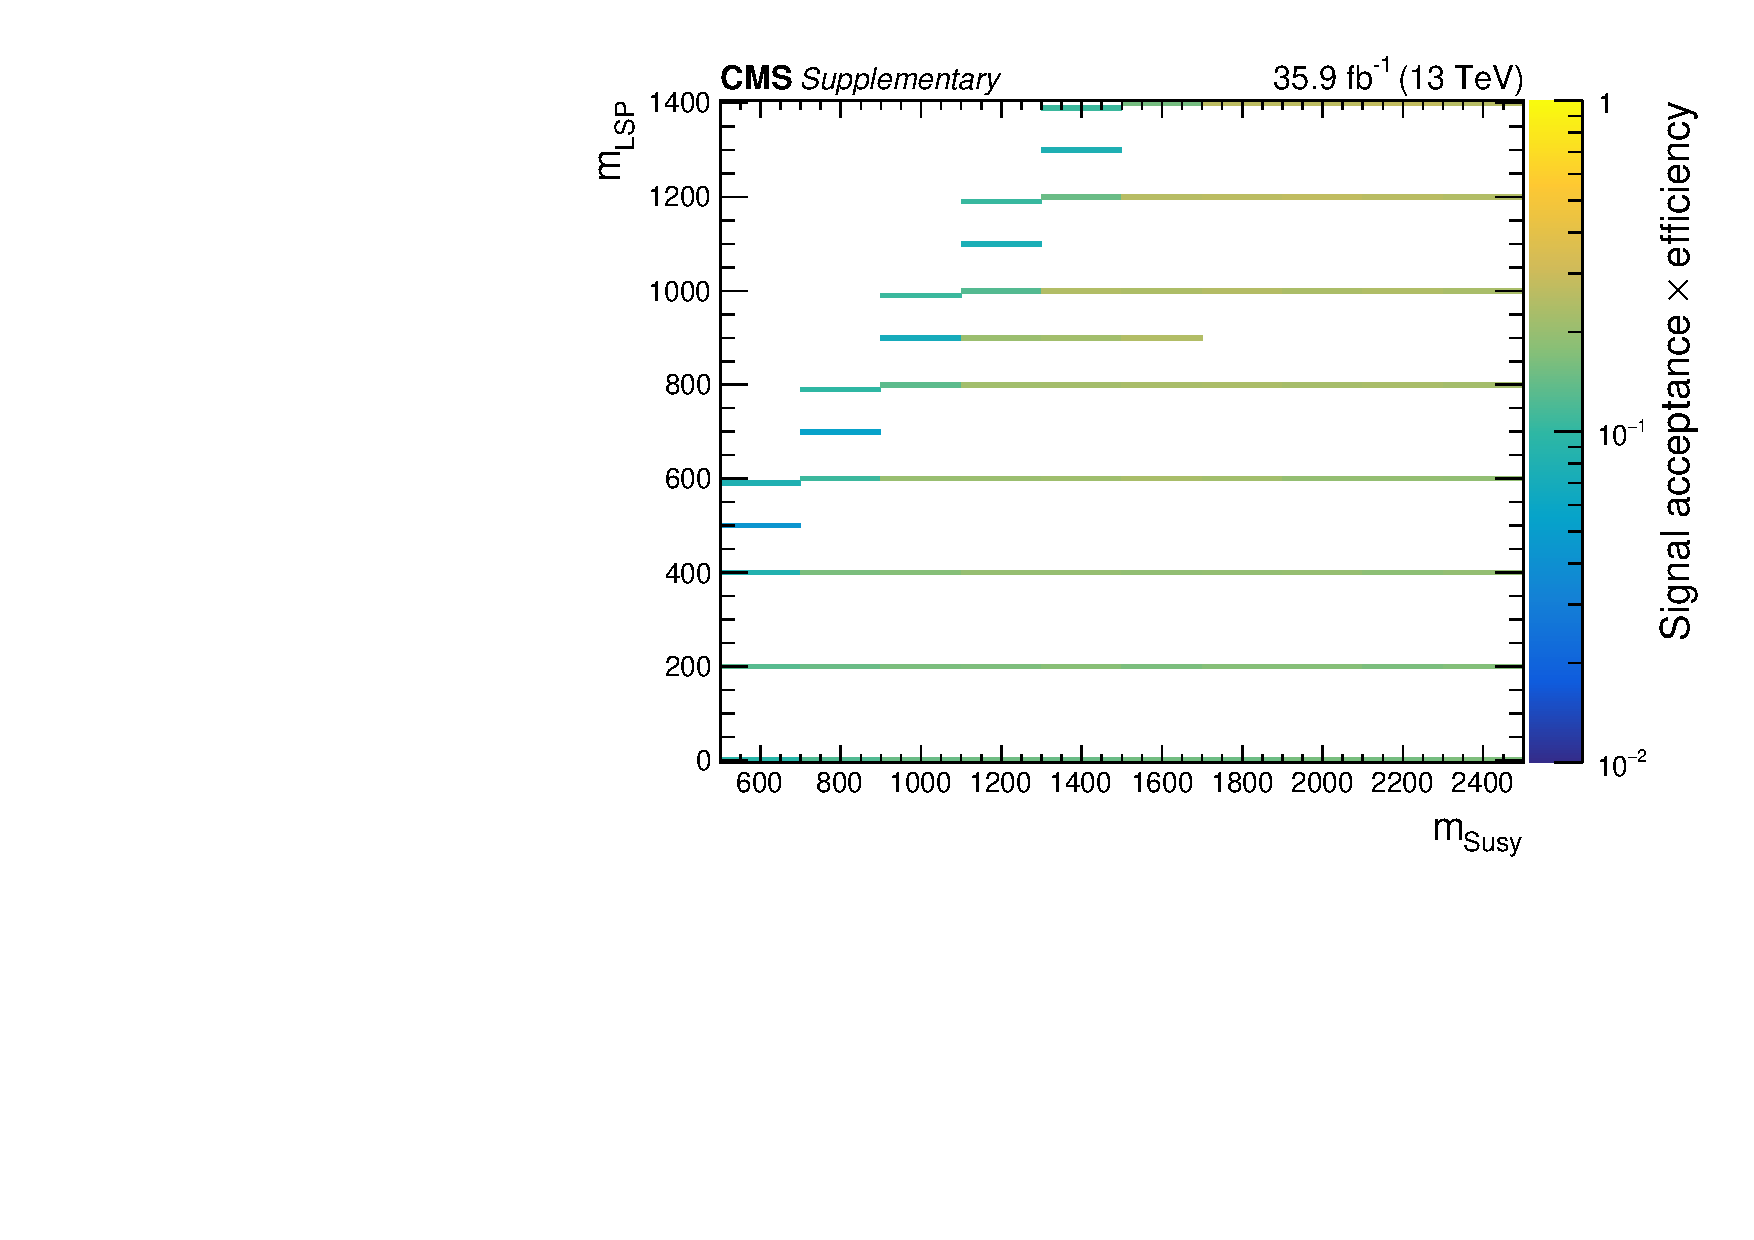
\includegraphics[width=0.45\textwidth]{figures/LLPResults/T1qqqqLL_ctau-100_effs}
            \label{fig:T1qqqqLL_eff_ctau-100}
        } ~~
        \subfigure[T1qqqqLL ($\ctau = 100\unit{mm}$): Most sensitive categories]{
            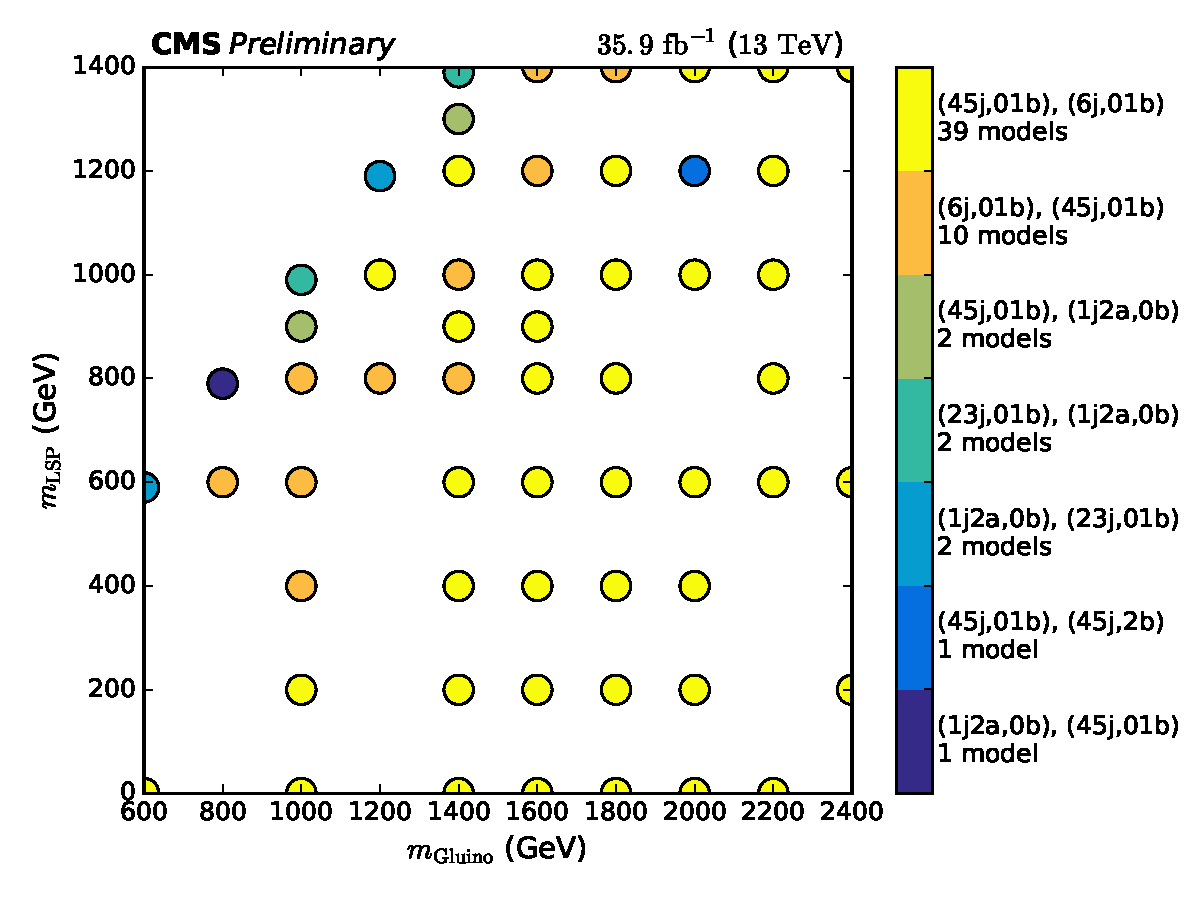
\includegraphics[width=0.45\textwidth]{figures/LLPResults/T1qqqqLL_ctau-100_bitMap}
            \label{fig:T1qqqqLL_bitMap_ctau-100}
        } \\
        %\subfigure[T1qqqqLL ($\ctau = 1\unit{mm}$): Significance scan]{
        %    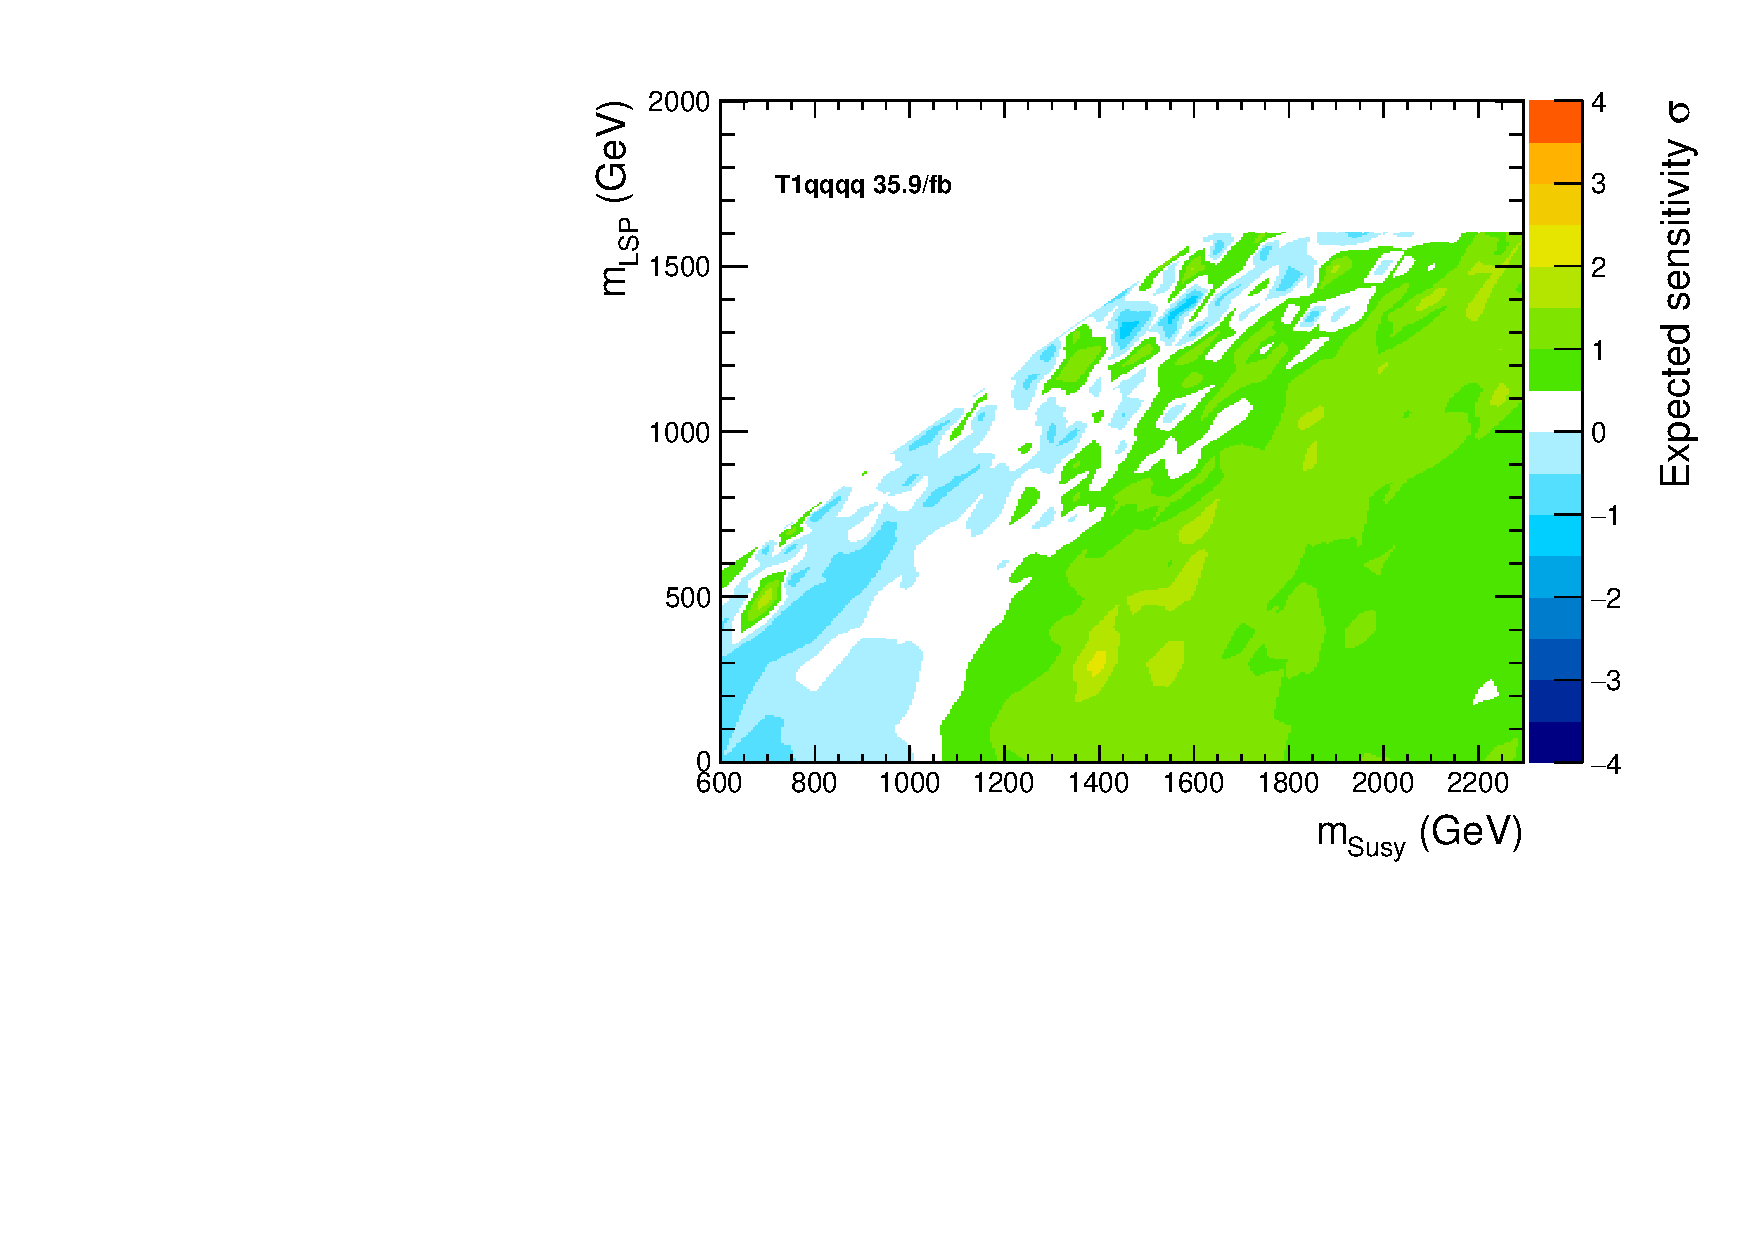
\includegraphics[width=0.45\linewidth]{figures/LLPResults/T1qqqqLL_ctau-1_signif}
        %    \label{fig:T1qqqqLL_signif_ctau-100}
        %} ~~
        \caption{Top: the 95\% C.L. observed upper limit on the cross section
            (histogram), with the expected (solid black line) observed
            (solid red line) exclusion contours. Left: signal acceptance
            including all jet categories. Right: graph showing the most 
            sensitive event topologies for each mass point.
            %Bottom: local observed significance scan.
        }
        \label{fig:T1qqqqLL:ctau-100}
    \end{center}
\end{figure}

\newpage
\begin{figure}[h!]
    \begin{center}
        \subfigure[T1qqqqLL ($\ctau = 1000\unit{mm}$): Upper limit on the cross section in the mass plane]{
            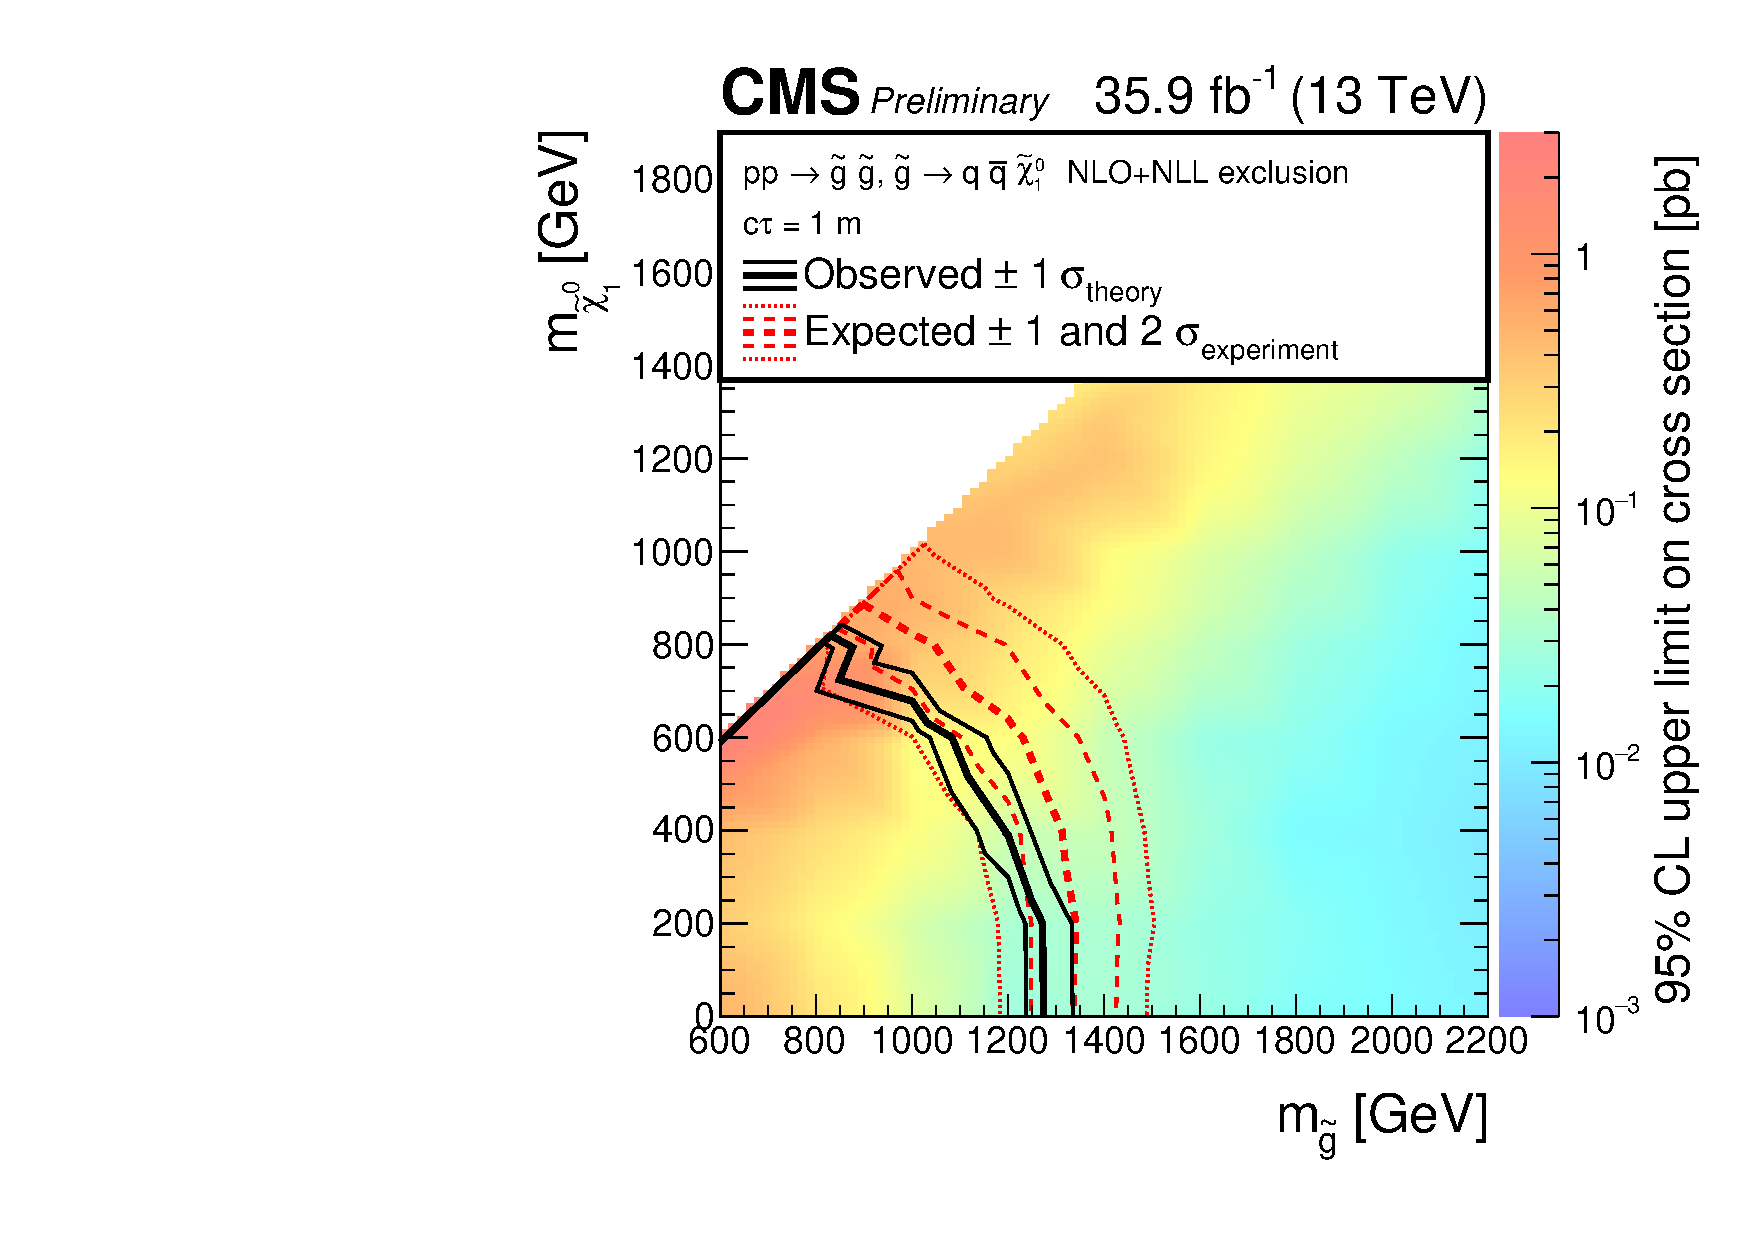
\includegraphics[width=0.6\textwidth]{figures/LLPResults/T1qqqqLL_ctau-1000_XSEC}
            \label{fig:T1qqqqLL_excl_ctau-1000}
        } \\
        \subfigure[T1qqqqLL ($\ctau = 1000\unit{mm}$): $\epsilon_{sig}$]{
            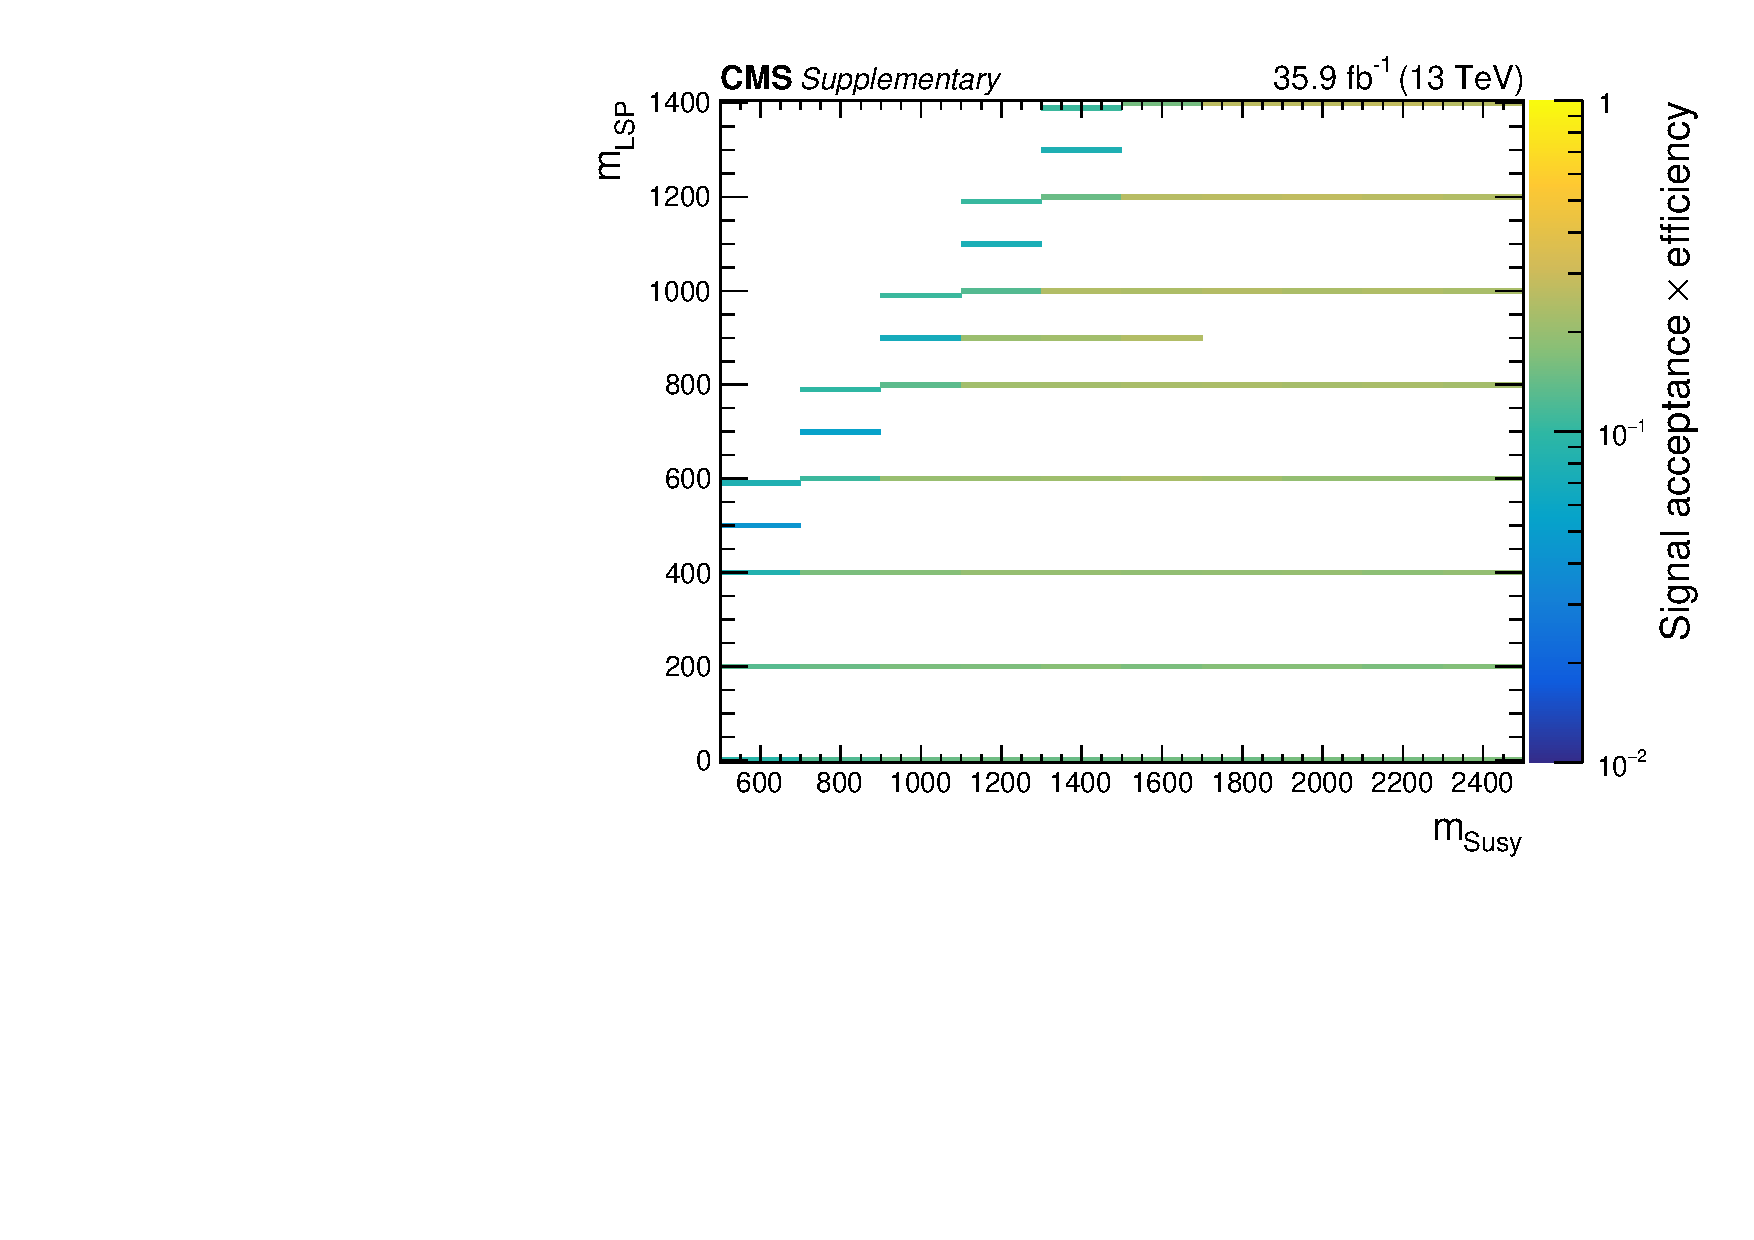
\includegraphics[width=0.45\textwidth]{figures/LLPResults/T1qqqqLL_ctau-1000_effs}
            \label{fig:T1qqqqLL_eff_ctau-1000}
        } ~~
        \subfigure[T1qqqqLL ($\ctau = 1000\unit{mm}$): Most sensitive categories]{
            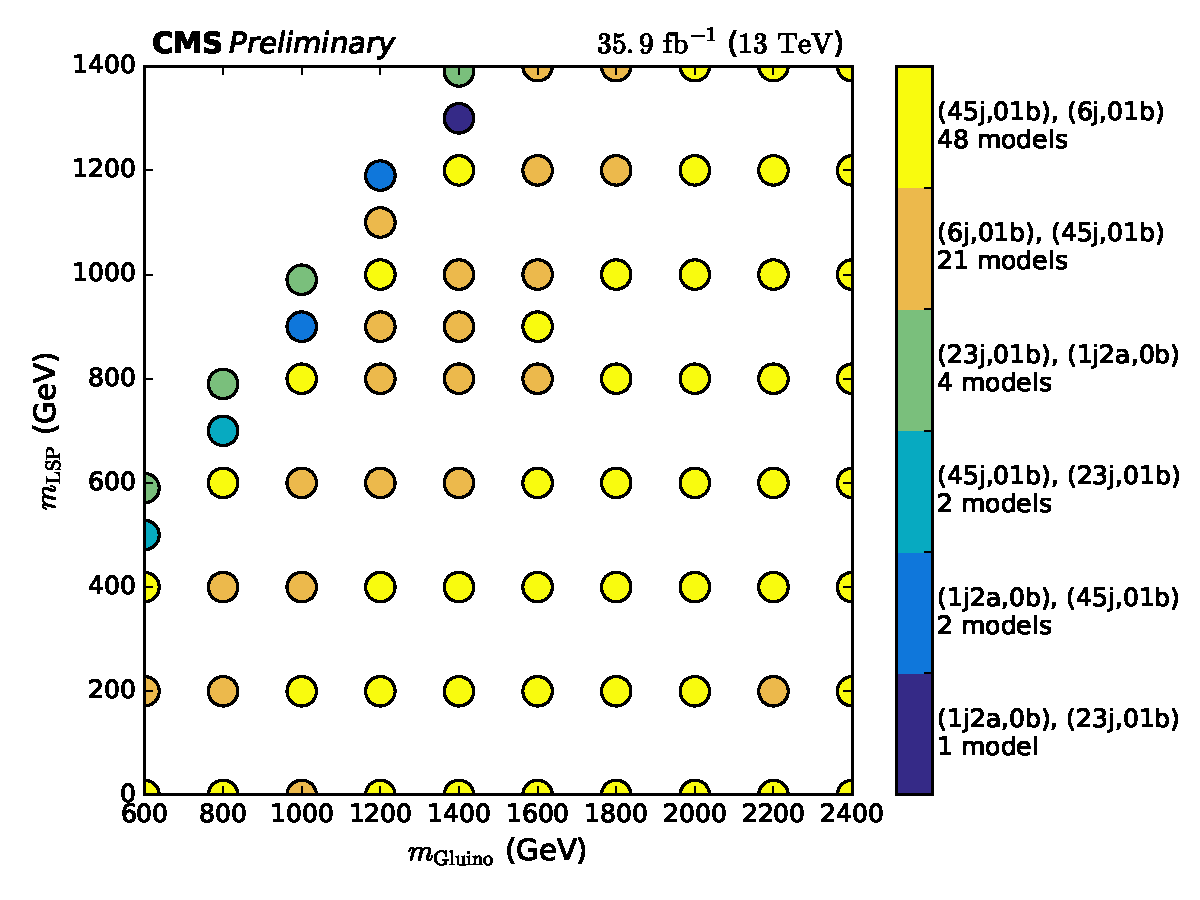
\includegraphics[width=0.45\textwidth]{figures/LLPResults/T1qqqqLL_ctau-1000_bitMap}
            \label{fig:T1qqqqLL_bitMap_ctau-1000}
        } \\
        %\subfigure[T1qqqqLL ($\ctau = 1\unit{mm}$): Significance scan]{
        %    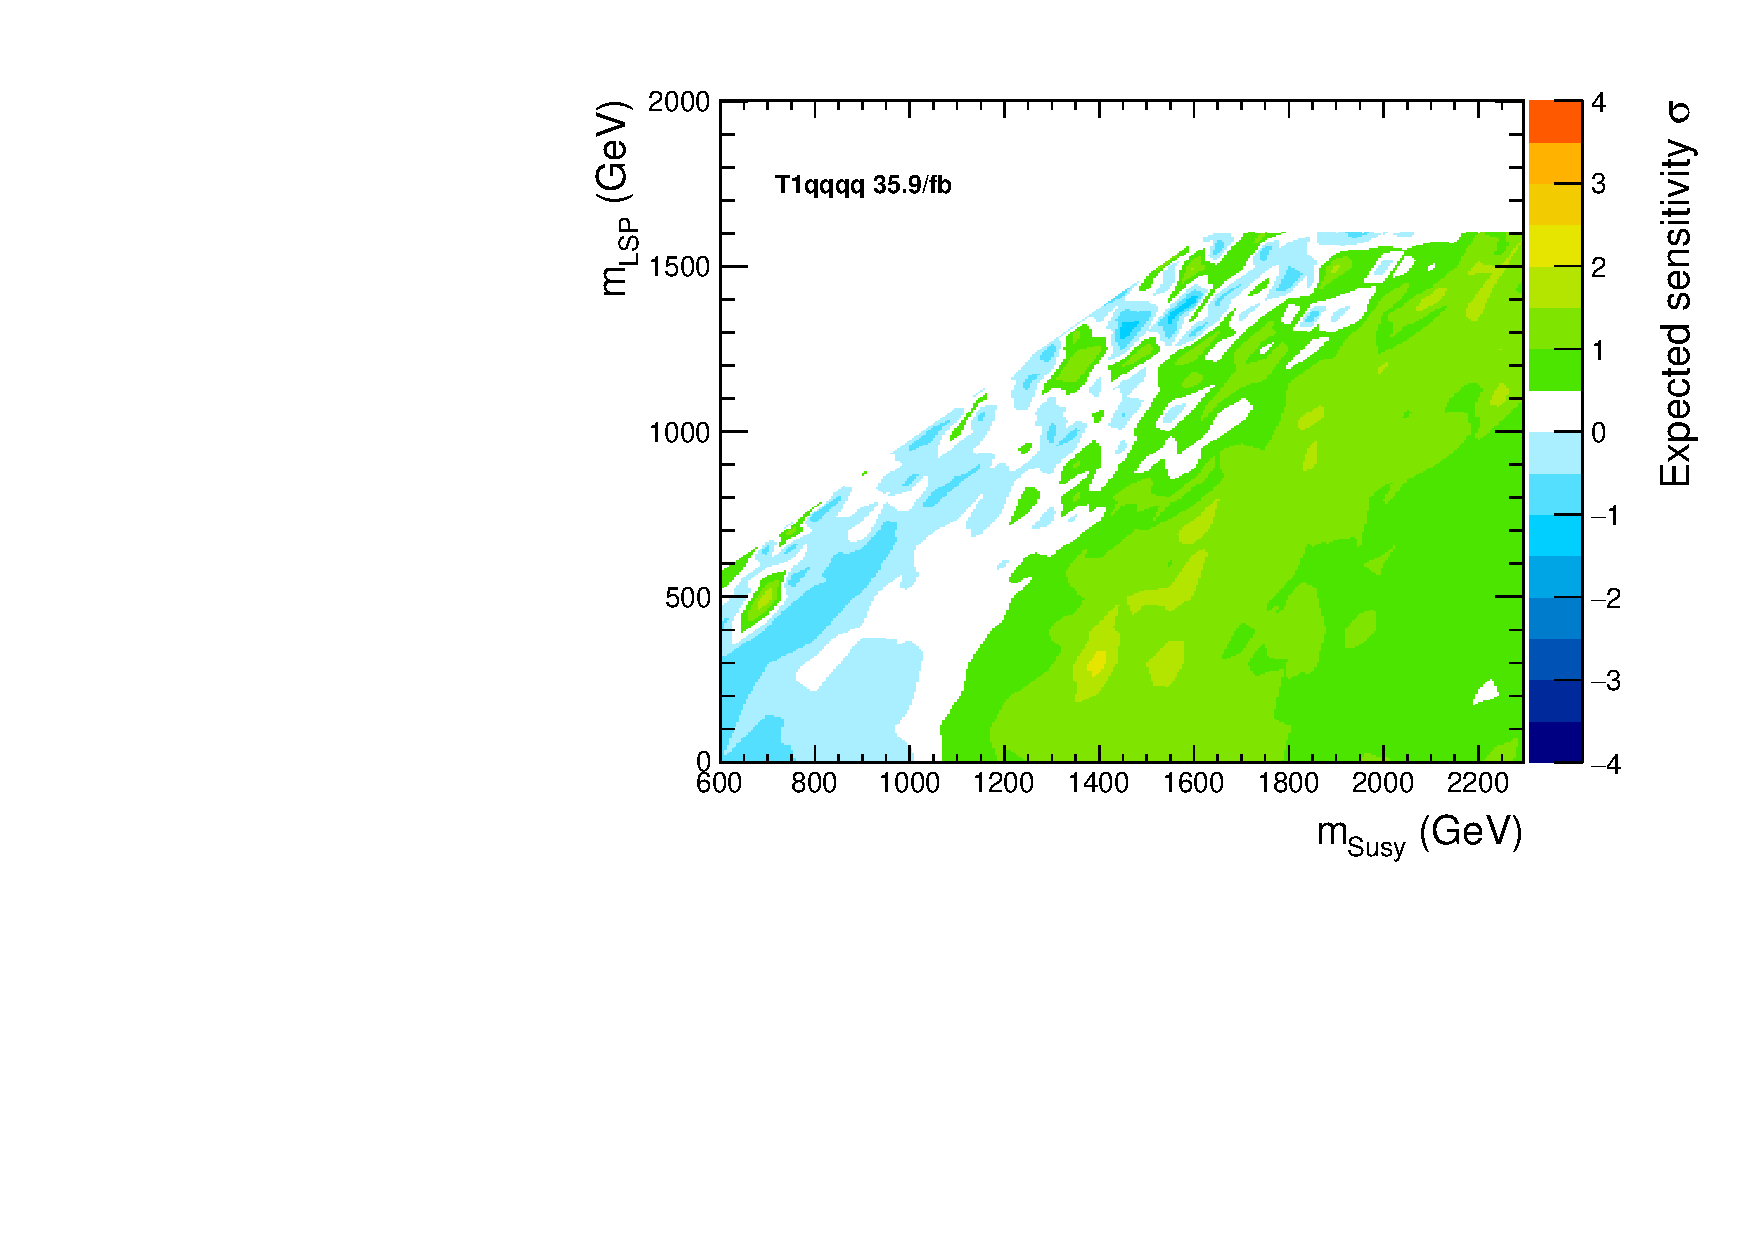
\includegraphics[width=0.45\linewidth]{figures/LLPResults/T1qqqqLL_ctau-1_signif}
        %    \label{fig:T1qqqqLL_signif_ctau-1000}
        %} ~~
        \caption{Top: the 95\% C.L. observed upper limit on the cross section
            (histogram), with the expected (solid black line) observed
            (solid red line) exclusion contours. Left: signal acceptance
            including all jet categories. Right: graph showing the most 
            sensitive event topologies for each mass point.
            %Bottom: local observed significance scan.
        }
        \label{fig:T1qqqqLL:ctau-1000}
    \end{center}
\end{figure}

\newpage
\begin{figure}[h!]
    \begin{center}
        \subfigure[T1qqqqLL ($\ctau = 10000\unit{mm}$): Upper limit on the cross section in the mass plane]{
            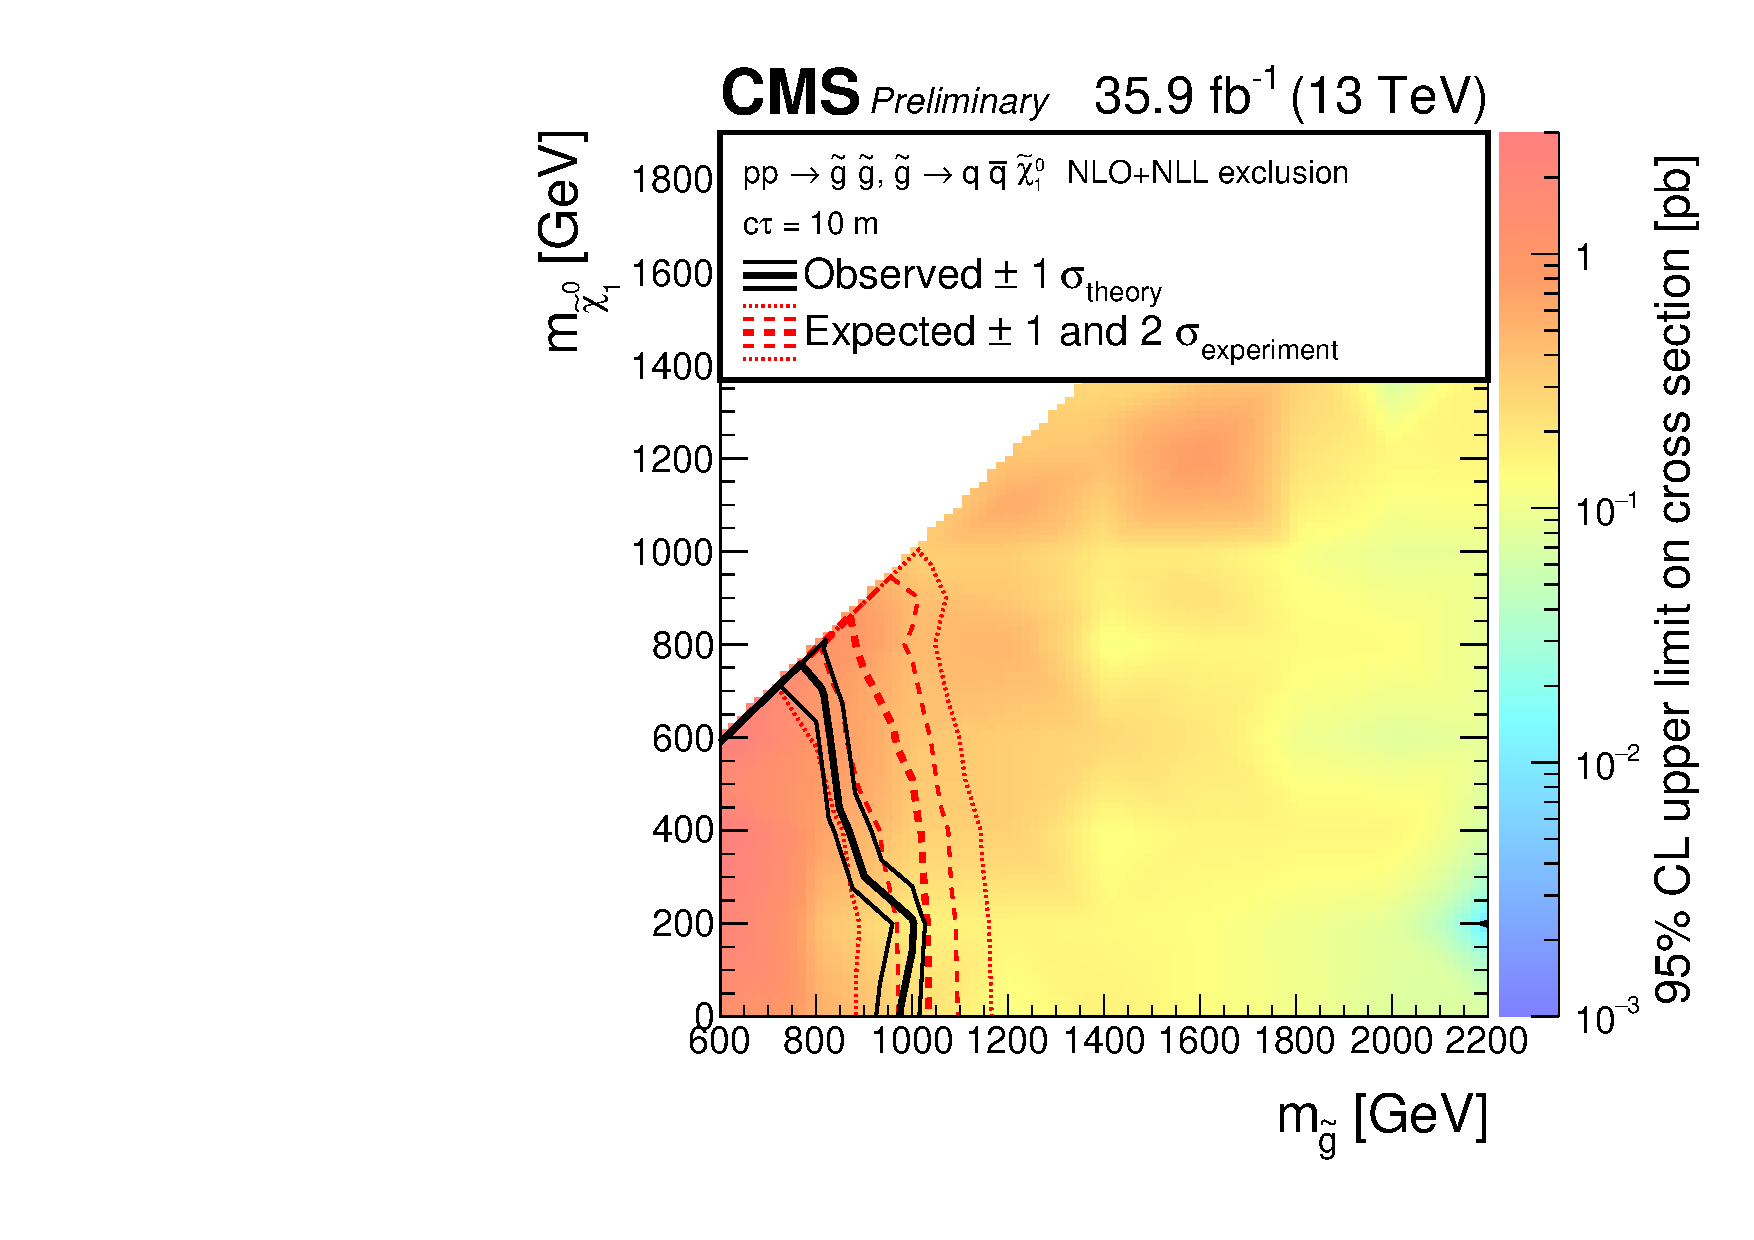
\includegraphics[width=0.6\textwidth]{figures/LLPResults/T1qqqqLL_ctau-10000_XSEC}
            \label{fig:T1qqqqLL_excl_ctau-10000}
        } \\
        \subfigure[T1qqqqLL ($\ctau = 10000\unit{mm}$): $\epsilon_{sig}$]{
            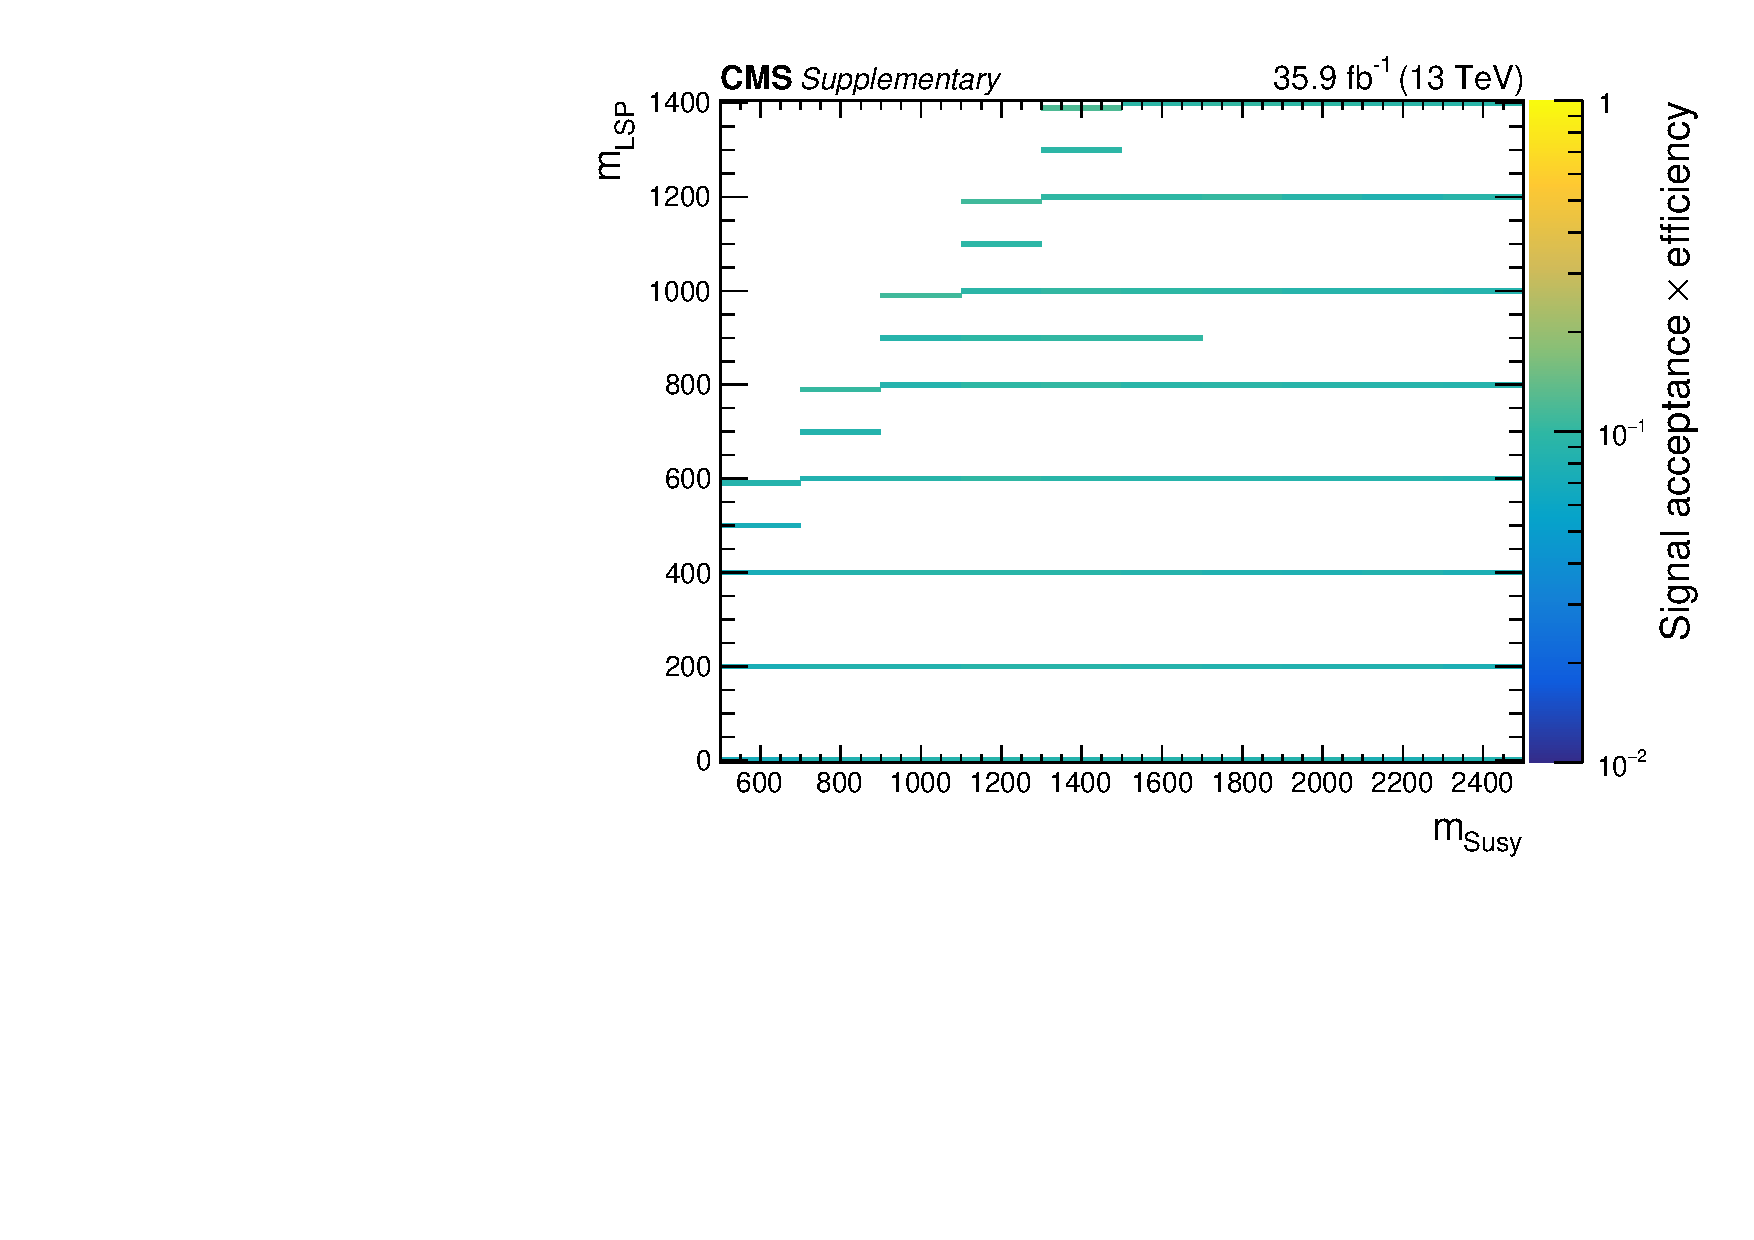
\includegraphics[width=0.45\textwidth]{figures/LLPResults/T1qqqqLL_ctau-10000_effs}
            \label{fig:T1qqqqLL_eff_ctau-10000}
        } ~~
        \subfigure[T1qqqqLL ($\ctau = 10000\unit{mm}$): Most sensitive categories]{
            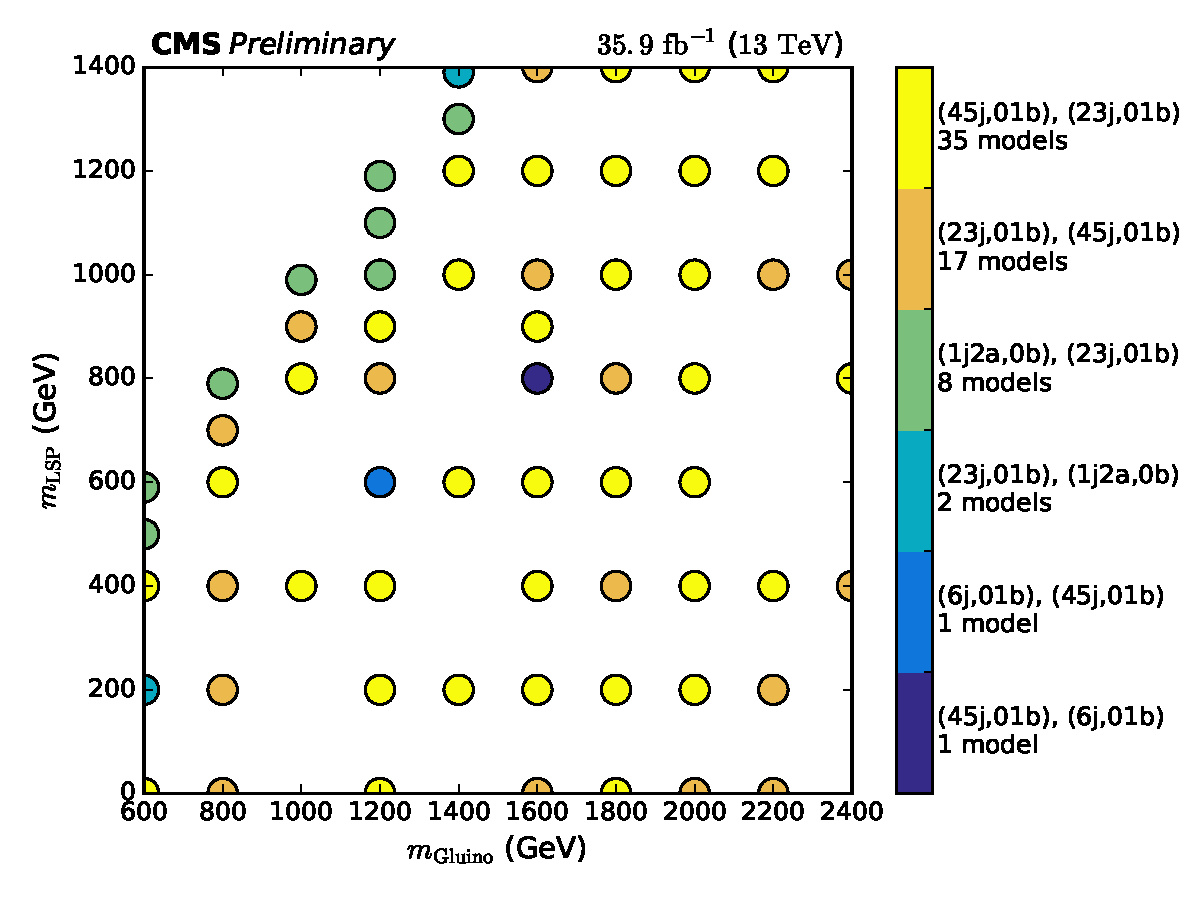
\includegraphics[width=0.45\textwidth]{figures/LLPResults/T1qqqqLL_ctau-10000_bitMap}
            \label{fig:T1qqqqLL_bitMap_ctau-10000}
        } \\
        %\subfigure[T1qqqqLL ($\ctau = 1\unit{mm}$): Significance scan]{
        %    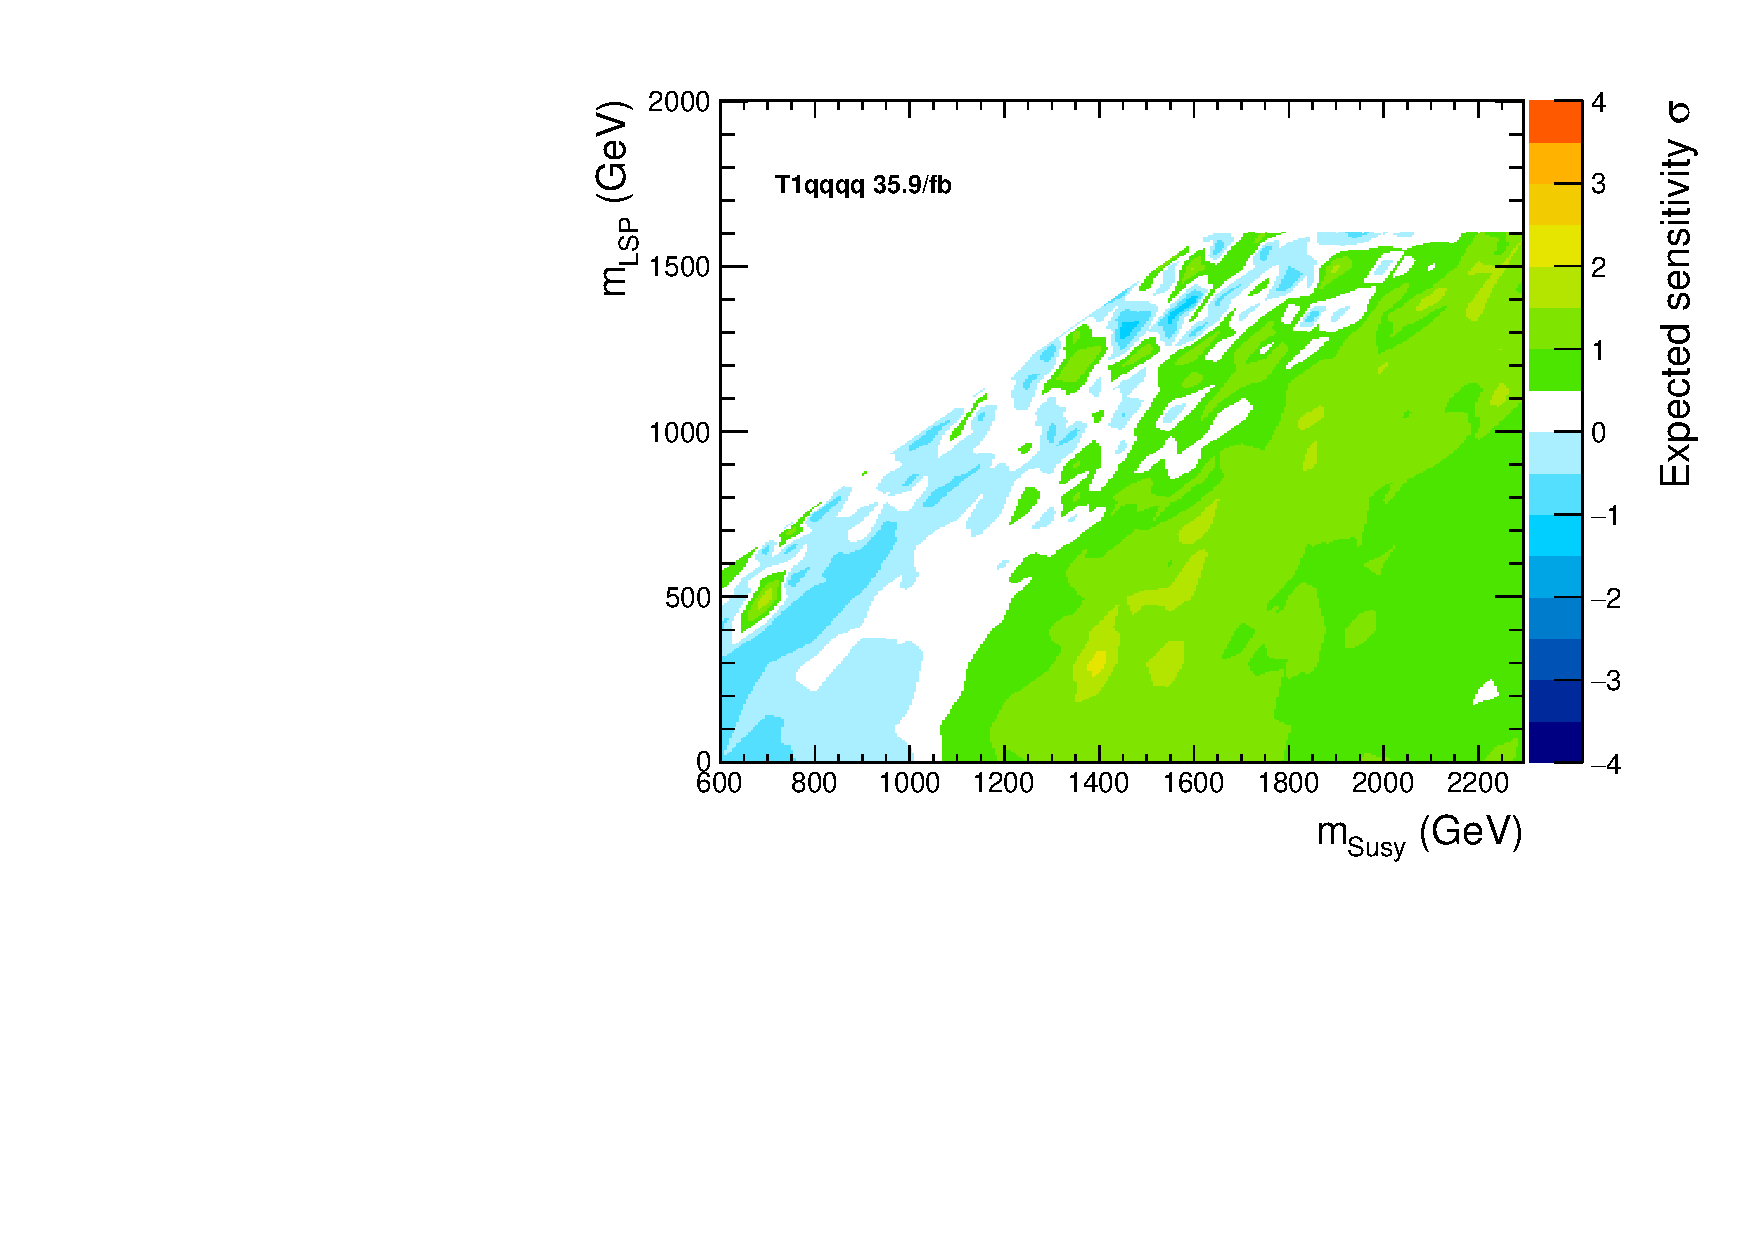
\includegraphics[width=0.45\linewidth]{figures/LLPResults/T1qqqqLL_ctau-1_signif}
        %    \label{fig:T1qqqqLL_signif_ctau-10000}
        %} ~~
        \caption{Top: the 95\% C.L. observed upper limit on the cross section
            (histogram), with the expected (solid black line) observed
            (solid red line) exclusion contours. Left: signal acceptance
            including all jet categories. Right: graph showing the most 
            sensitive event topologies for each mass point.
            %Bottom: local observed significance scan.
        }
        \label{fig:T1qqqqLL:ctau-10000}
    \end{center}
\end{figure}

\newpage
\begin{figure}[h!]
    \begin{center}
        \subfigure[T1qqqqLL ($\ctau = 100000\unit{mm}$): Upper limit on the cross section in the mass plane]{
            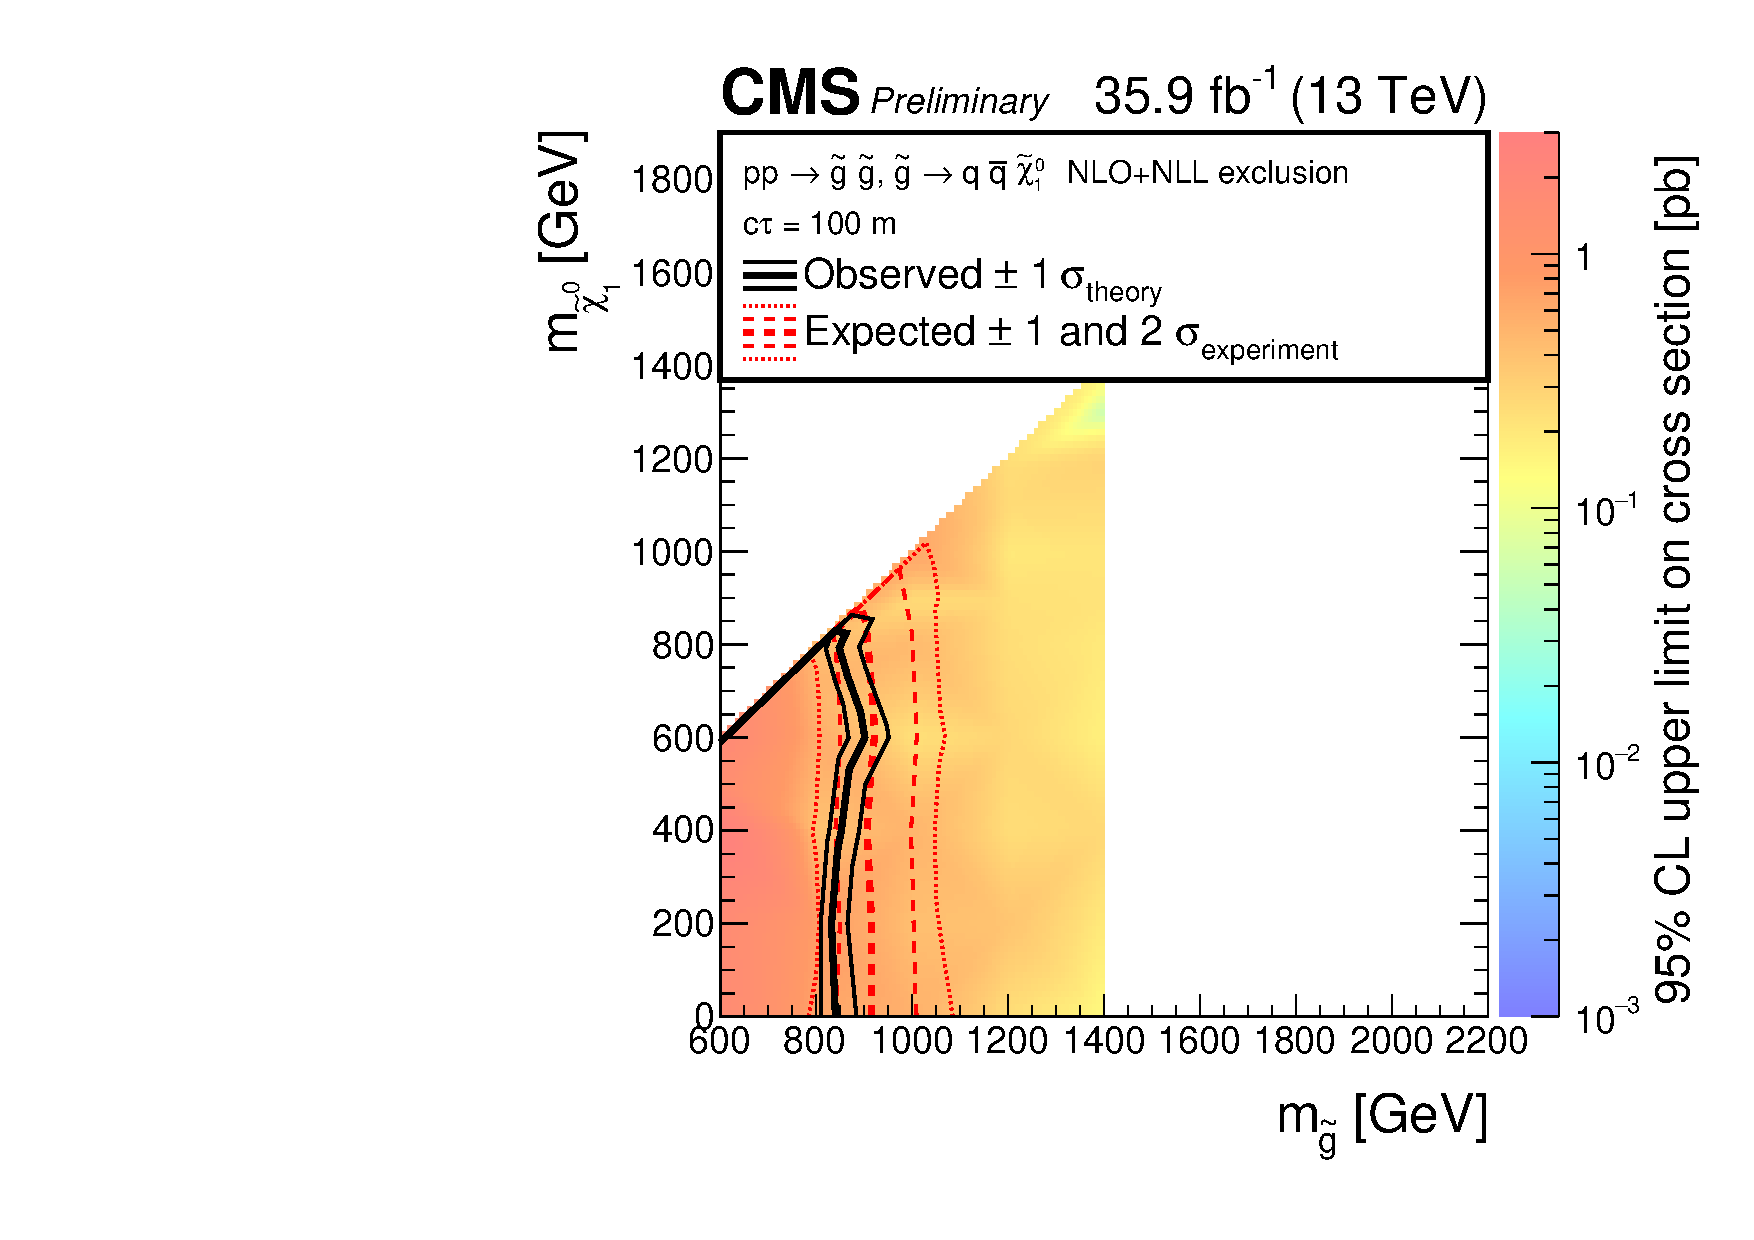
\includegraphics[width=0.6\textwidth]{figures/LLPResults/T1qqqqLL_ctau-100000_XSEC}
            \label{fig:T1qqqqLL_excl_ctau-100000}
        } \\
        \subfigure[T1qqqqLL ($\ctau = 100000\unit{mm}$): $\epsilon_{sig}$]{
            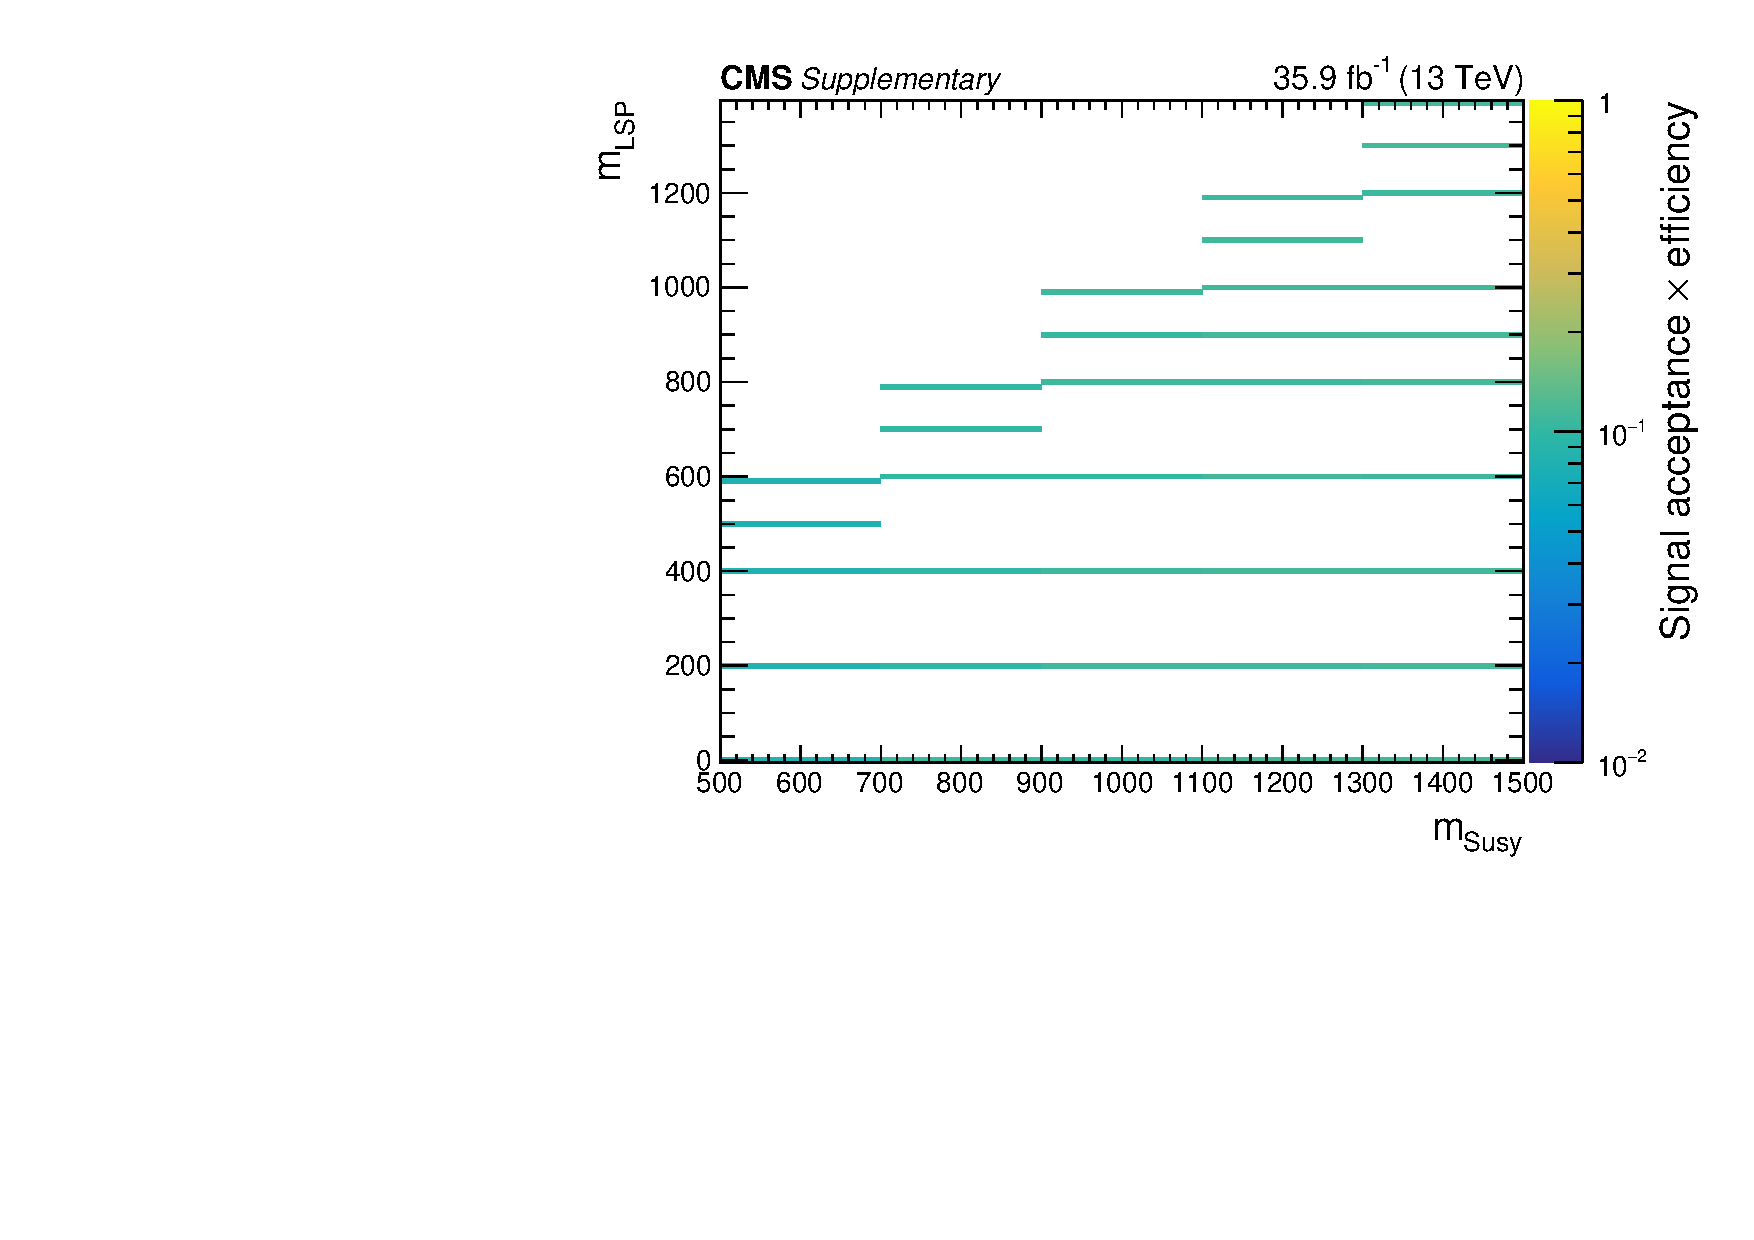
\includegraphics[width=0.45\textwidth]{figures/LLPResults/T1qqqqLL_ctau-100000_effs}
            \label{fig:T1qqqqLL_eff_ctau-100000}
        } ~~
        \subfigure[T1qqqqLL ($\ctau = 100000\unit{mm}$): Most sensitive categories]{
            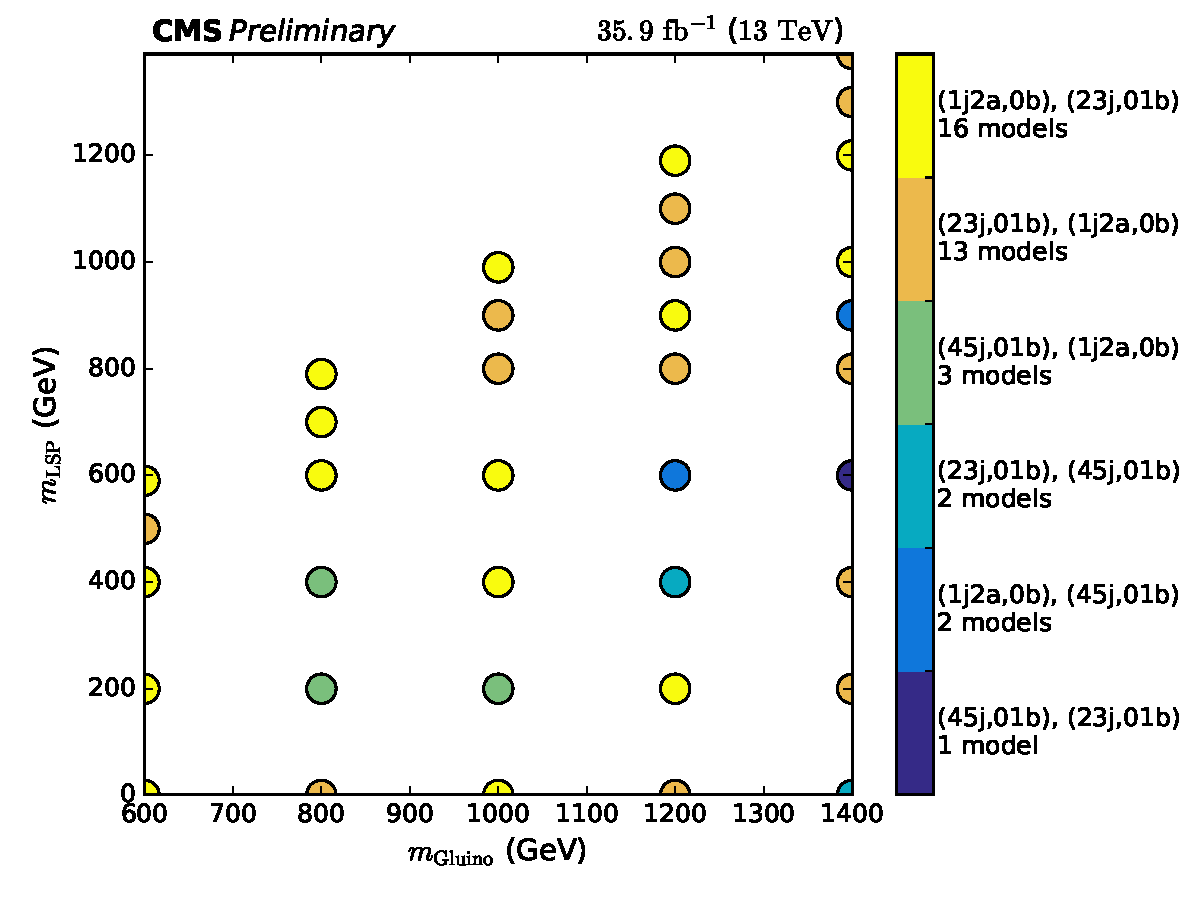
\includegraphics[width=0.45\textwidth]{figures/LLPResults/T1qqqqLL_ctau-100000_bitMap}
            \label{fig:T1qqqqLL_bitMap_ctau-100000}
        } \\
        %\subfigure[T1qqqqLL ($\ctau = 1\unit{mm}$): Significance scan]{
        %    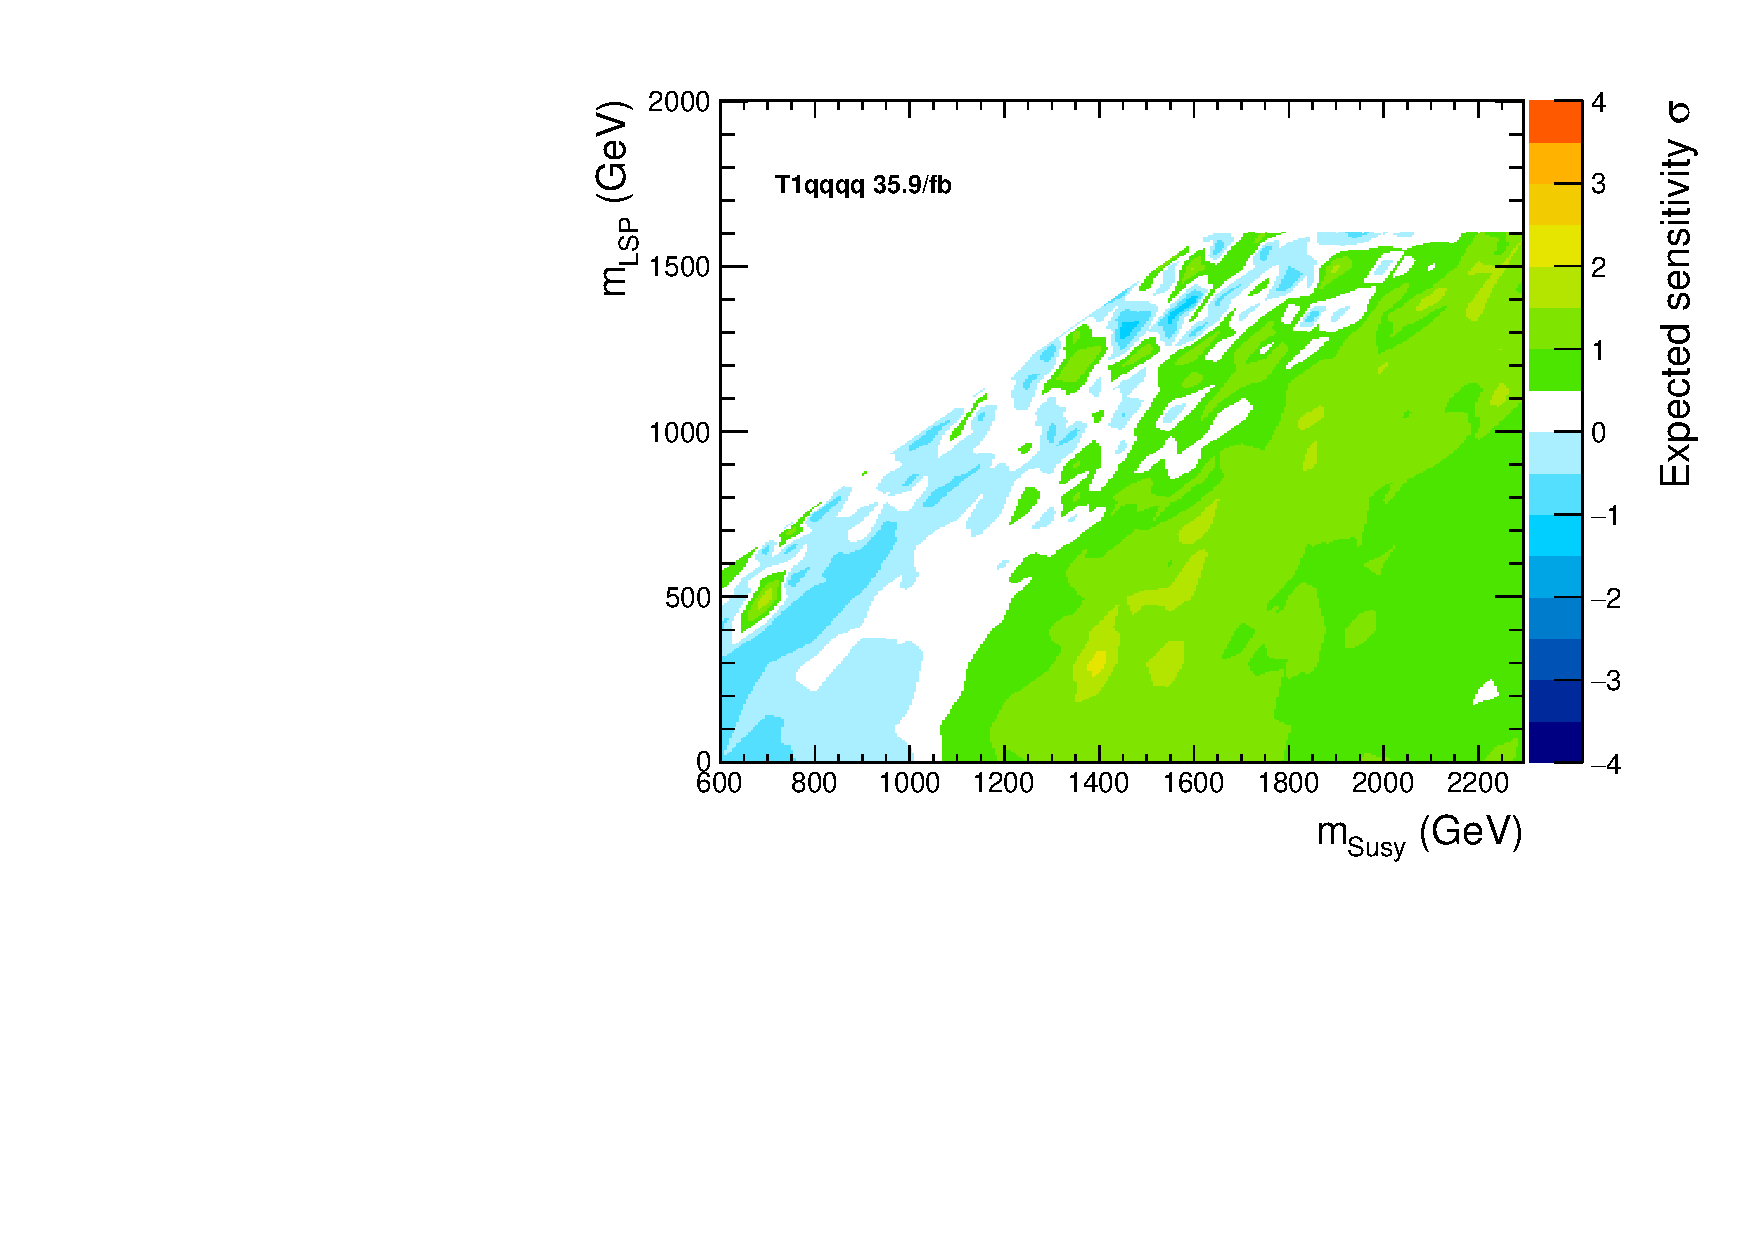
\includegraphics[width=0.45\linewidth]{figures/LLPResults/T1qqqqLL_ctau-1_signif}
        %    \label{fig:T1qqqqLL_signif_ctau-100000}
        %} ~~
        \caption{Top: the 95\% C.L. observed upper limit on the cross section
            (histogram), with the expected (solid black line) observed
            (solid red line) exclusion contours. Left: signal acceptance
            including all jet categories. Right: graph showing the most 
            sensitive event topologies for each mass point.
            %Bottom: local observed significance scan.
        }
        \label{fig:T1qqqqLL:ctau-100000}
    \end{center}
\end{figure}
